\documentclass{article}
\usepackage{graphicx}
\usepackage{authblk}
\usepackage{amsmath}
\usepackage{listings}

\begin{document}


\title{THEORETICAL NEUROSCIENCE II \\ EXERCISE 07 - POLICY LEARNING}
\date{16 June 2013}
\author[1]{Yunus Emre Demiray, Taygun C. Uzuneser, \c{S}eyma Bayrak\thanks{seyma.bayrak@st.ovgu.de}}
\affil[1]{\footnotesize  Otto von Guericke University of Magdeburg}
\maketitle

\newpage

\section{Introduction}

This exercise aims to introduce the policy learning with the example of bees which forage among flowers in search for nectar. It is supposed that bees forage under controlled conditions among flowers, after many visits to different colored flowers, the bees learn the reward characteristics. With this reward learning, they tend to visit the more rewarding color. Later on, the reward characteristics of flowers are changed, and we anaylze the new preference of the bees, if they change their preferences. 

The probability of visiting the red flower is denoted by $P_r$, and that of the blue flower is denote by $P_b$. With the introduced action values $m_r$ and $m_b$, the probabilities are defined as the following:
\begin{equation}
 P_r=\frac{1}{1+exp(\beta ({\bar m}-m_r))} \;\;\;\;\;\;\;\;\;\; P_b=\frac{1}{1+exp(\beta ({\bar m}-m_b))}
\end{equation}
\begin{equation}
  P_r+P_b=1\;\;\;\;\;\;\;\;\;\; {\bar m}=\frac{1}{2}(m_r+m_b)
\end{equation}
where the constant $\beta$ determines the variability of the bee's choice. The action values will $m_r$ and $m_b$ evolve with the learned reinforcement, they will be analyzed in more detail in later sections. 

\subsection{Changing Rewards}
The rewards for the red and blue flowers are assigned to canstant values. However, the exercise asks to create two different phases; first phase and second phase are assumed to change their reward values. 

The average and variance values to the reward values in the first phase:
\begin{equation*}
 \langle r_r \rangle= 3, \;\;\;\;\; \langle r_r ^2 \rangle -\langle r_r \rangle ^2 =1
\end{equation*}
\begin{equation*}
 \langle r_b \rangle= 1, \;\;\;\;\; \langle r_b ^2 \rangle -\langle r_b \rangle ^2 =1
\end{equation*}

The average and variance values to the reward values in the second phase:
 \begin{equation*}
 \langle r_r \rangle= 1, \;\;\;\;\; \langle r_r ^2 \rangle -\langle r_r \rangle ^2 =1
\end{equation*}
\begin{equation*}
 \langle r_b \rangle= 3, \;\;\;\;\; \langle r_b ^2 \rangle -\langle r_b \rangle ^2 =1
\end{equation*}

\section{Indirect Actor}
We begin with $m_r=m_b=0$ to simulate the bee's visit with probabilities $P_r$ and $P_b$. The action values are adjusted with indirect actor (Rescola-Wagner) rule:

\textbf{Chose Red:}
\begin{equation*}
 m_r\rightarrow m_r +\epsilon \delta_r \;\;\;\;\;\;\; m_b\rightarrow m_b \;\;\;\;\;\;\; \delta_r=r_r-m_r
\end{equation*}

\textbf{Chose Blue:}
\begin{equation*}
 m_b\rightarrow m_b +\epsilon \delta_b \;\;\;\;\;\;\; m_r\rightarrow m_r \;\;\;\;\;\;\; \delta_b=r_b-m_b
\end{equation*}

The cumulative total rewards $R_r$ and $R_b$ collected from the red and blue flowers are given as the following:

\begin{equation*}
 R_r=\sum_{i=j} ^{N_r} r_r(j) \;\;\;\;\;\;\; R_b=\sum_{i=1} ^{N_b} r_b(i) \;\;\;\;\;\;\; N_r+N_b=N
\end{equation*}
where $r_r(j)$ and $r_b(i)$ are the rewards collected on the $j$th visit to the red flower and $i$th visit to the blue flower, and where $N_r$, $N_b$ and $N$ are the number of visits to red, blue or either kind of flowers.  

\subsection{Programming Assignment for Indirect Actor}

\begin{itemize}
 \item \textbf{ $\beta=5$, $\epsilon=0.1$}
\end{itemize}

\begin{center}
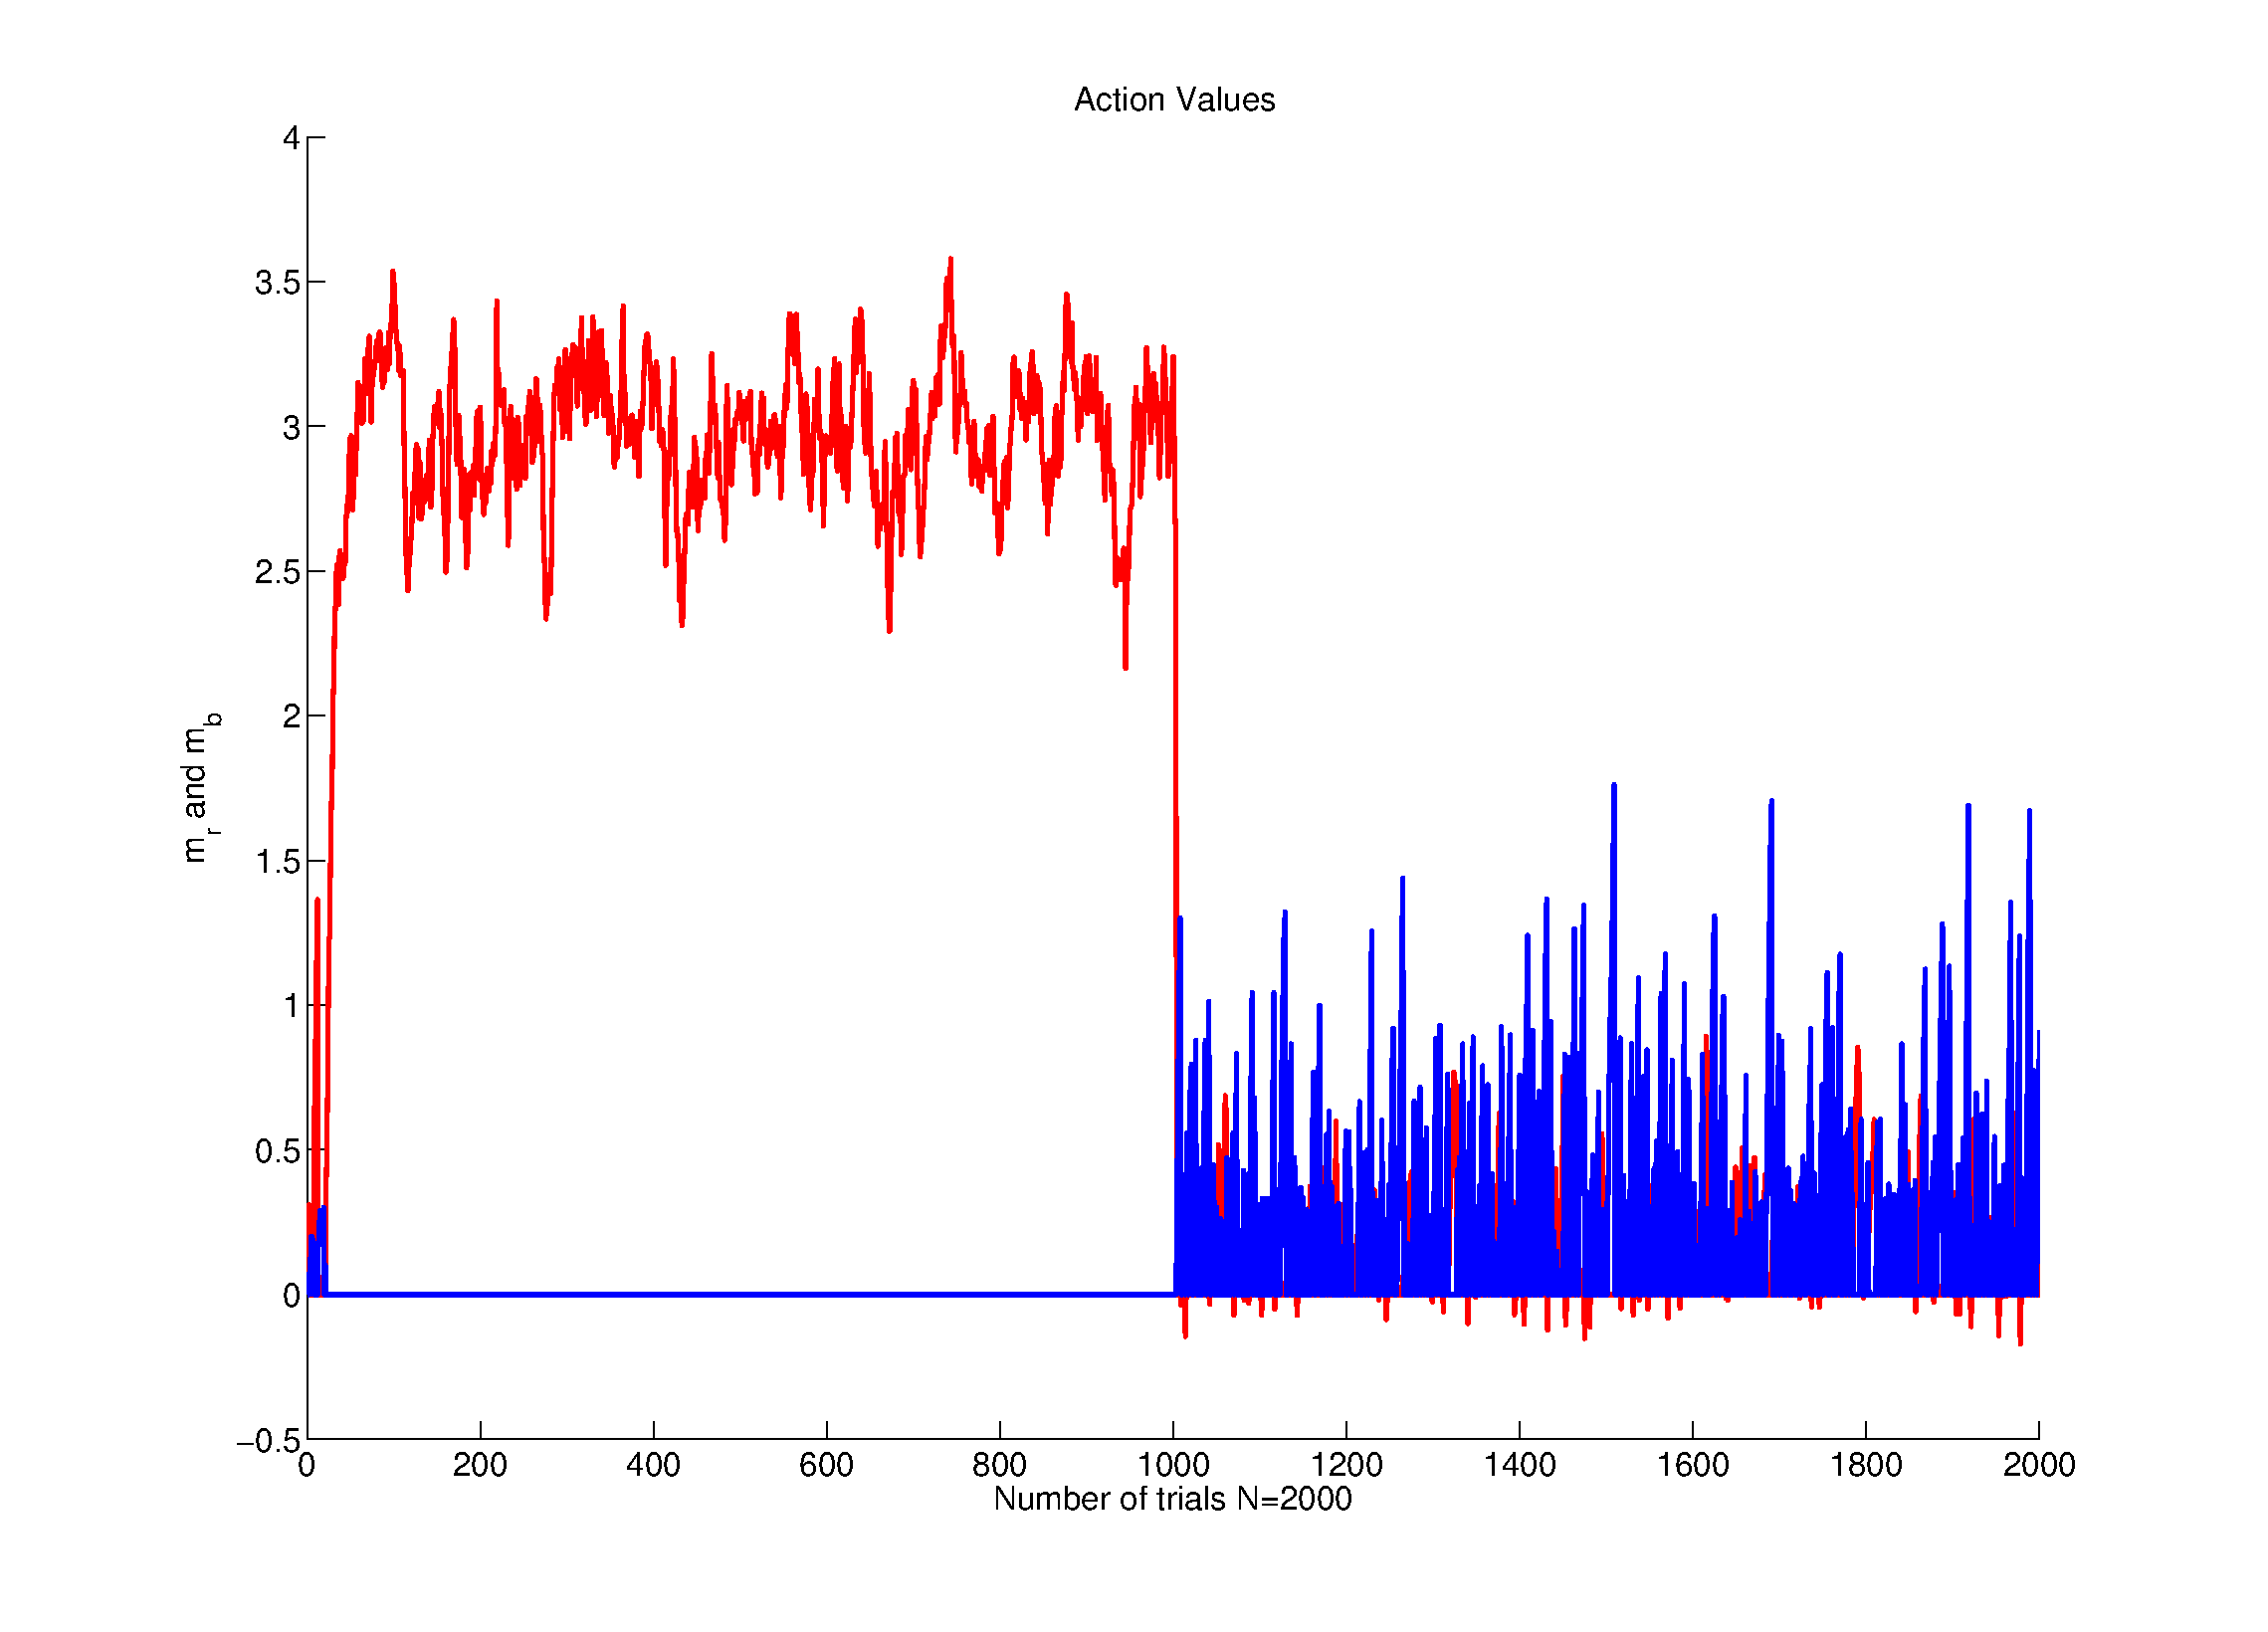
\includegraphics[width=\textwidth]{action1.eps}
% tau4_M1.eps: 0x0 pixel, 300dpi, 0.00x0.00 cm, bb= -304   -42   918   834
\begin{footnotesize}
 Figure 1, $\beta=5$, $\epsilon=0.1$
\end{footnotesize}
\end{center}

\begin{center}
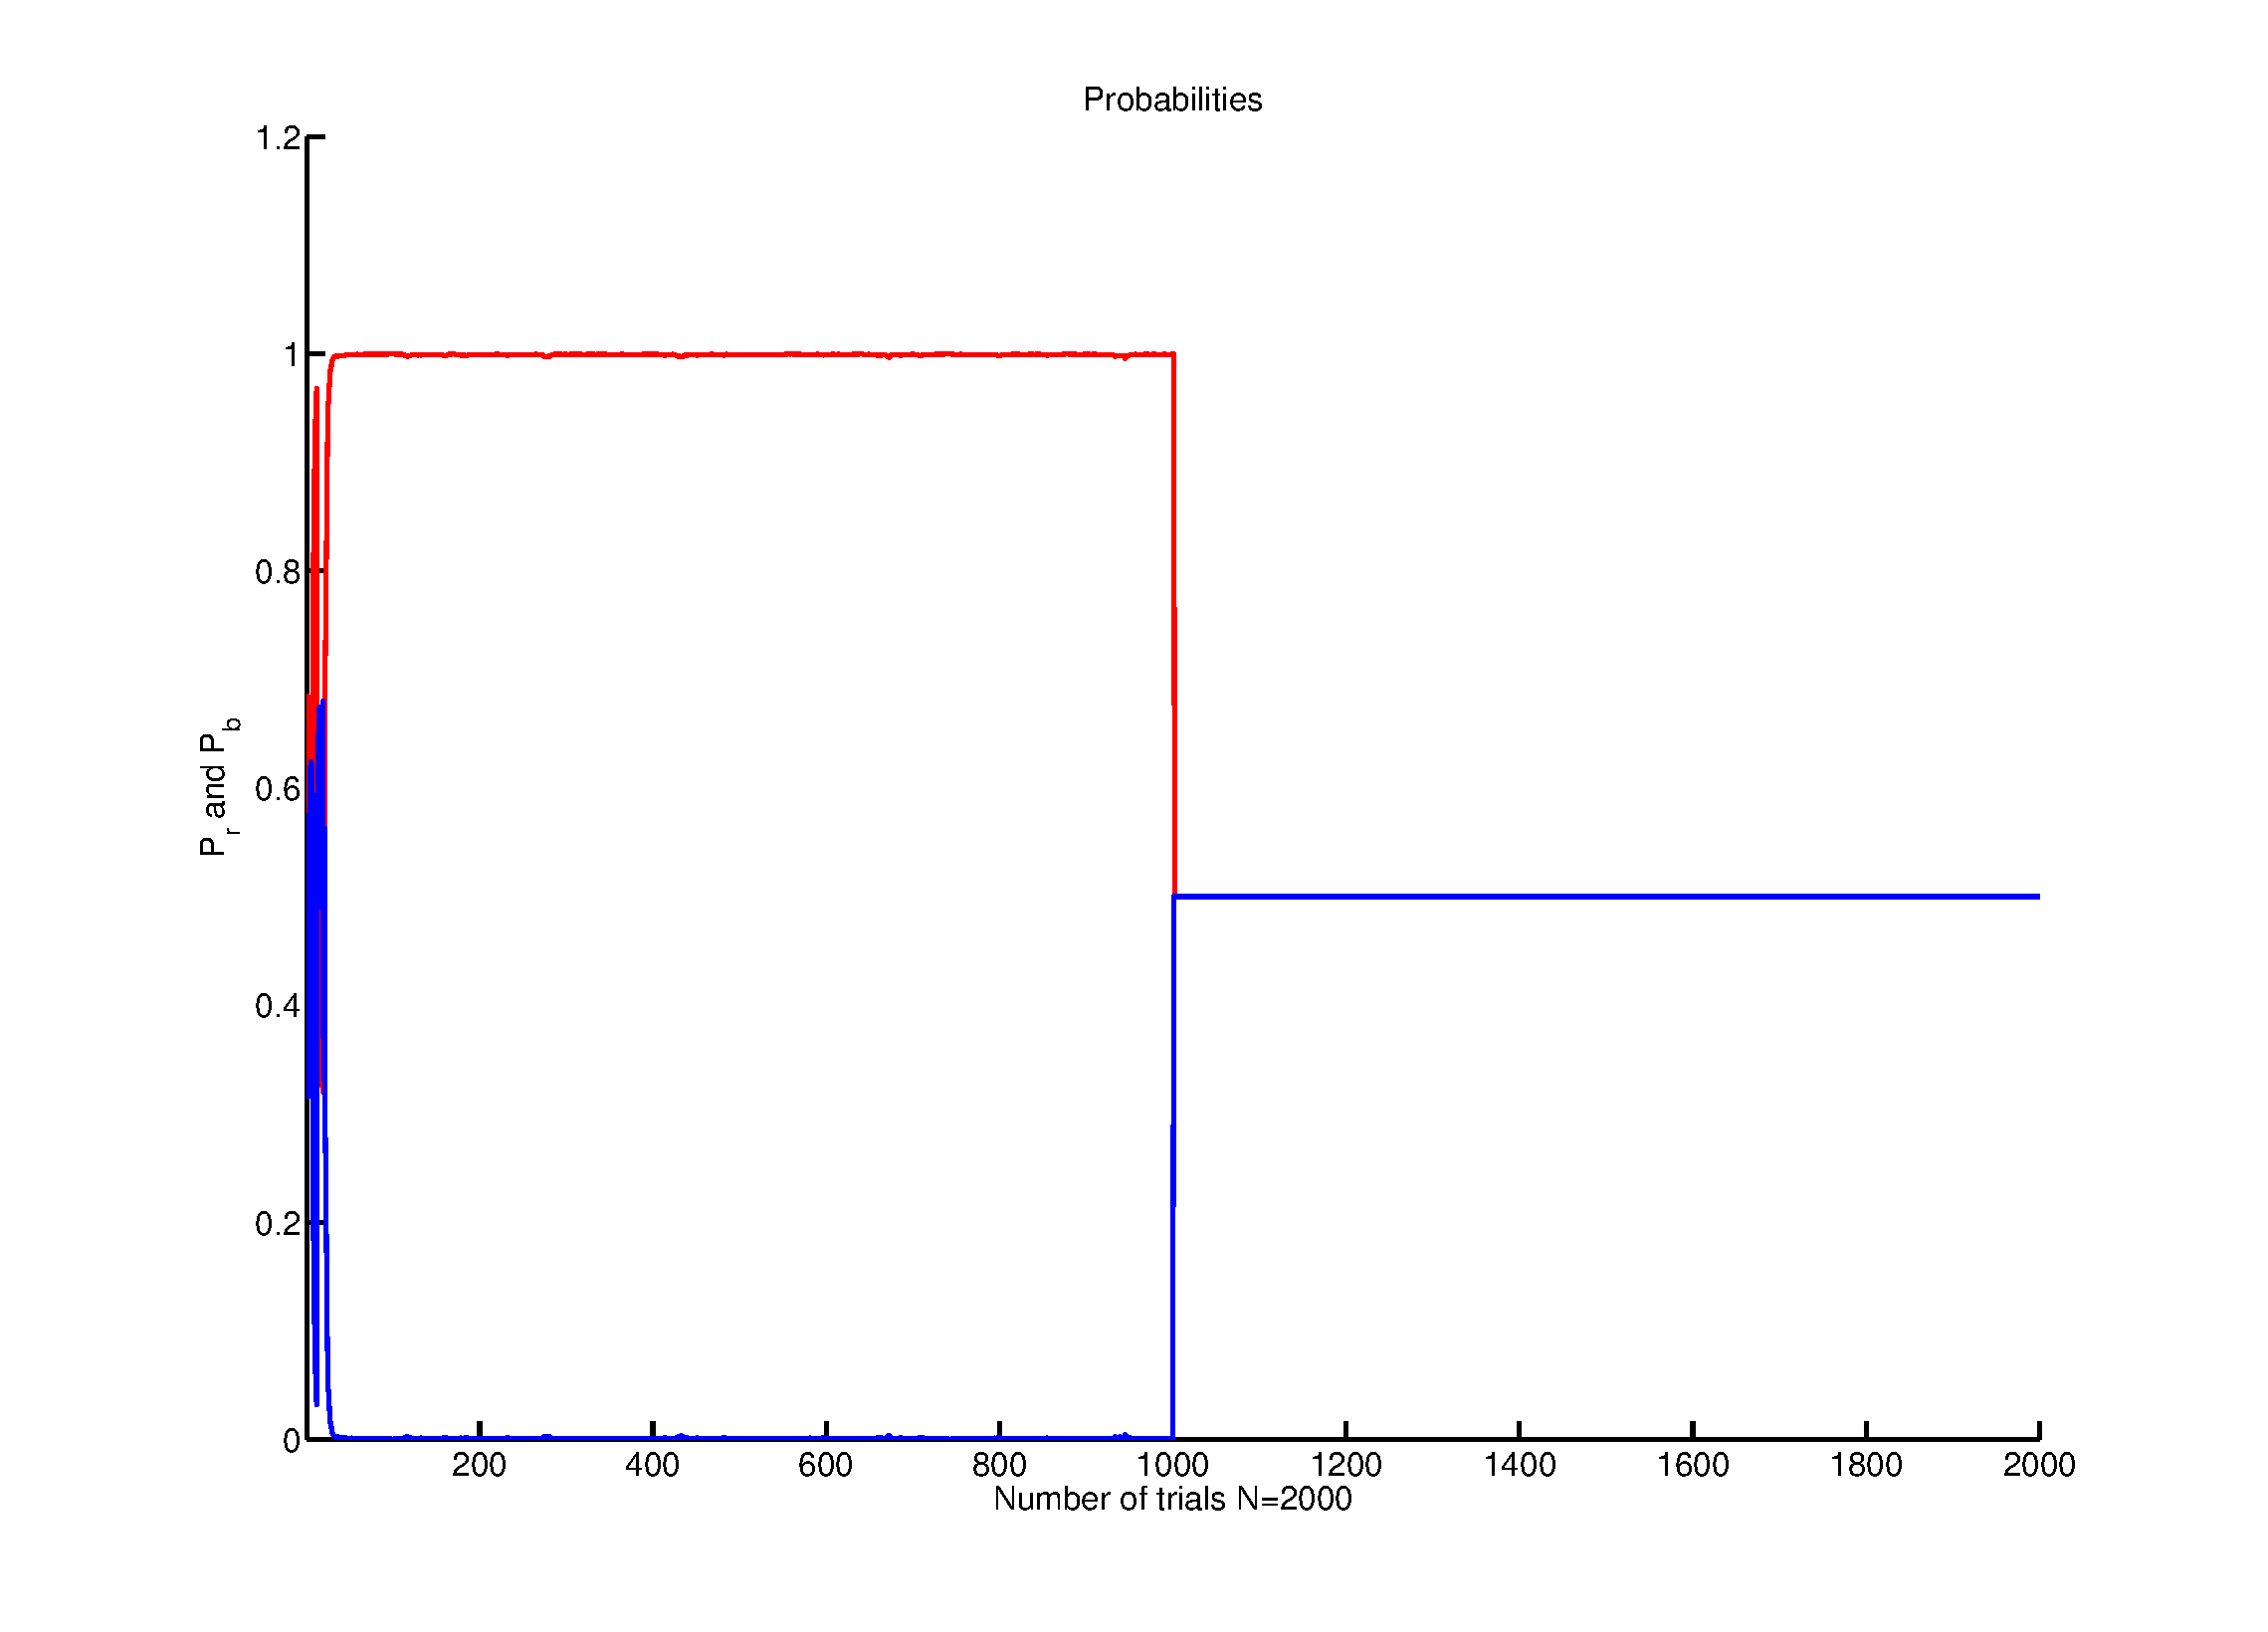
\includegraphics[width=\textwidth]{prob1.eps}
% tau4_M1.eps: 0x0 pixel, 300dpi, 0.00x0.00 cm, bb= -304   -42   918   834
\begin{footnotesize}
 Figure 2, $\beta=5$, $\epsilon=0.1$
\end{footnotesize}
\end{center}

\begin{center}
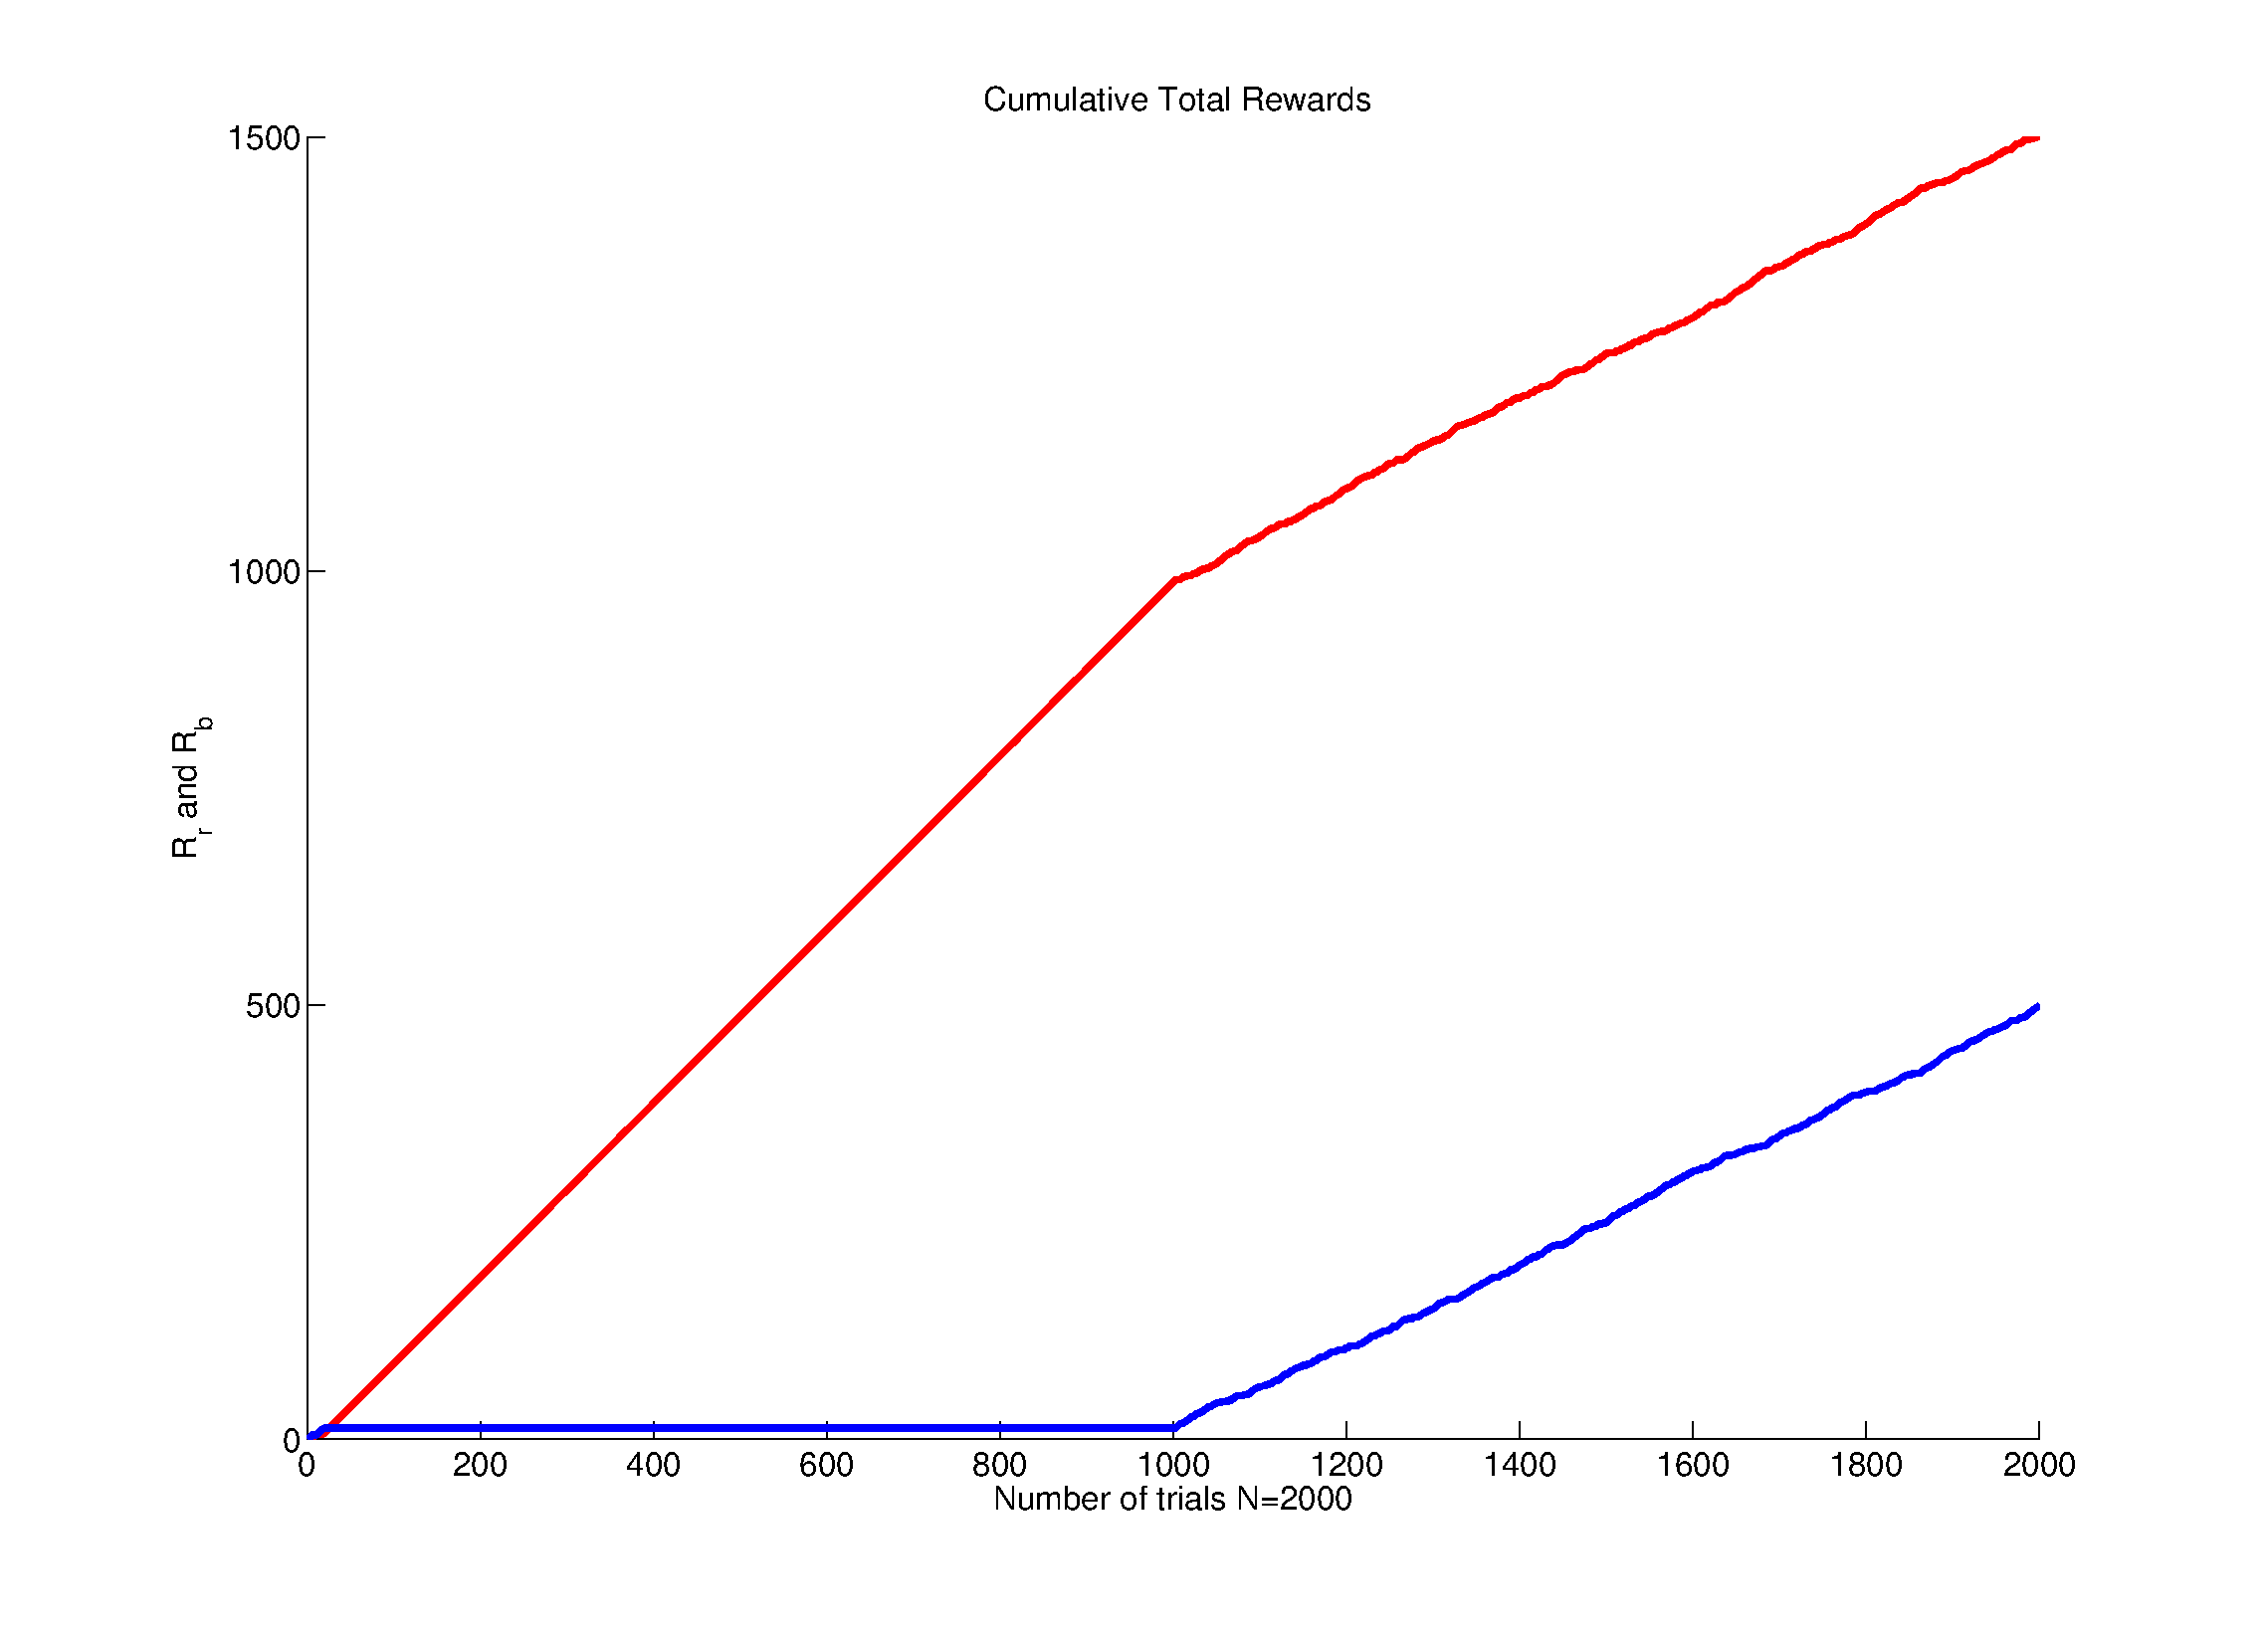
\includegraphics[width=\textwidth]{rew1.eps}
% tau4_M1.eps: 0x0 pixel, 300dpi, 0.00x0.00 cm, bb= -304   -42   918   834
\begin{footnotesize}
 Figure 3, $\beta=5$, $\epsilon=0.1$
\end{footnotesize}
\end{center}

\newpage
\begin{itemize}
 \item \textbf{ $\beta=2$, $\epsilon=0.1$}
\end{itemize}

\begin{center}
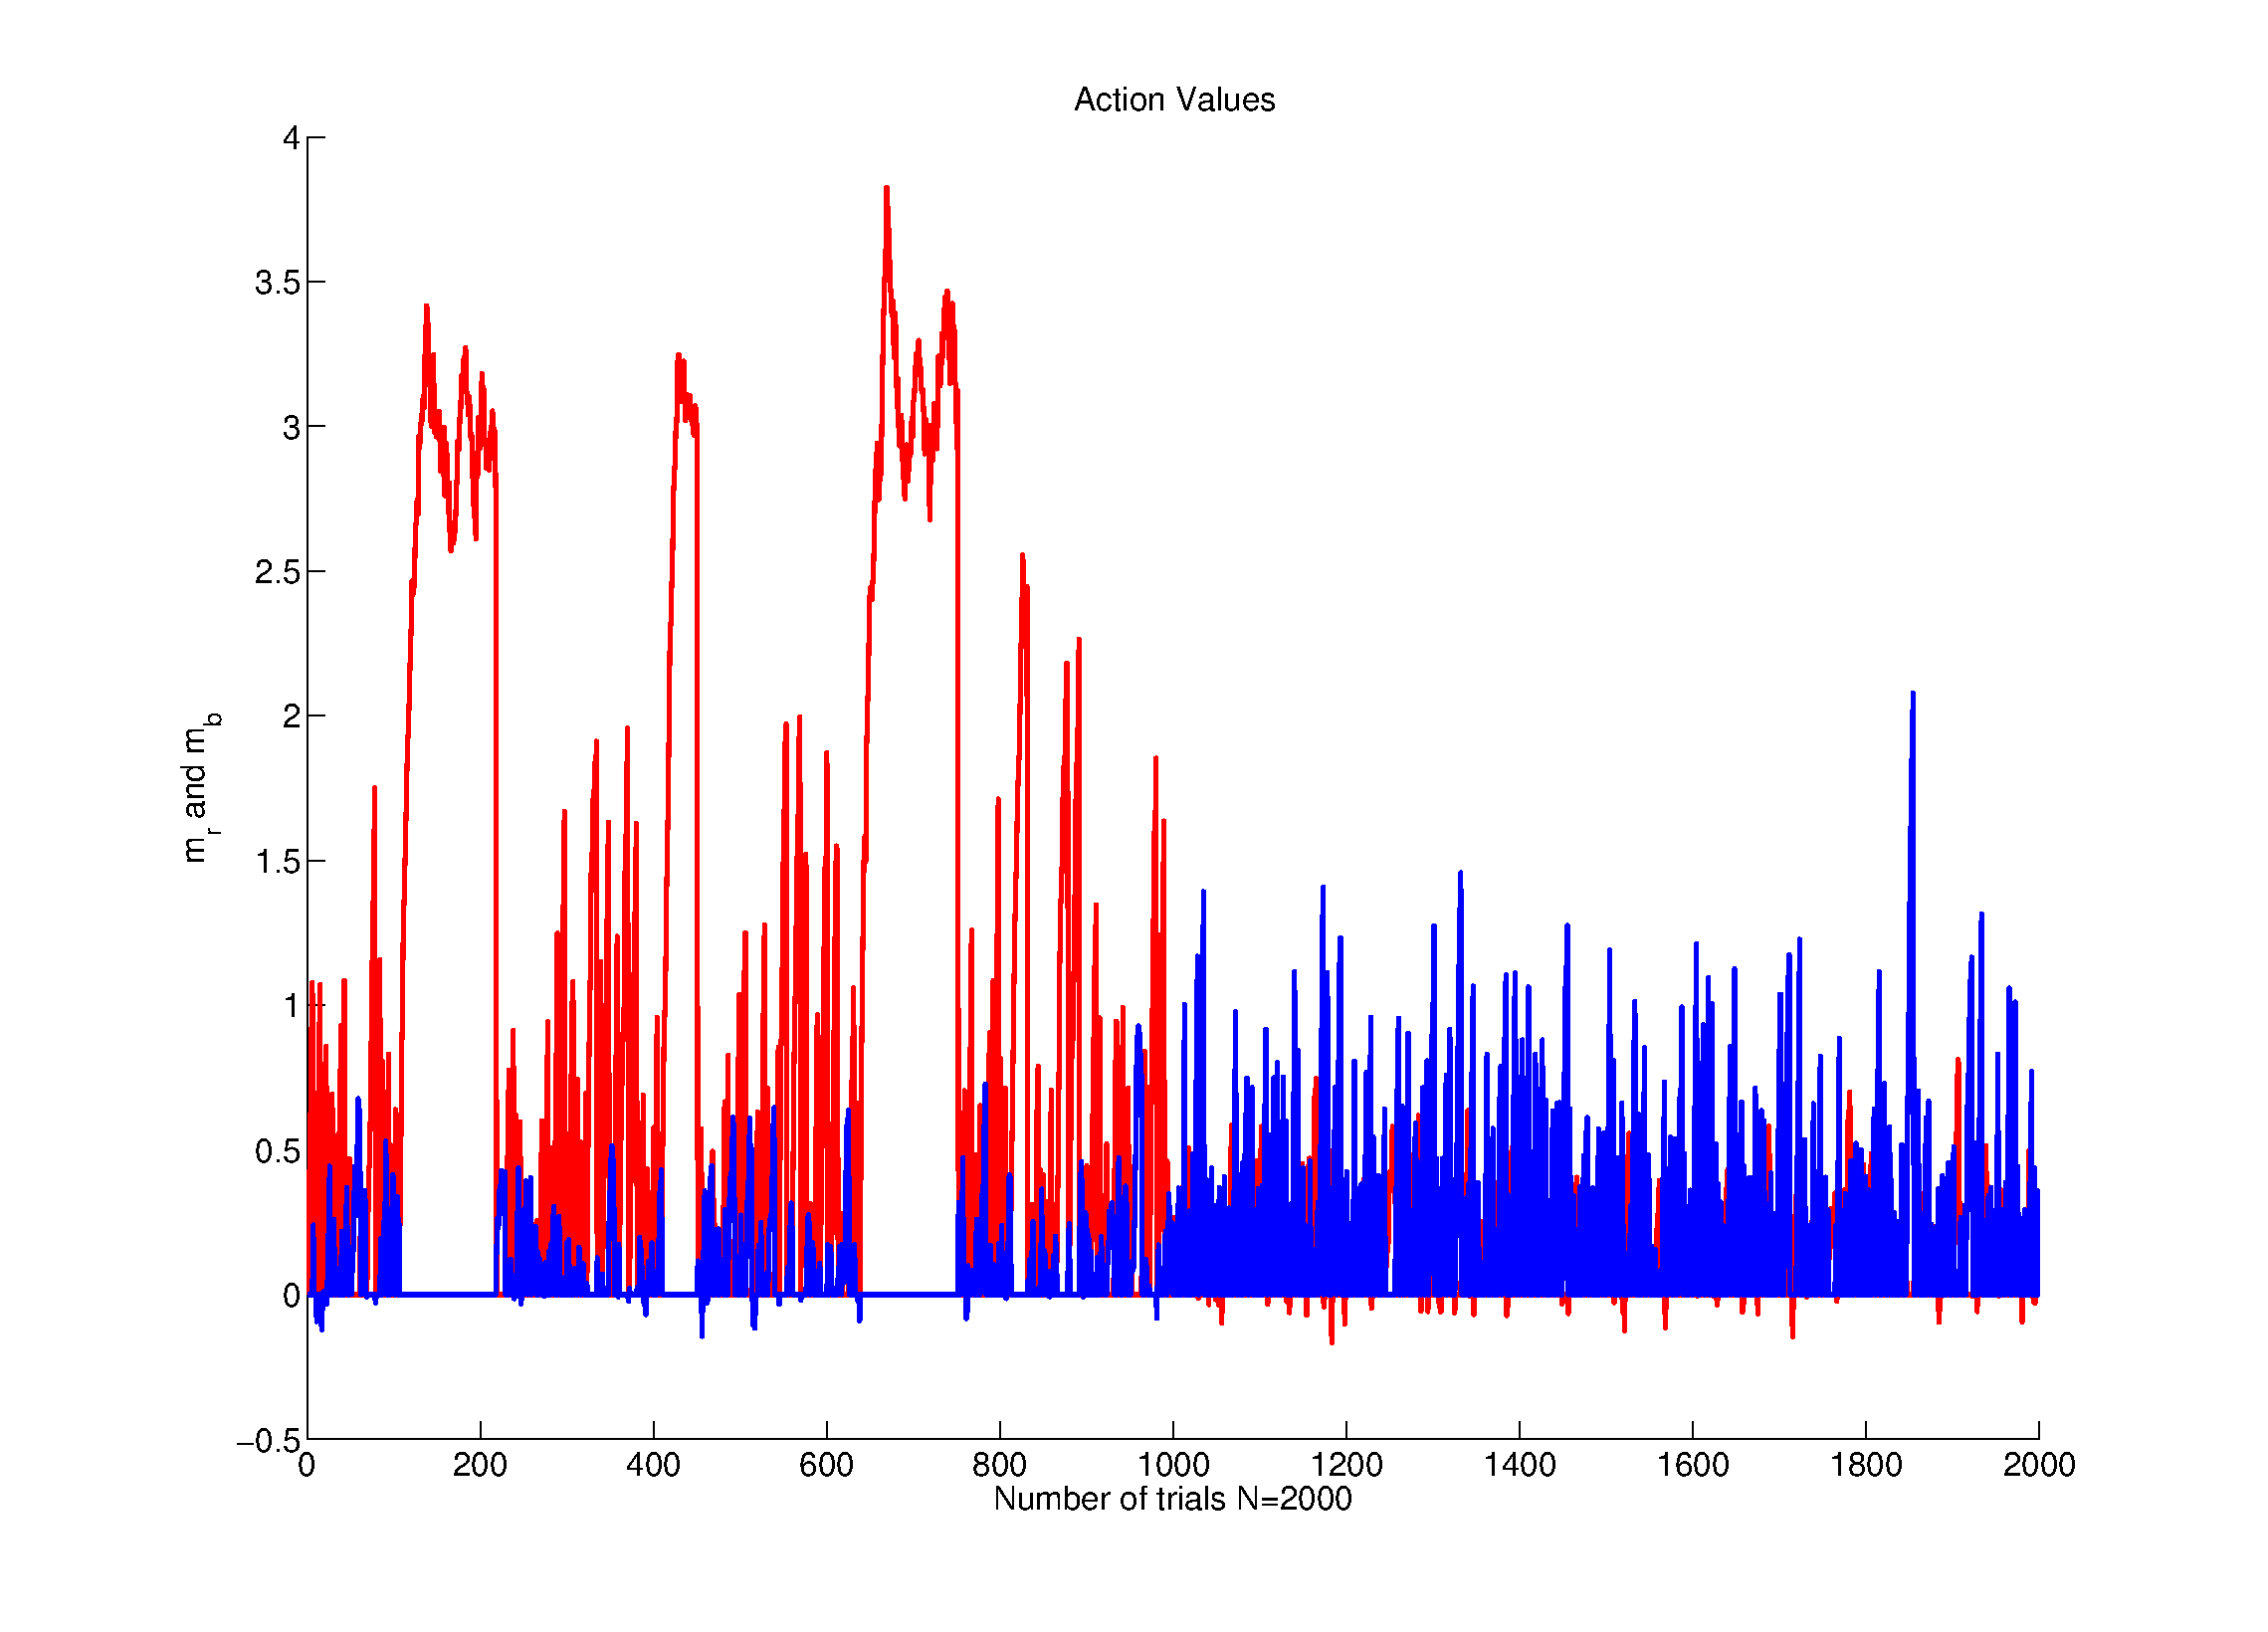
\includegraphics[width=\textwidth]{action2.eps}
% tau4_M1.eps: 0x0 pixel, 300dpi, 0.00x0.00 cm, bb= -304   -42   918   834
\begin{footnotesize}
 Figure 4, $\beta=2$, $\epsilon=0.1$
\end{footnotesize}
\end{center}

\begin{center}
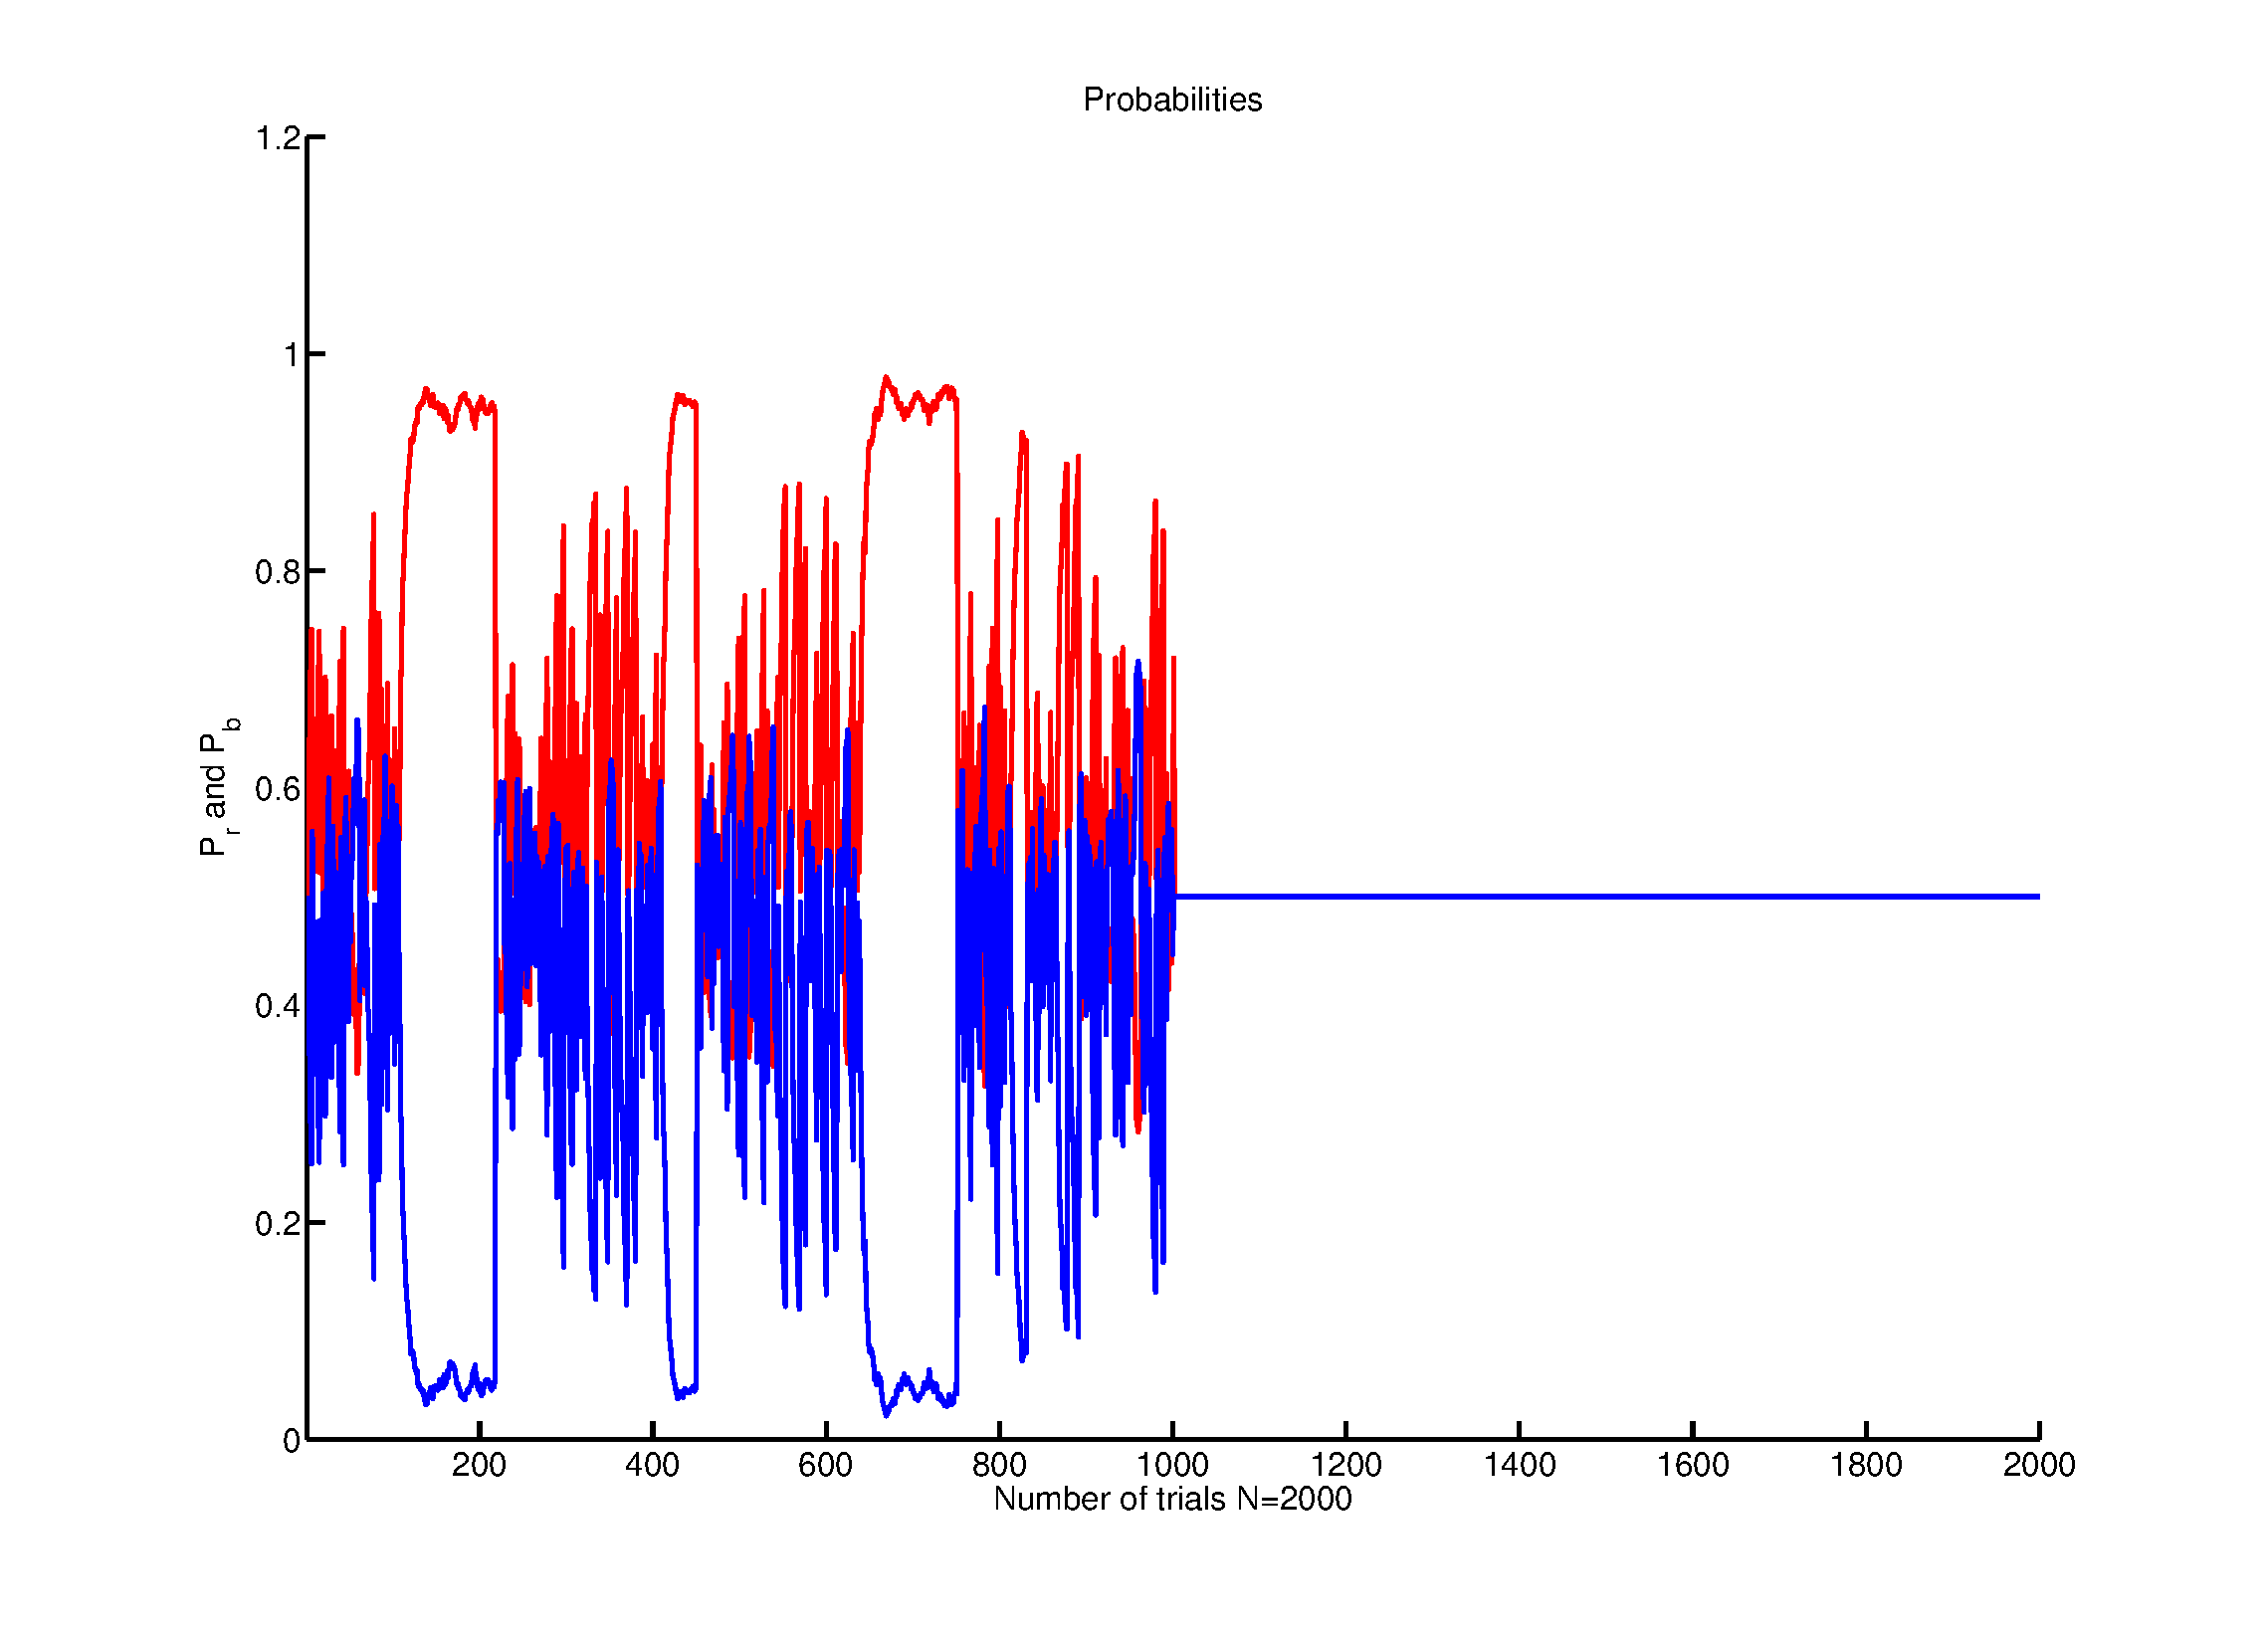
\includegraphics[width=\textwidth]{prob2.eps}
% tau4_M1.eps: 0x0 pixel, 300dpi, 0.00x0.00 cm, bb= -304   -42   918   834
\begin{footnotesize}
 Figure 5, $\beta=2$, $\epsilon=0.1$
\end{footnotesize}
\end{center}

\begin{center}
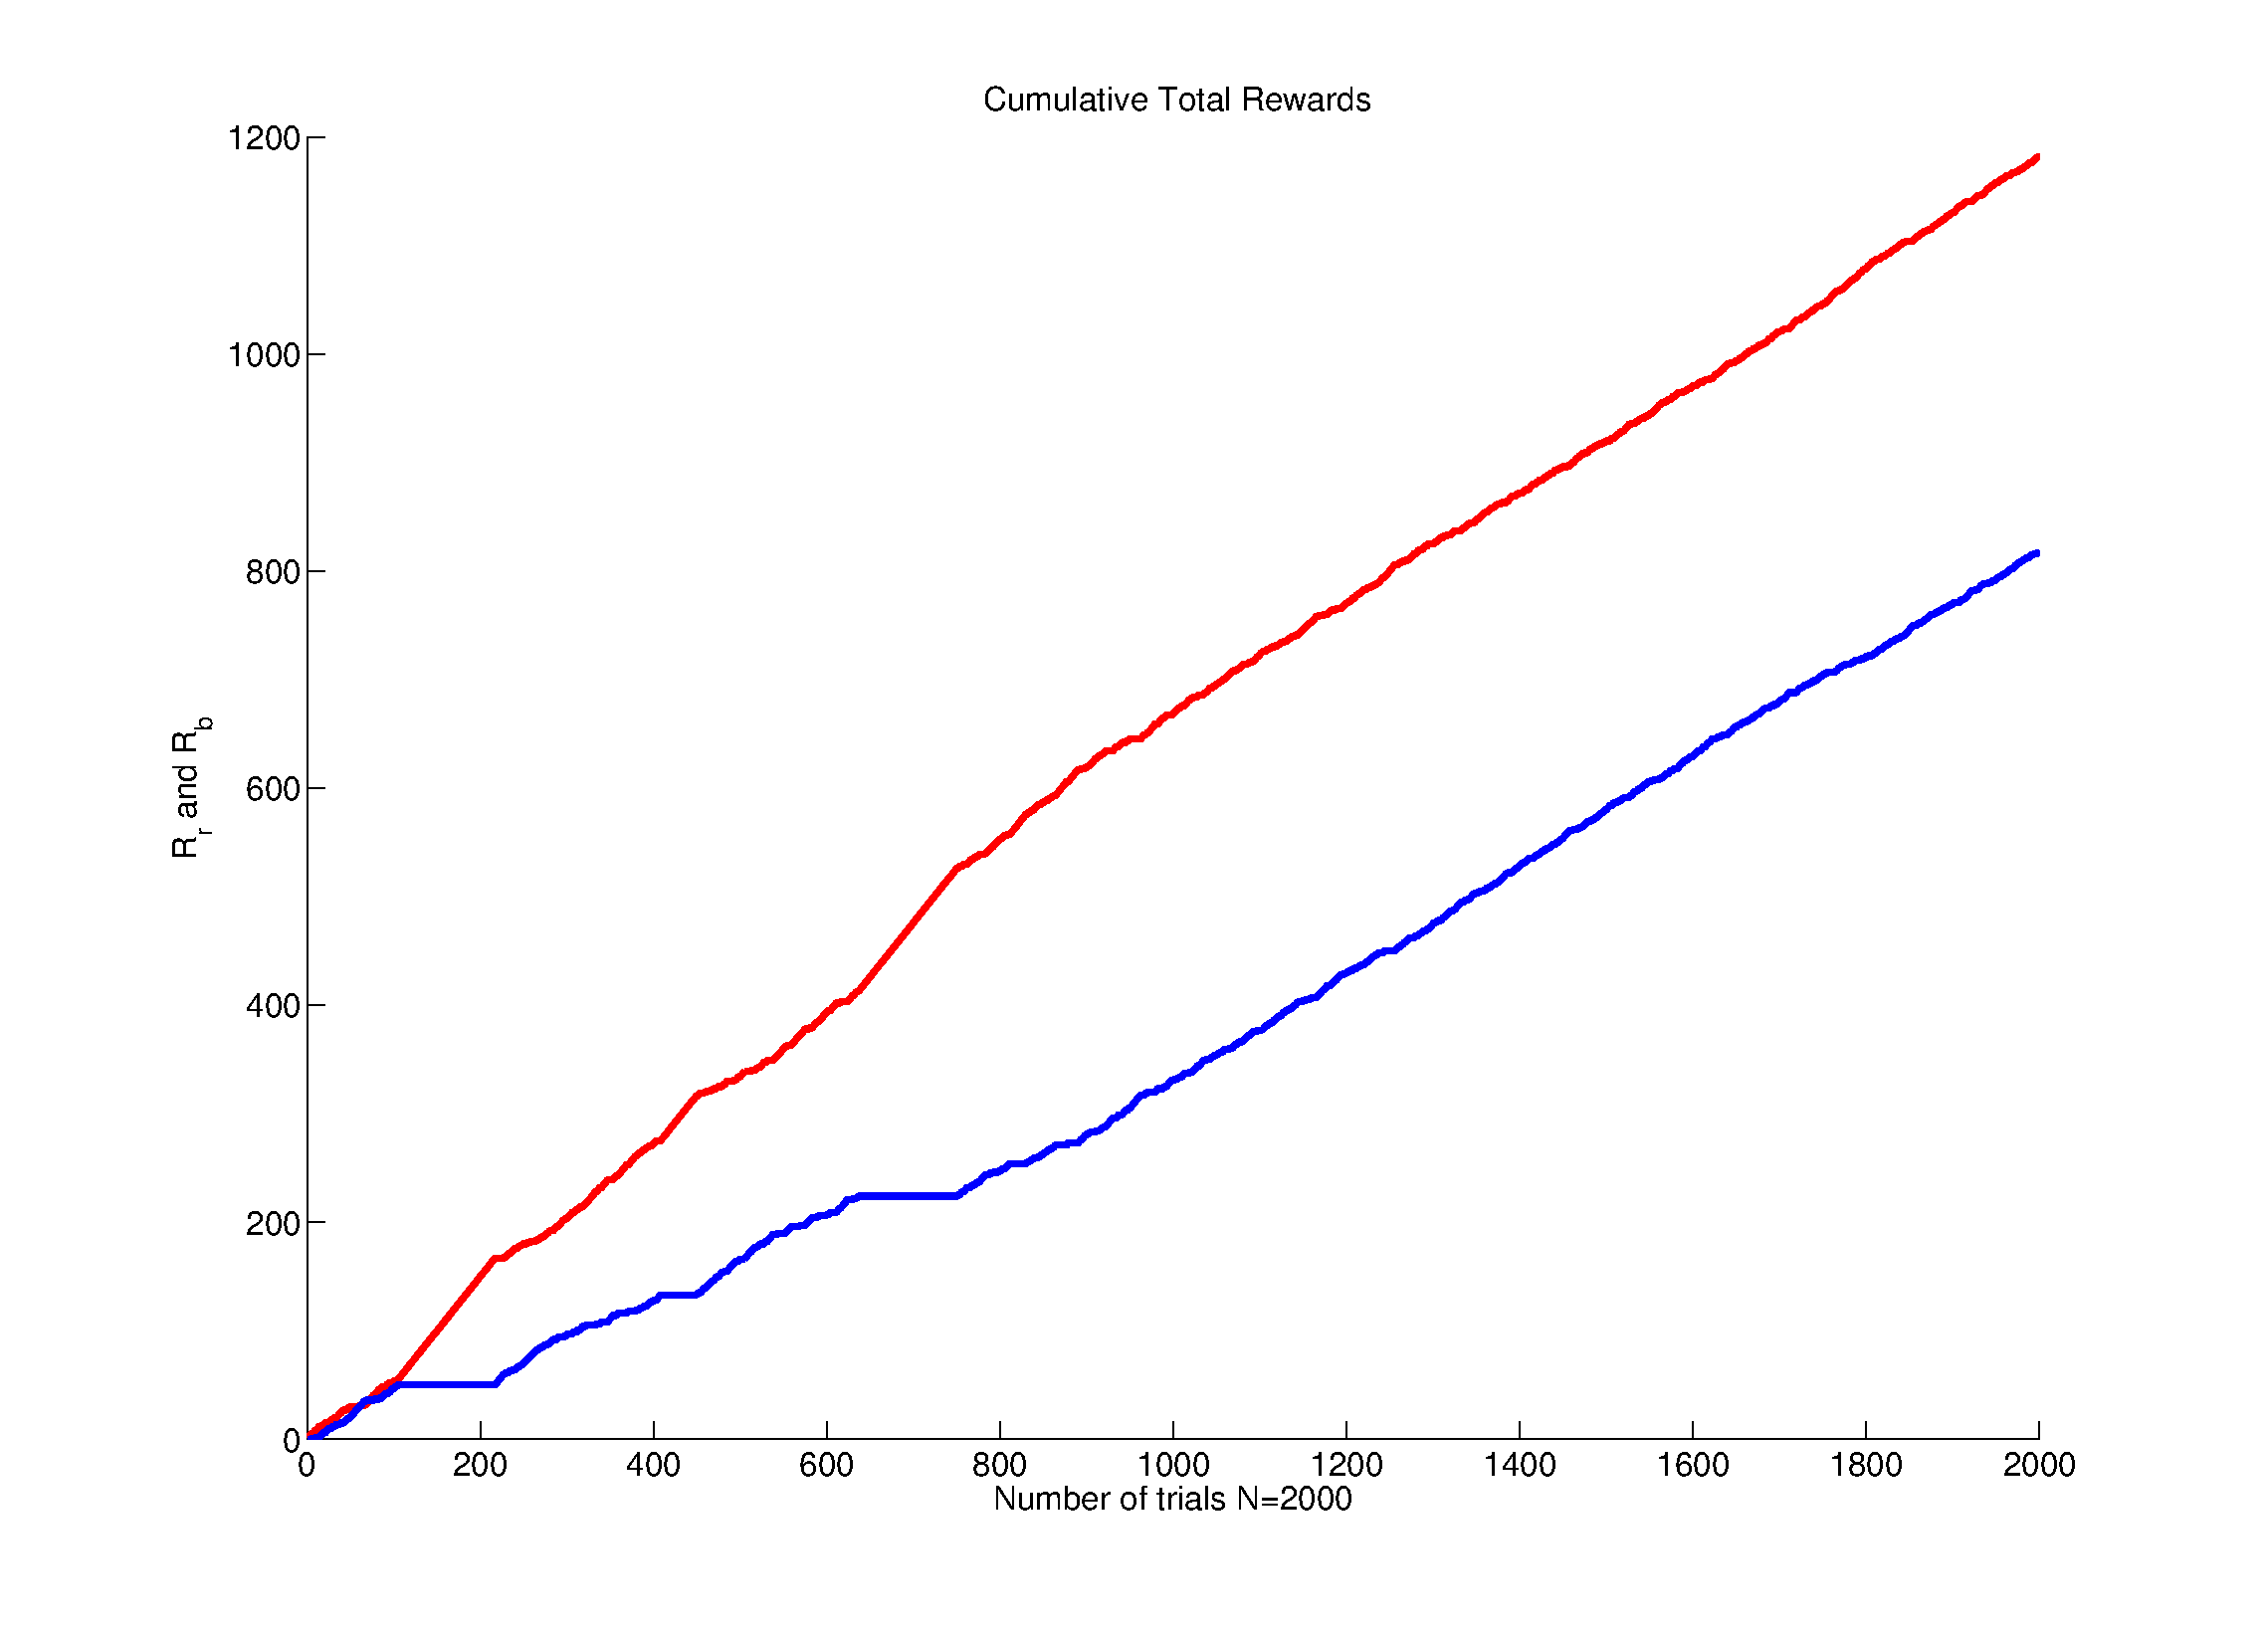
\includegraphics[width=\textwidth]{rew2.eps}
% tau4_M1.eps: 0x0 pixel, 300dpi, 0.00x0.00 cm, bb= -304   -42   918   834
\begin{footnotesize}
 Figure 6, $\beta=2$, $\epsilon=0.1$
\end{footnotesize}
\end{center}

\begin{itemize}
 \item \textbf{ $\beta=20$, $\epsilon=0.1$}
\end{itemize}

\begin{center}
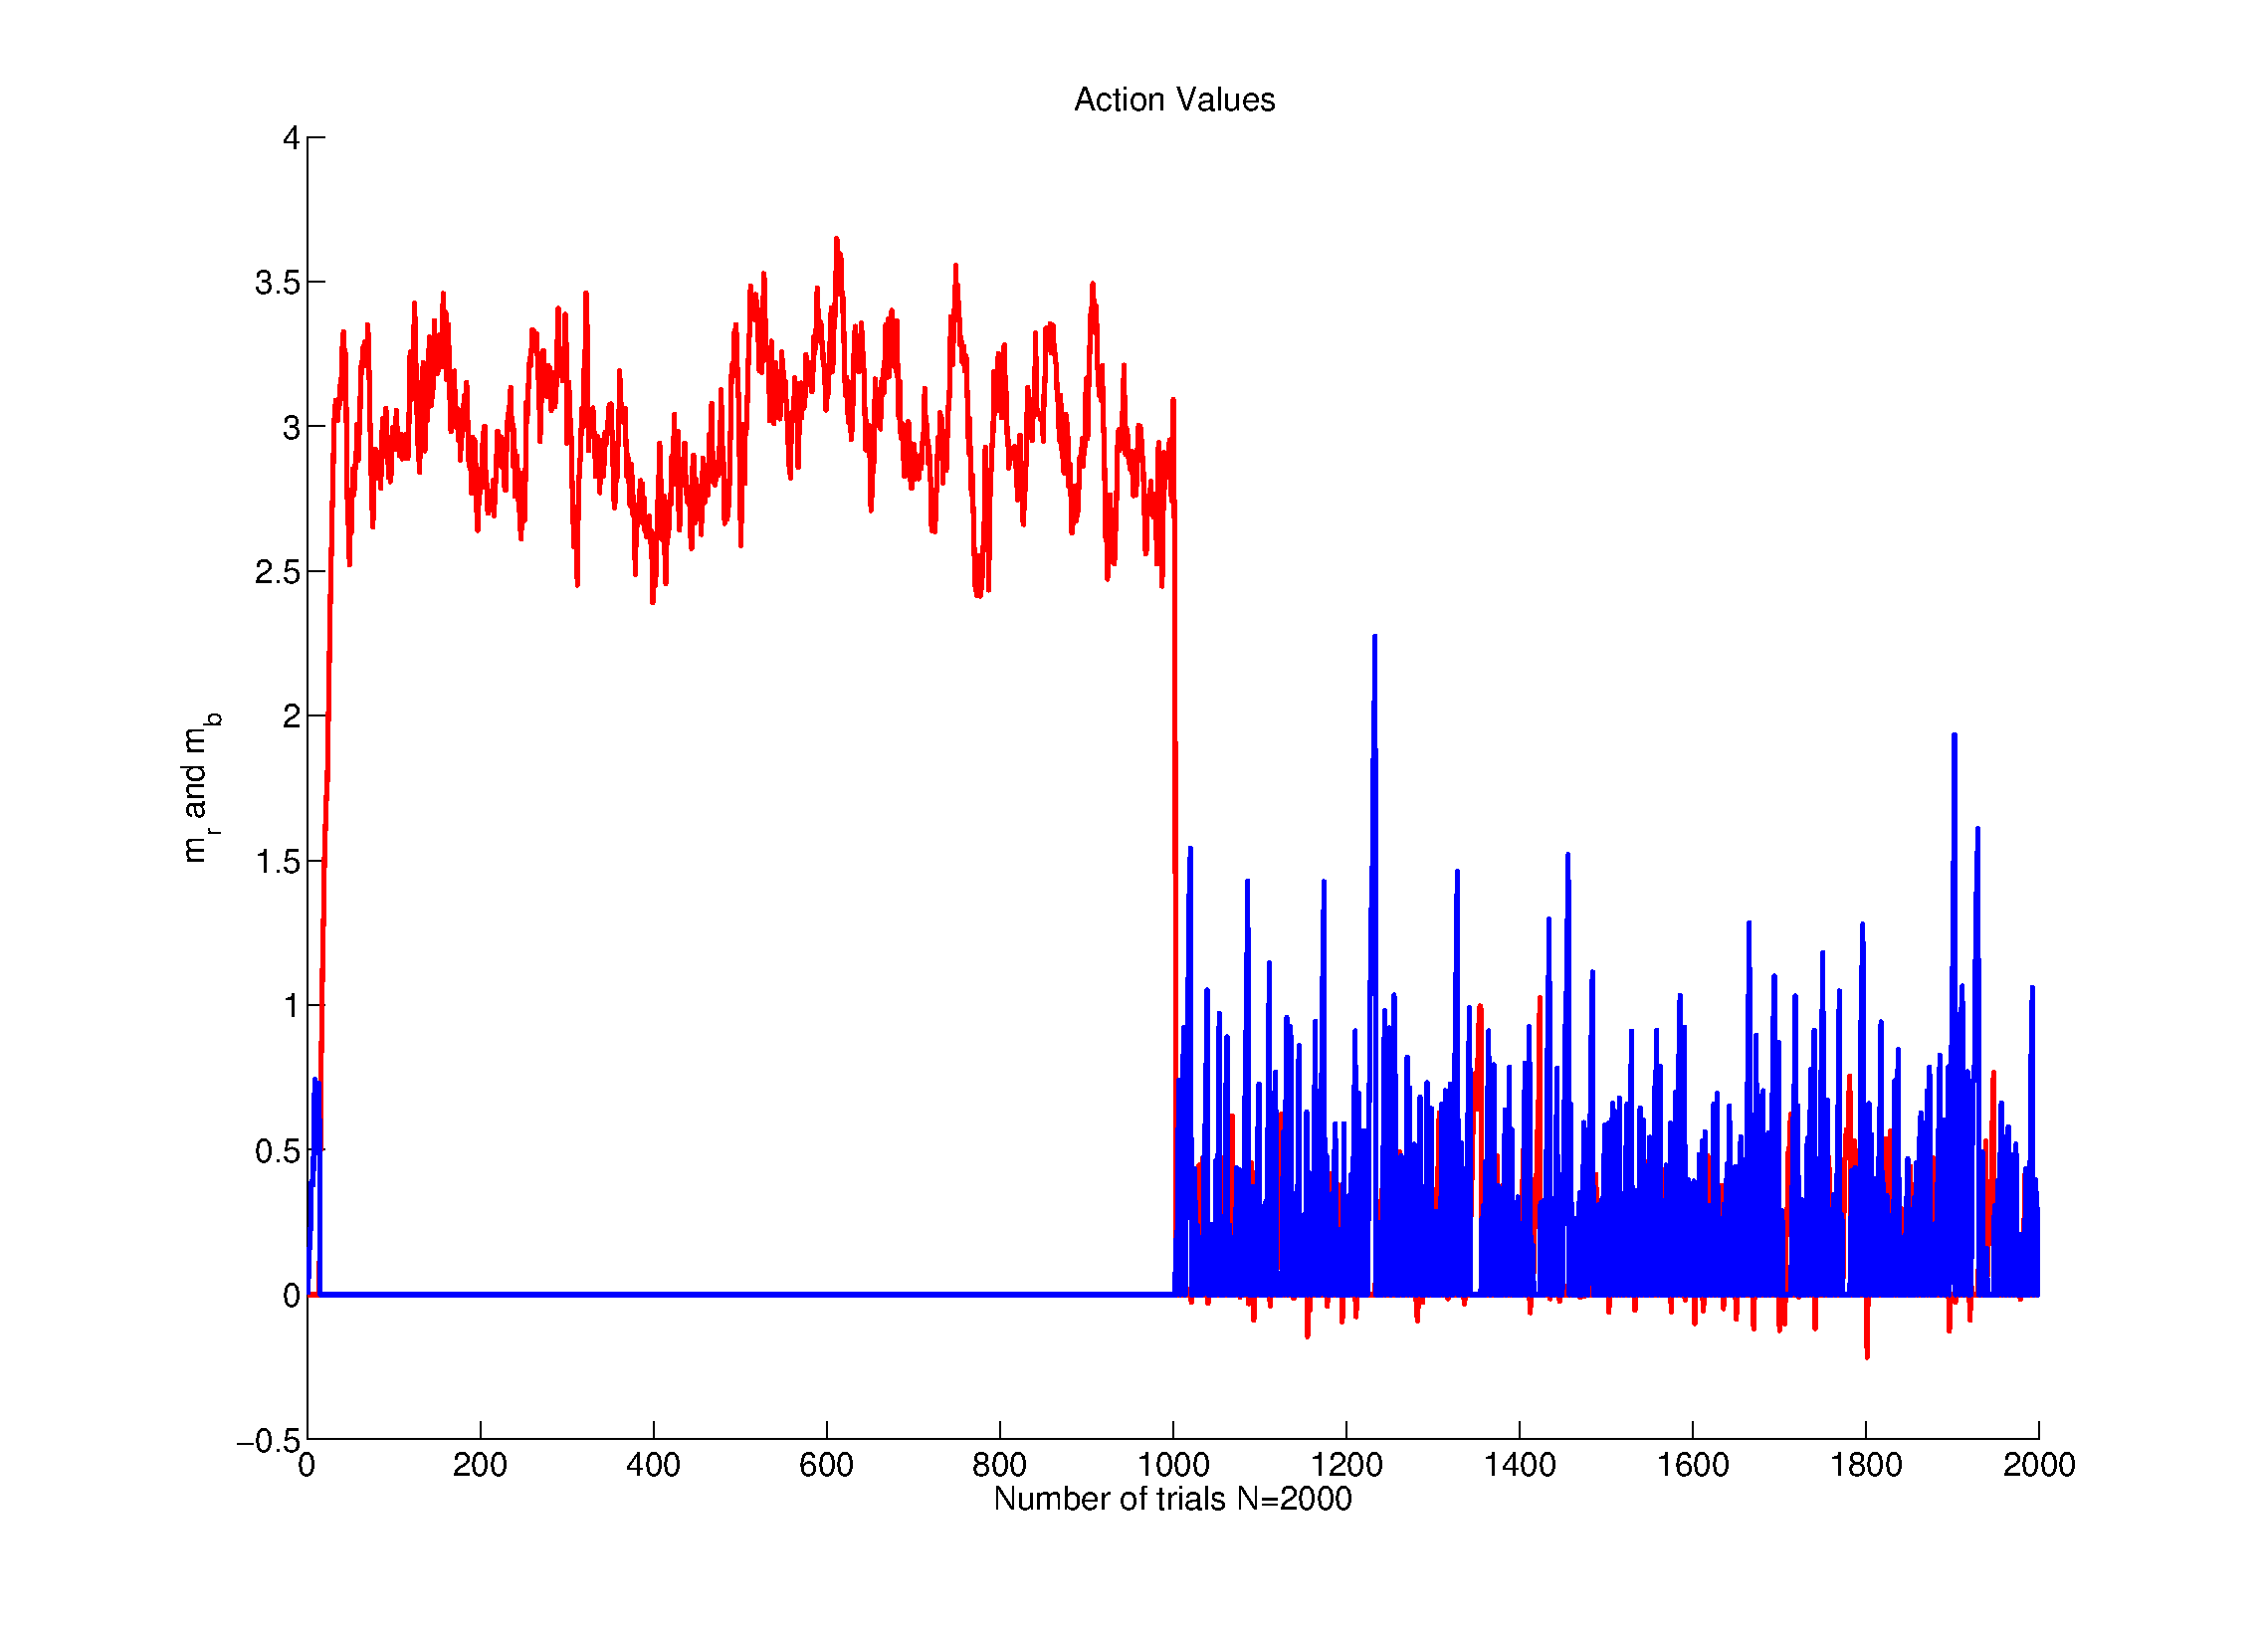
\includegraphics[width=\textwidth]{action3.eps}
% tau4_M1.eps: 0x0 pixel, 300dpi, 0.00x0.00 cm, bb= -304   -42   918   834
\begin{footnotesize}
 Figure 7, $\beta=20$, $\epsilon=0.1$
\end{footnotesize}
\end{center}

\begin{center}
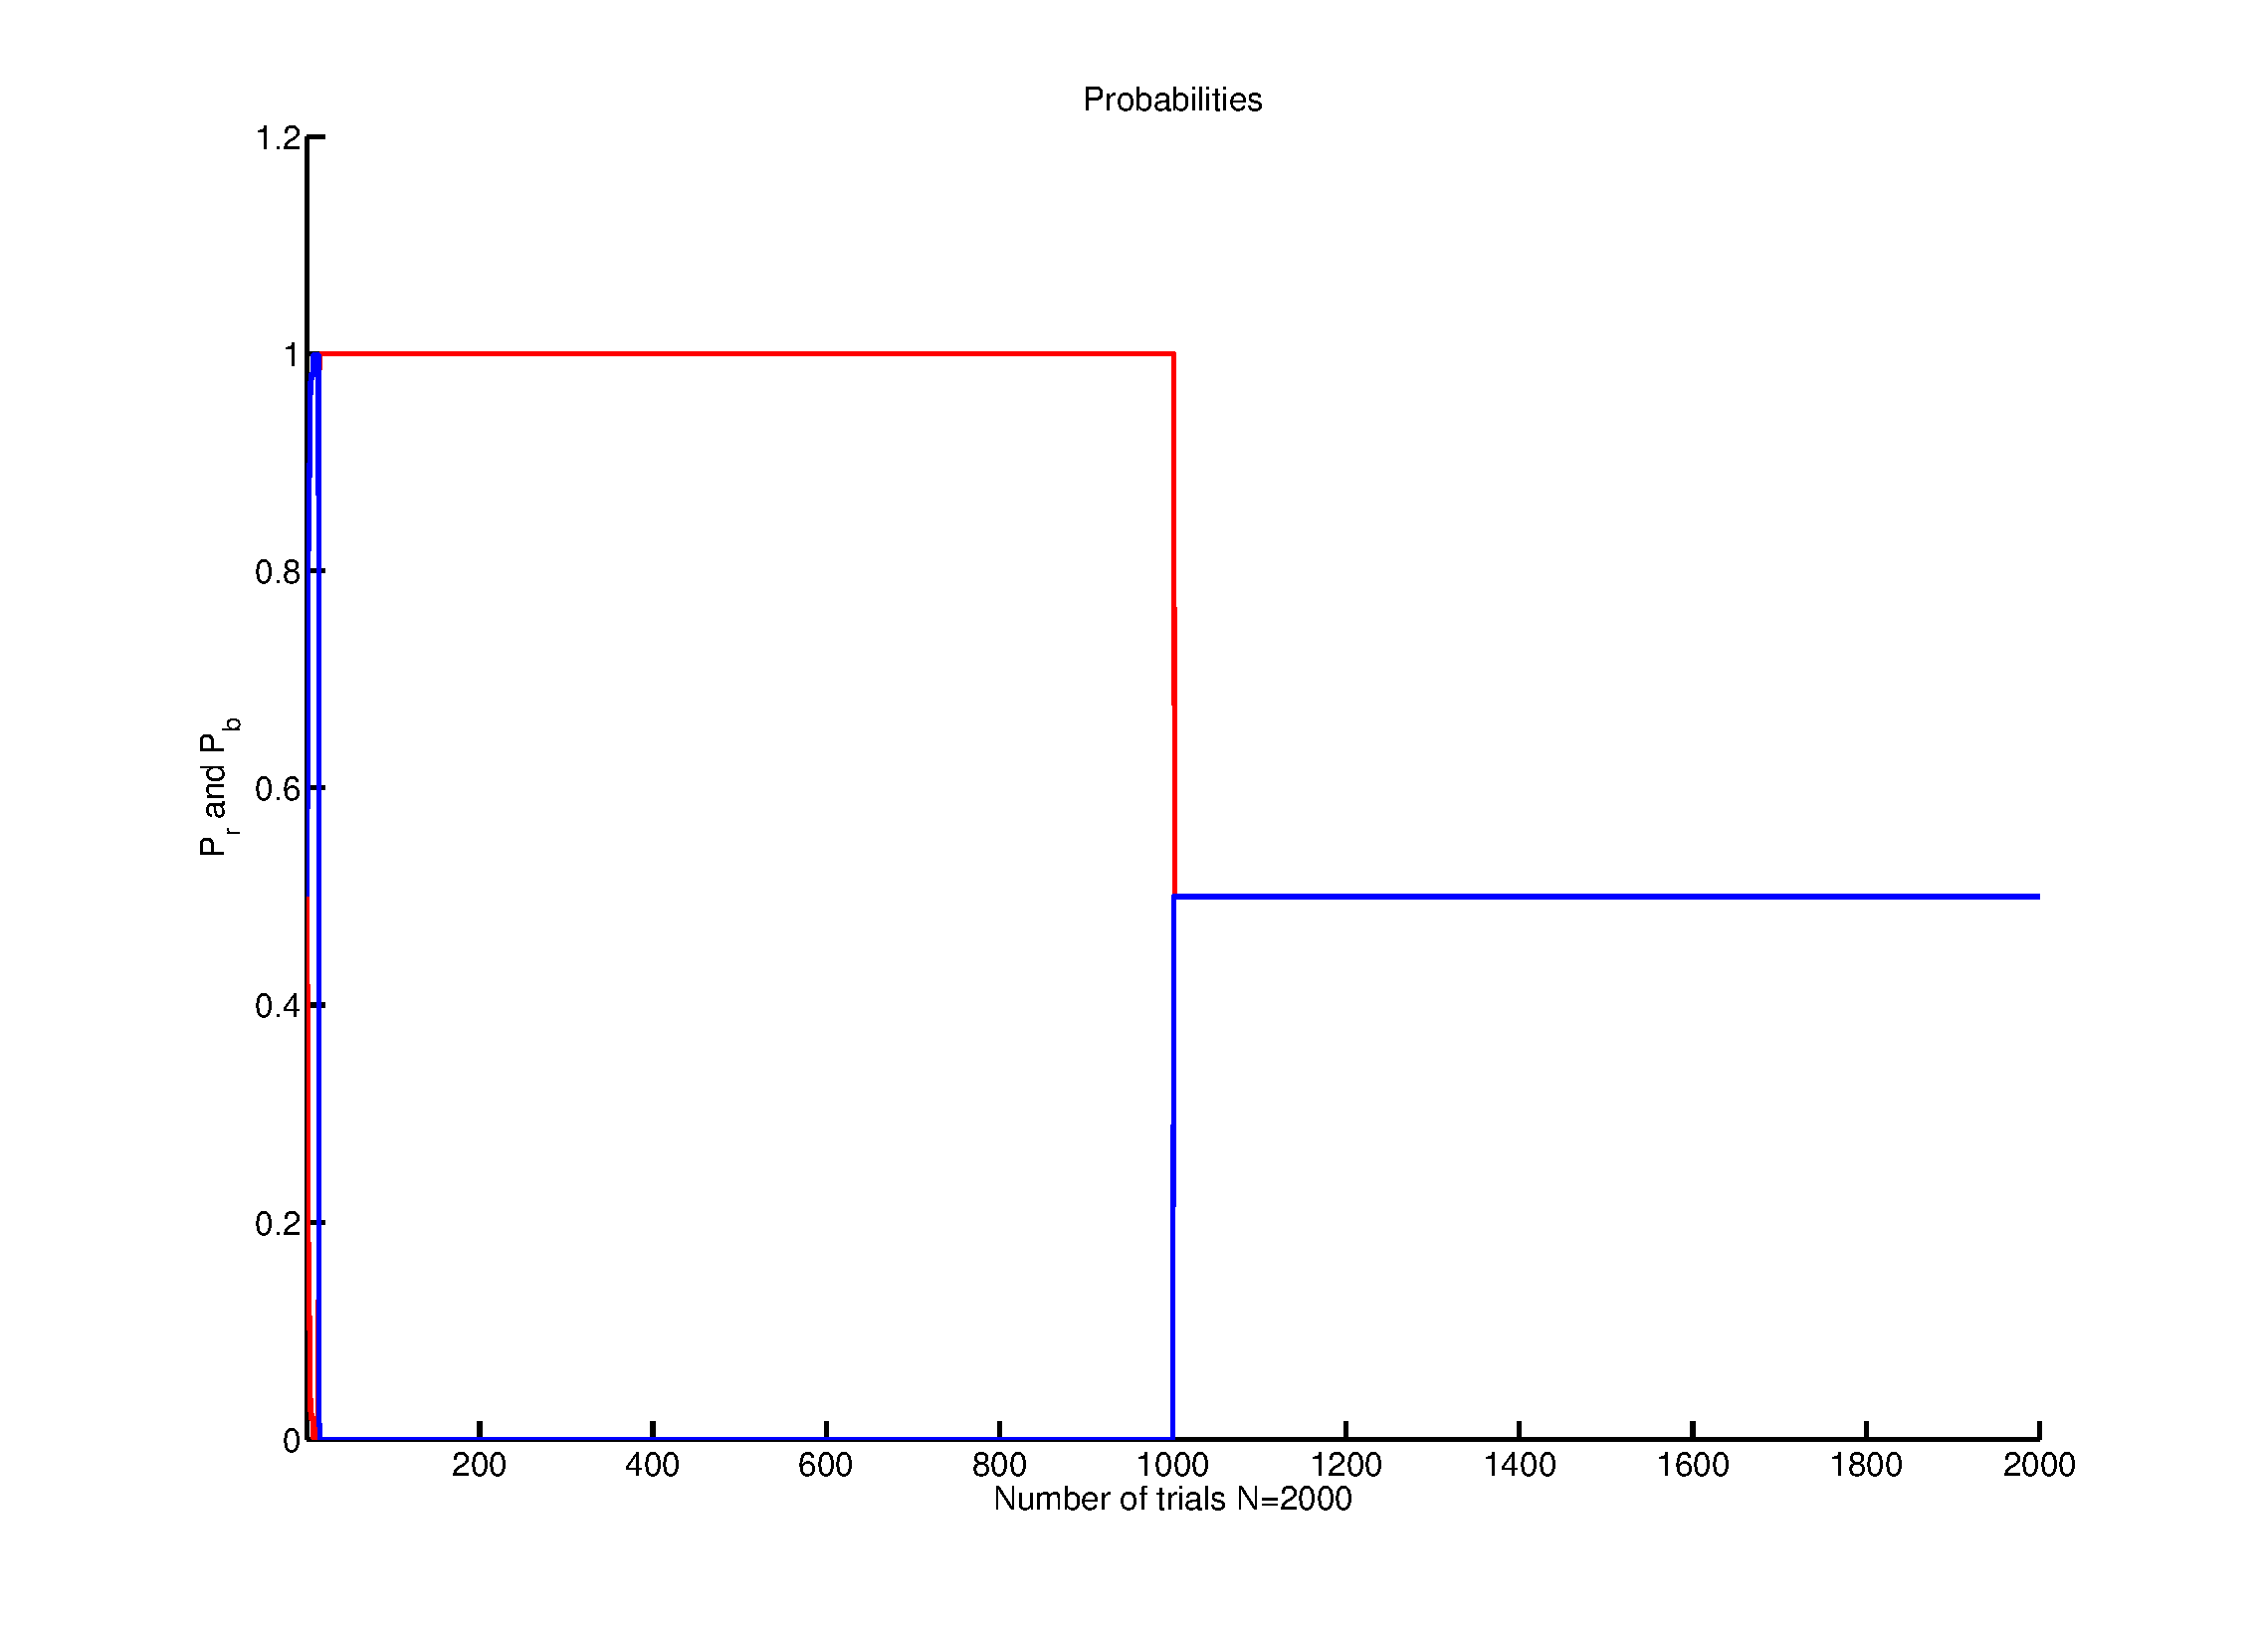
\includegraphics[width=\textwidth]{prob3.eps}
% tau4_M1.eps: 0x0 pixel, 300dpi, 0.00x0.00 cm, bb= -304   -42   918   834
\begin{footnotesize}
 Figure 8, $\beta=20$, $\epsilon=0.1$
\end{footnotesize}
\end{center}

\begin{center}
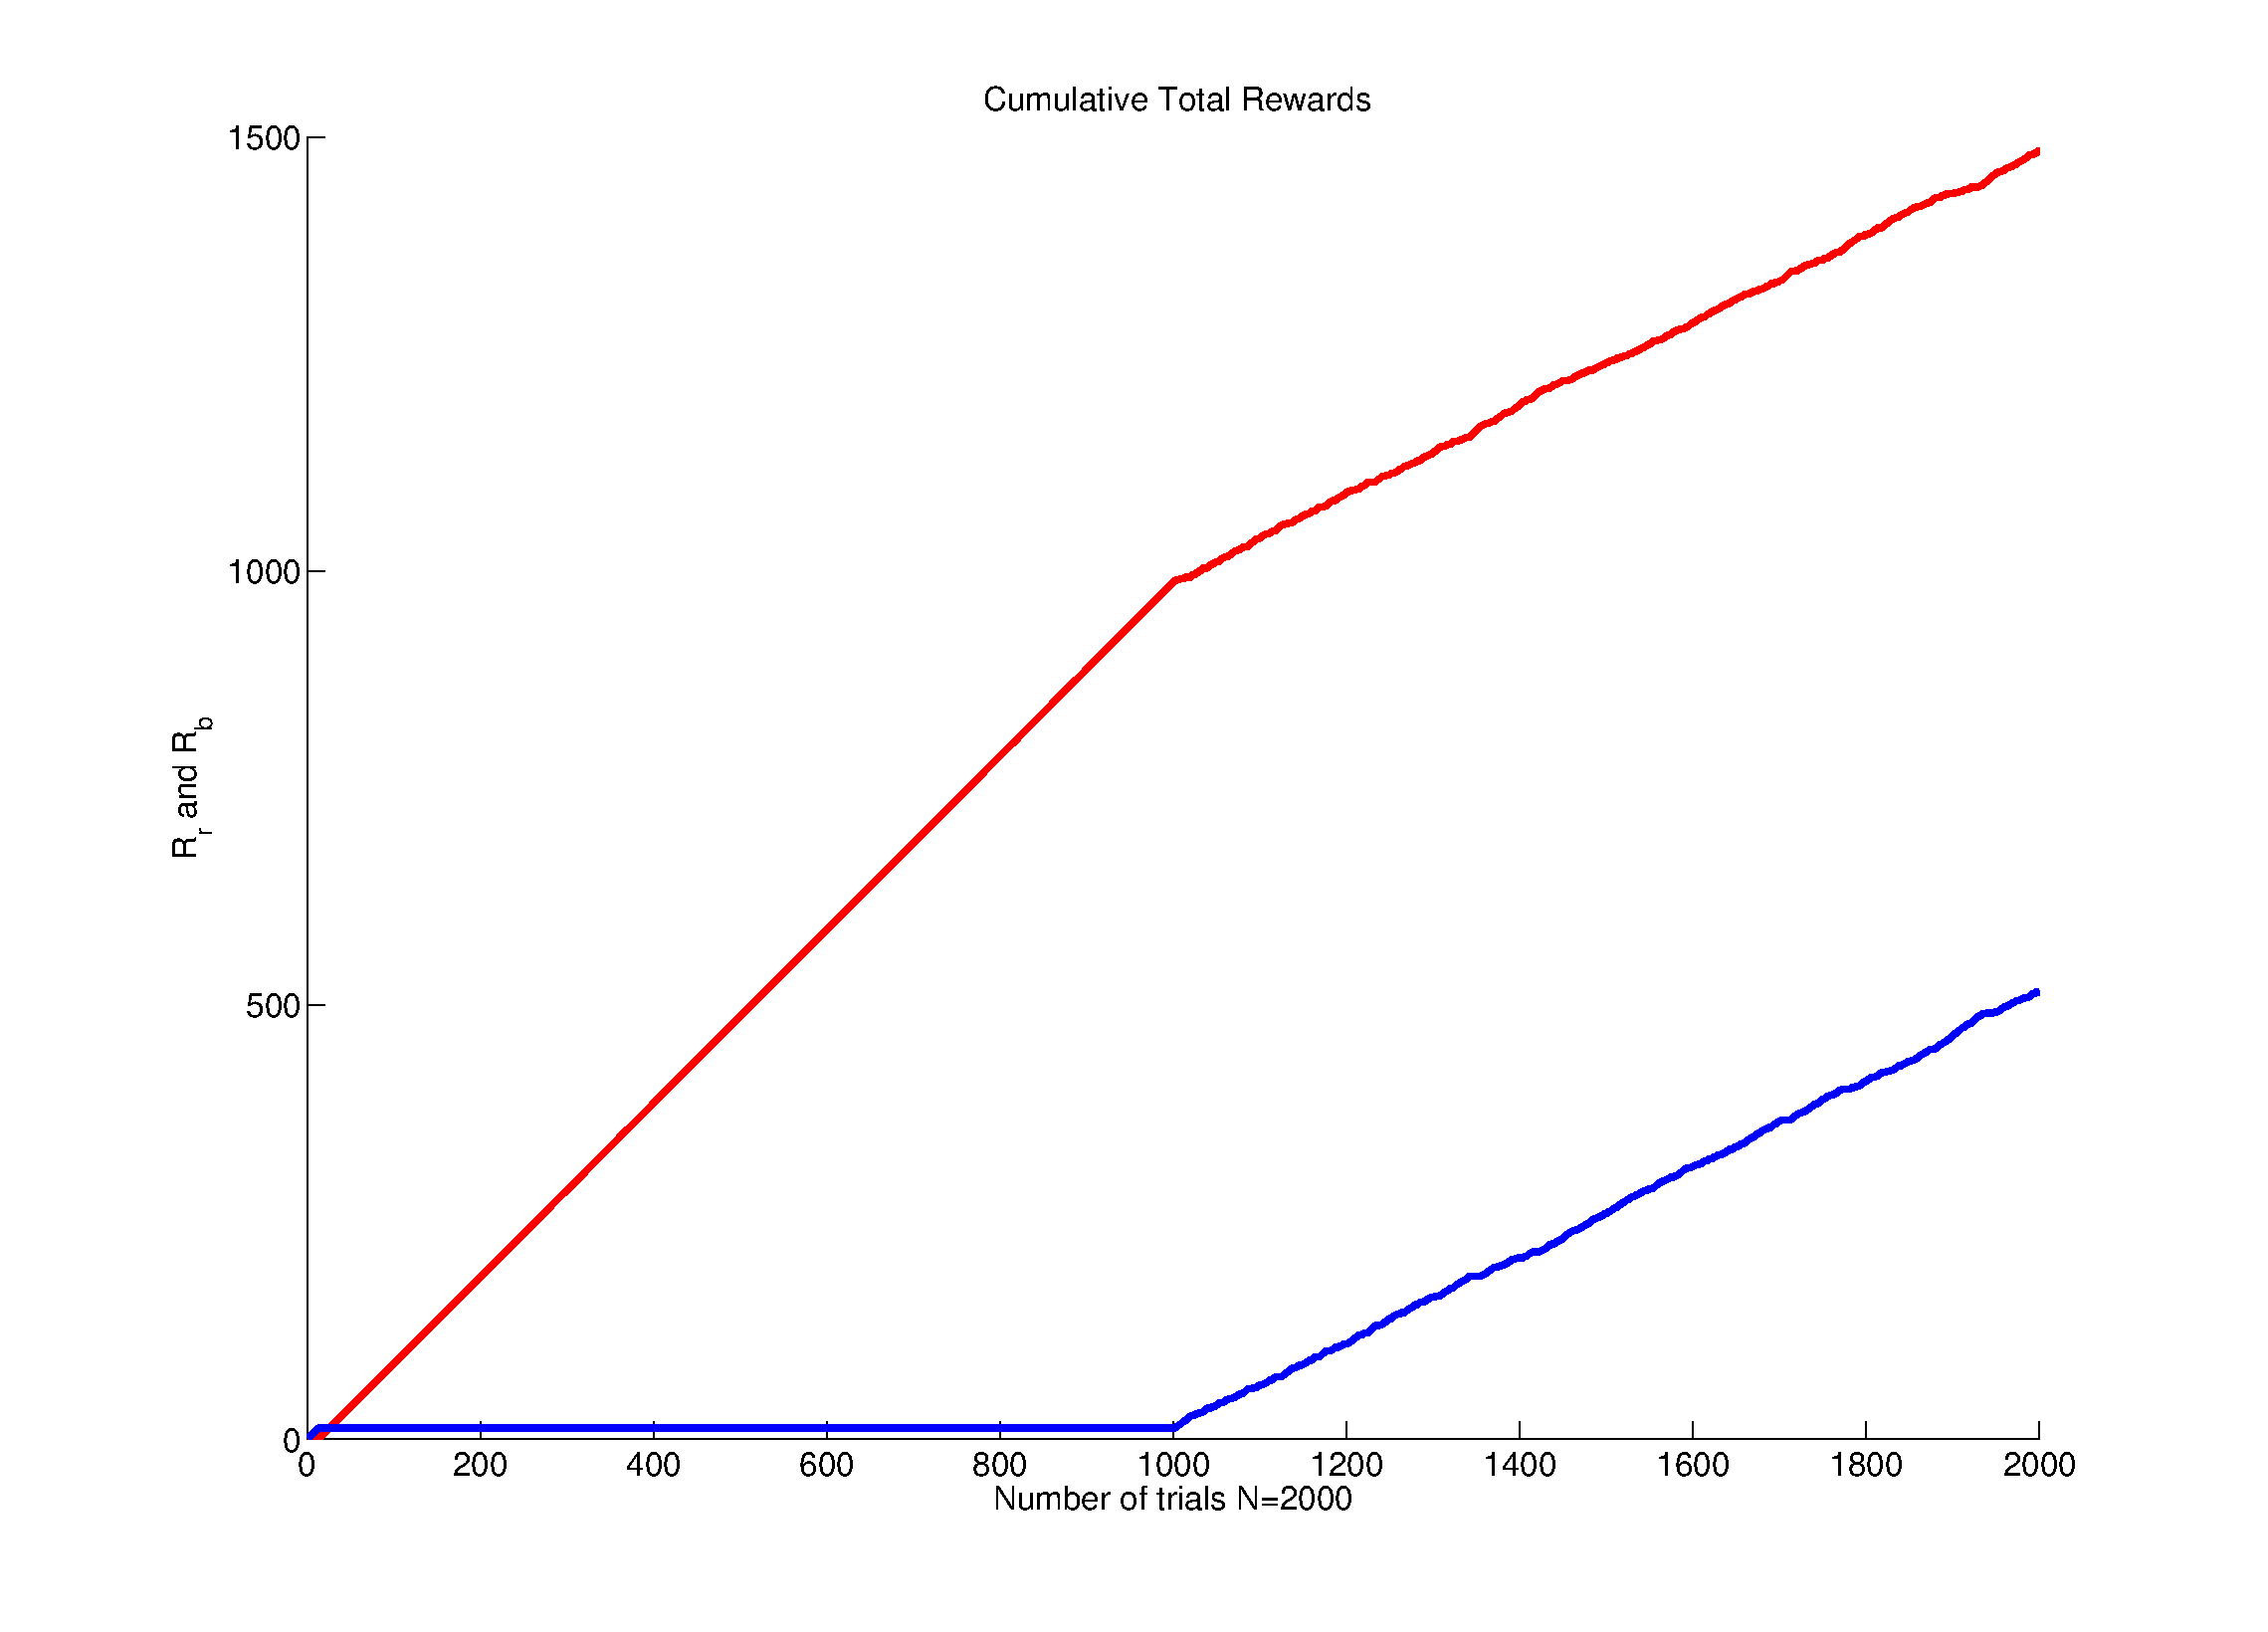
\includegraphics[width=\textwidth]{rew3.eps}
% tau4_M1.eps: 0x0 pixel, 300dpi, 0.00x0.00 cm, bb= -304   -42   918   834
\begin{footnotesize}
 Figure 9, $\beta=20$, $\epsilon=0.1$
\end{footnotesize}
\end{center}

\newpage
\begin{itemize}
 \item \textbf{ $\beta=20$, $\epsilon=10$}
\end{itemize}

\begin{center}
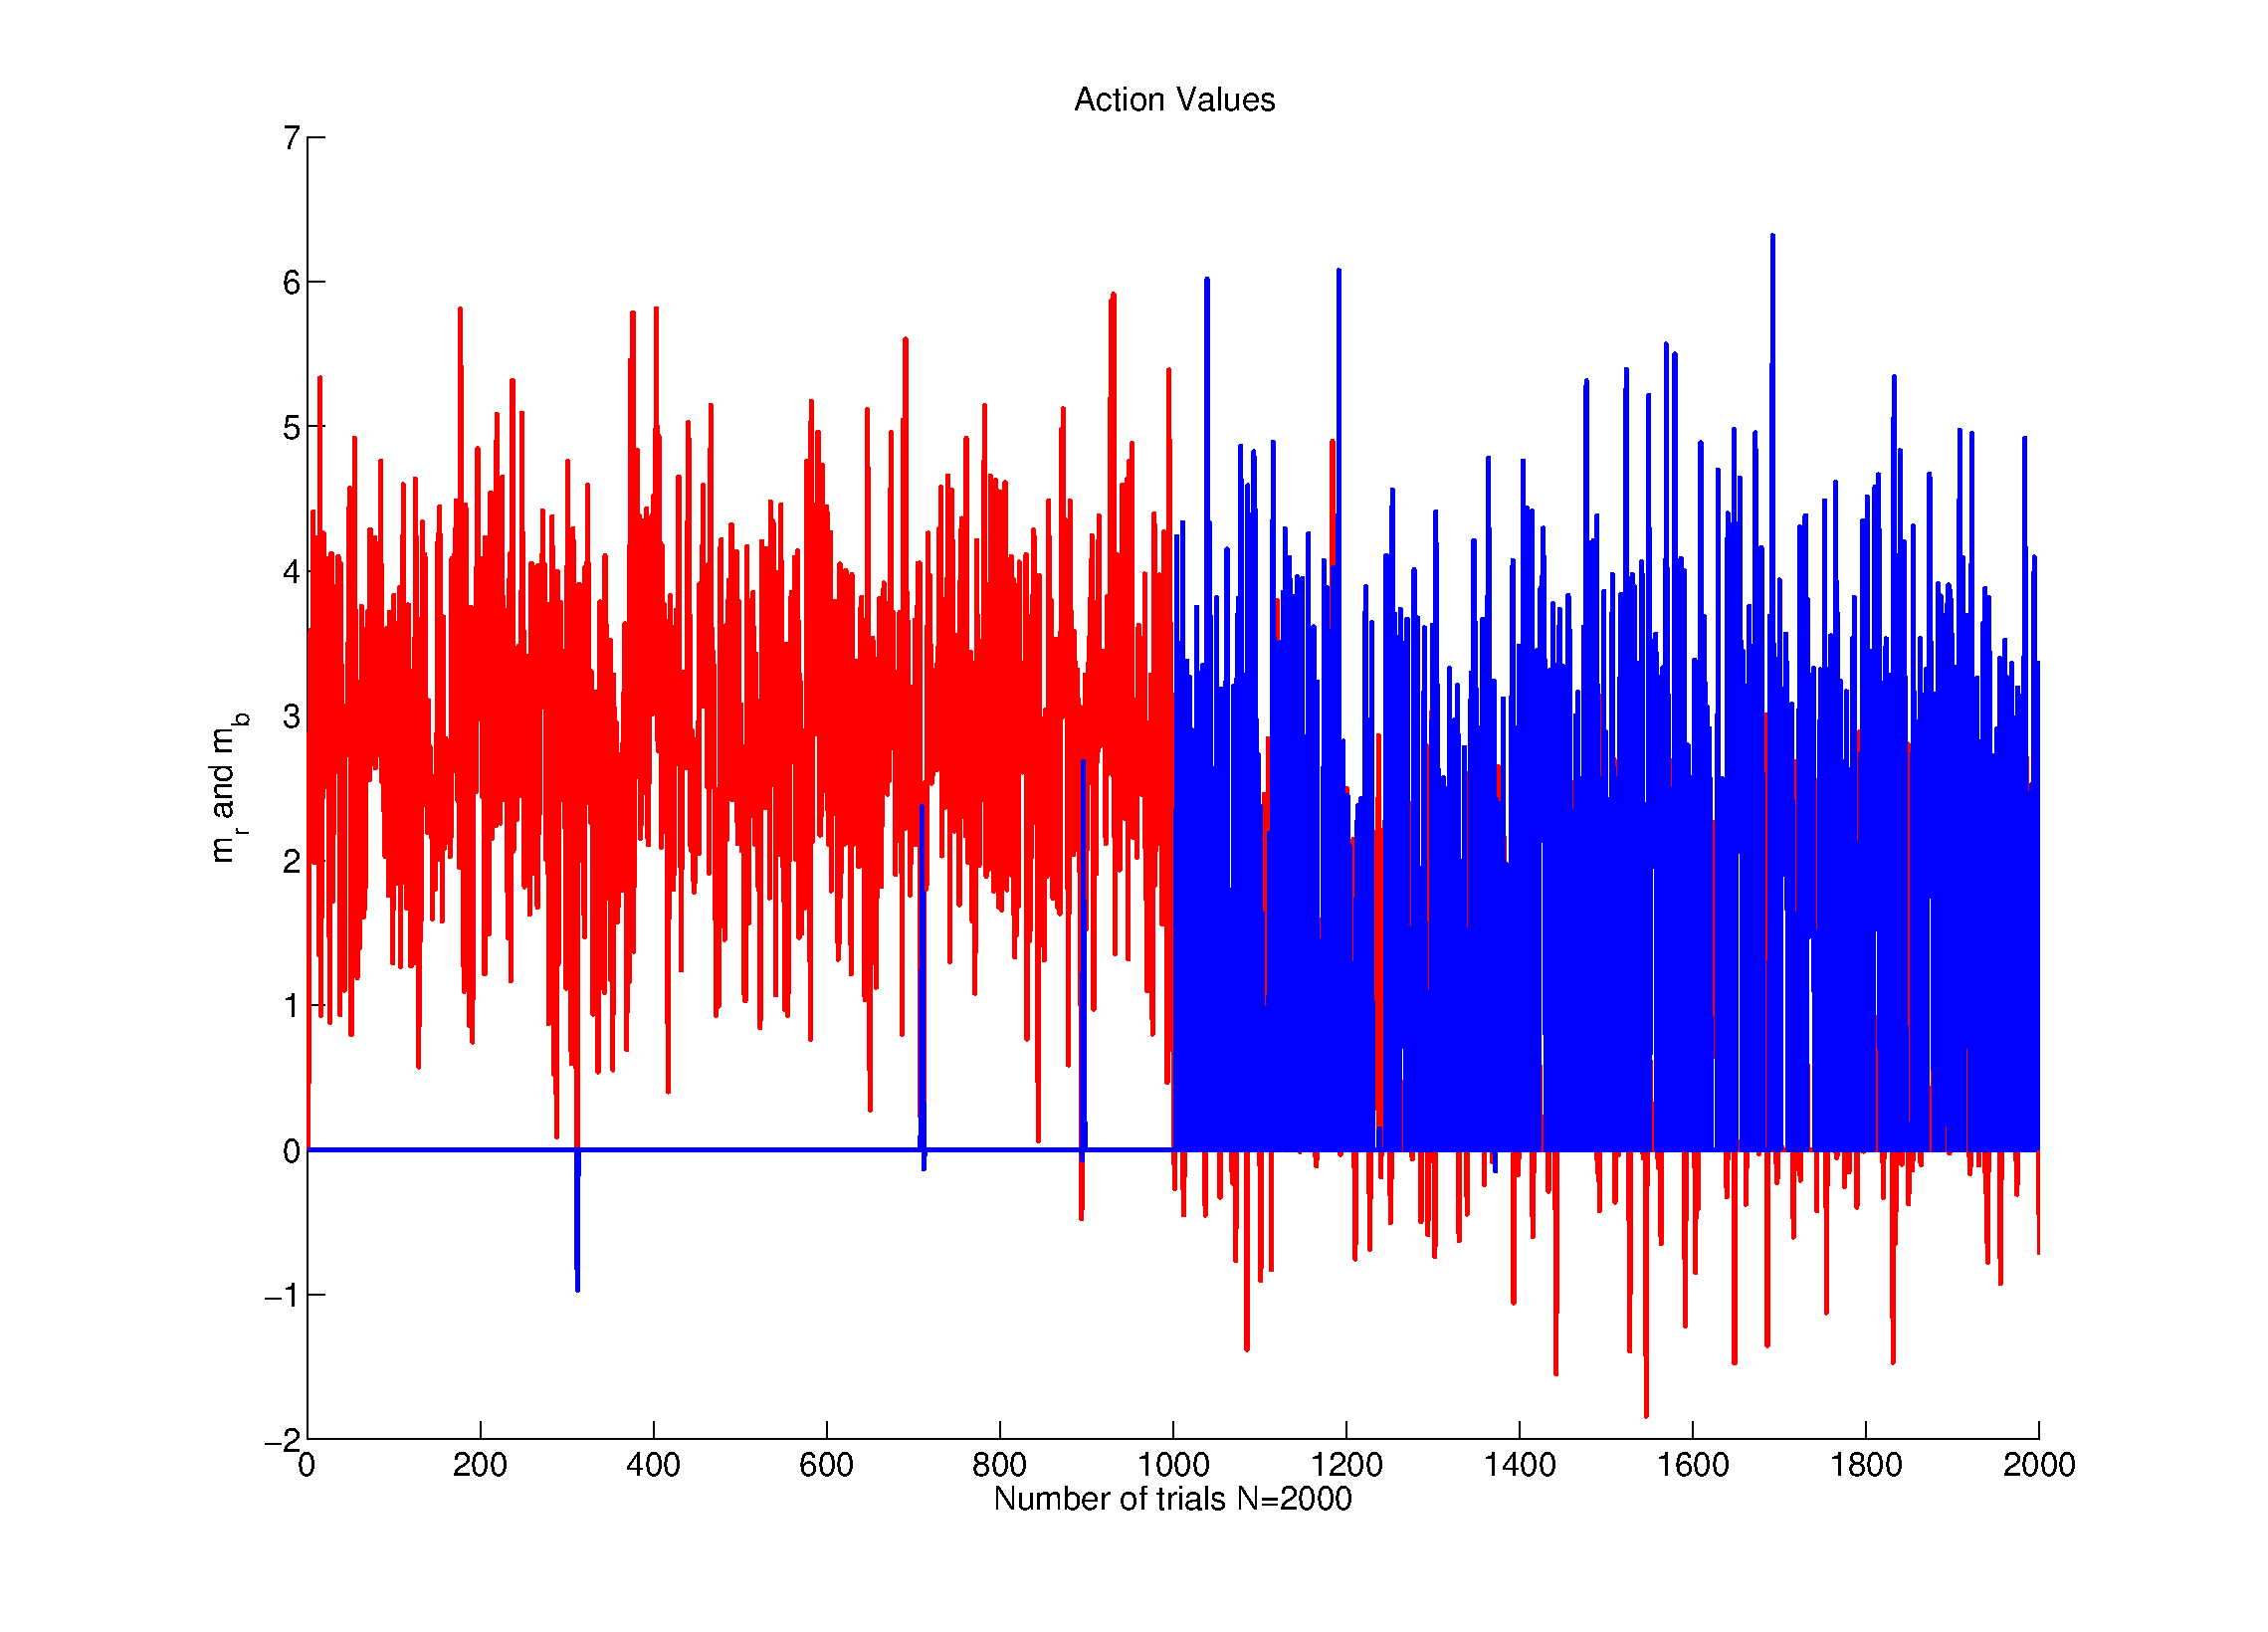
\includegraphics[width=\textwidth]{action4.eps}
% tau4_M1.eps: 0x0 pixel, 300dpi, 0.00x0.00 cm, bb= -304   -42   918   834
\begin{footnotesize}
 Figure 10, $\beta=20$, $\epsilon=10$
\end{footnotesize}
\end{center}

\begin{center}
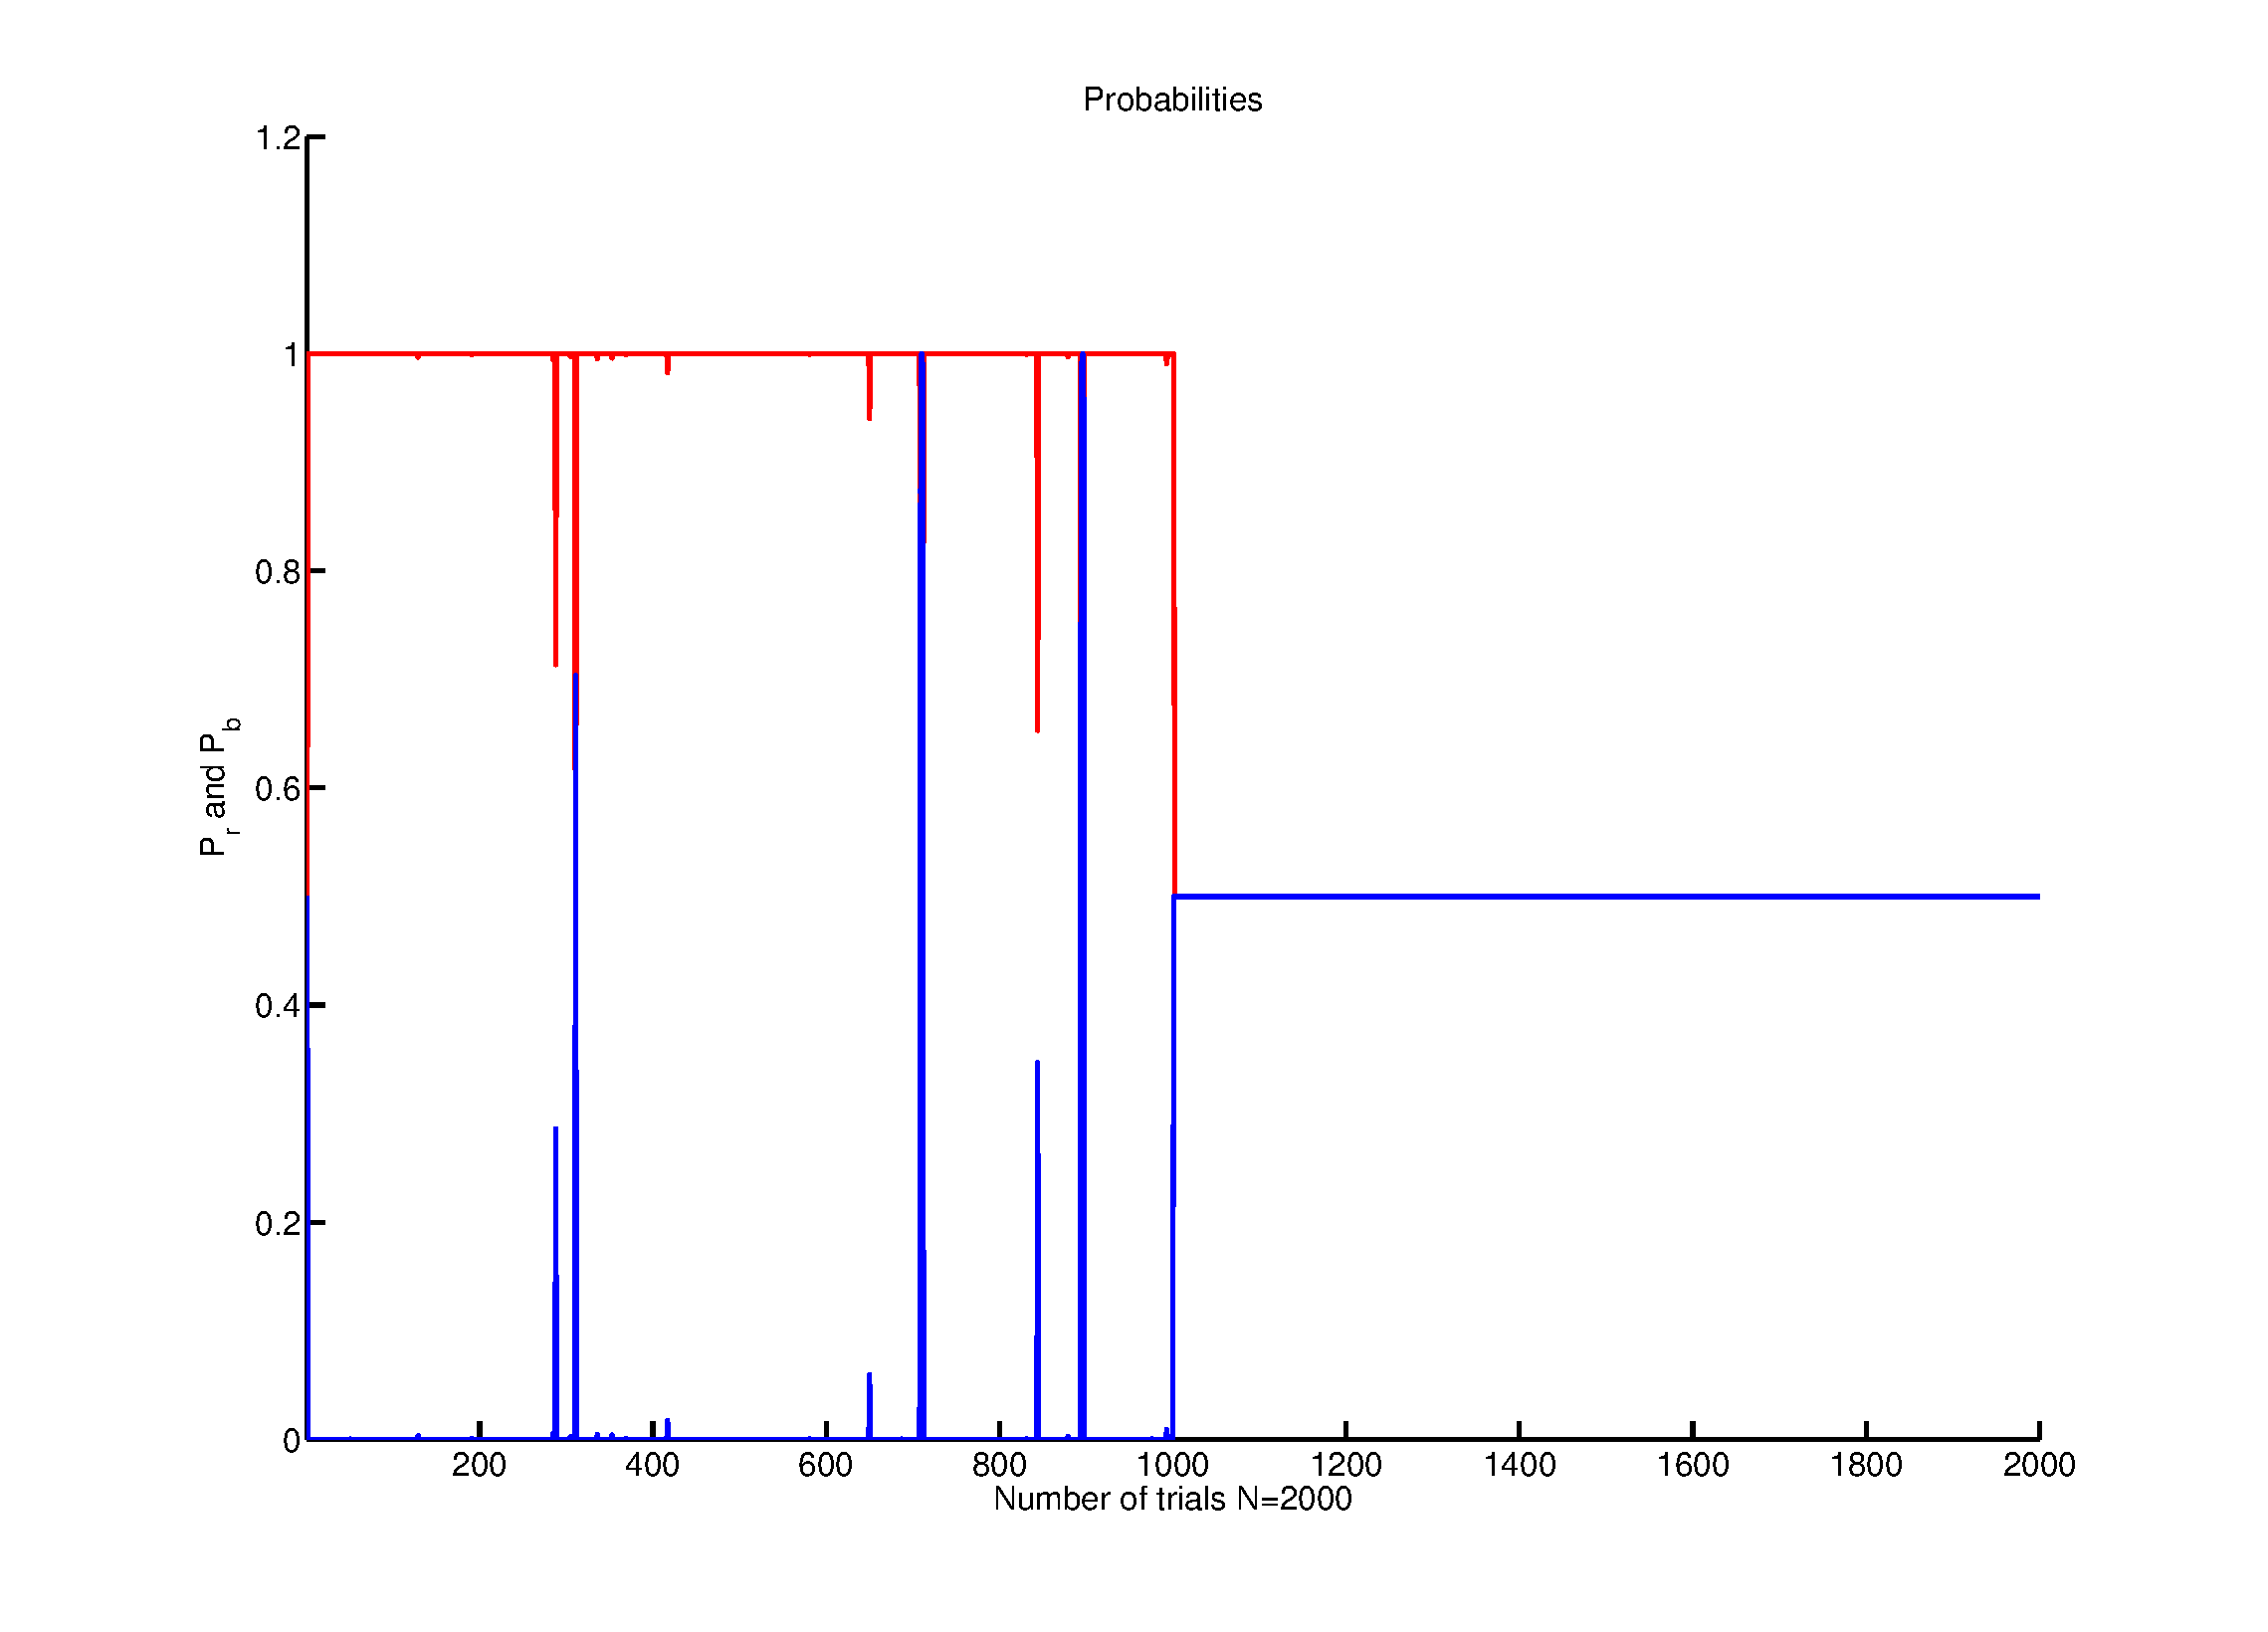
\includegraphics[width=\textwidth]{prob4.eps}
% tau4_M1.eps: 0x0 pixel, 300dpi, 0.00x0.00 cm, bb= -304   -42   918   834
\begin{footnotesize}
 Figure 11, $\beta=20$, $\epsilon=10$
\end{footnotesize}
\end{center}

\begin{center}
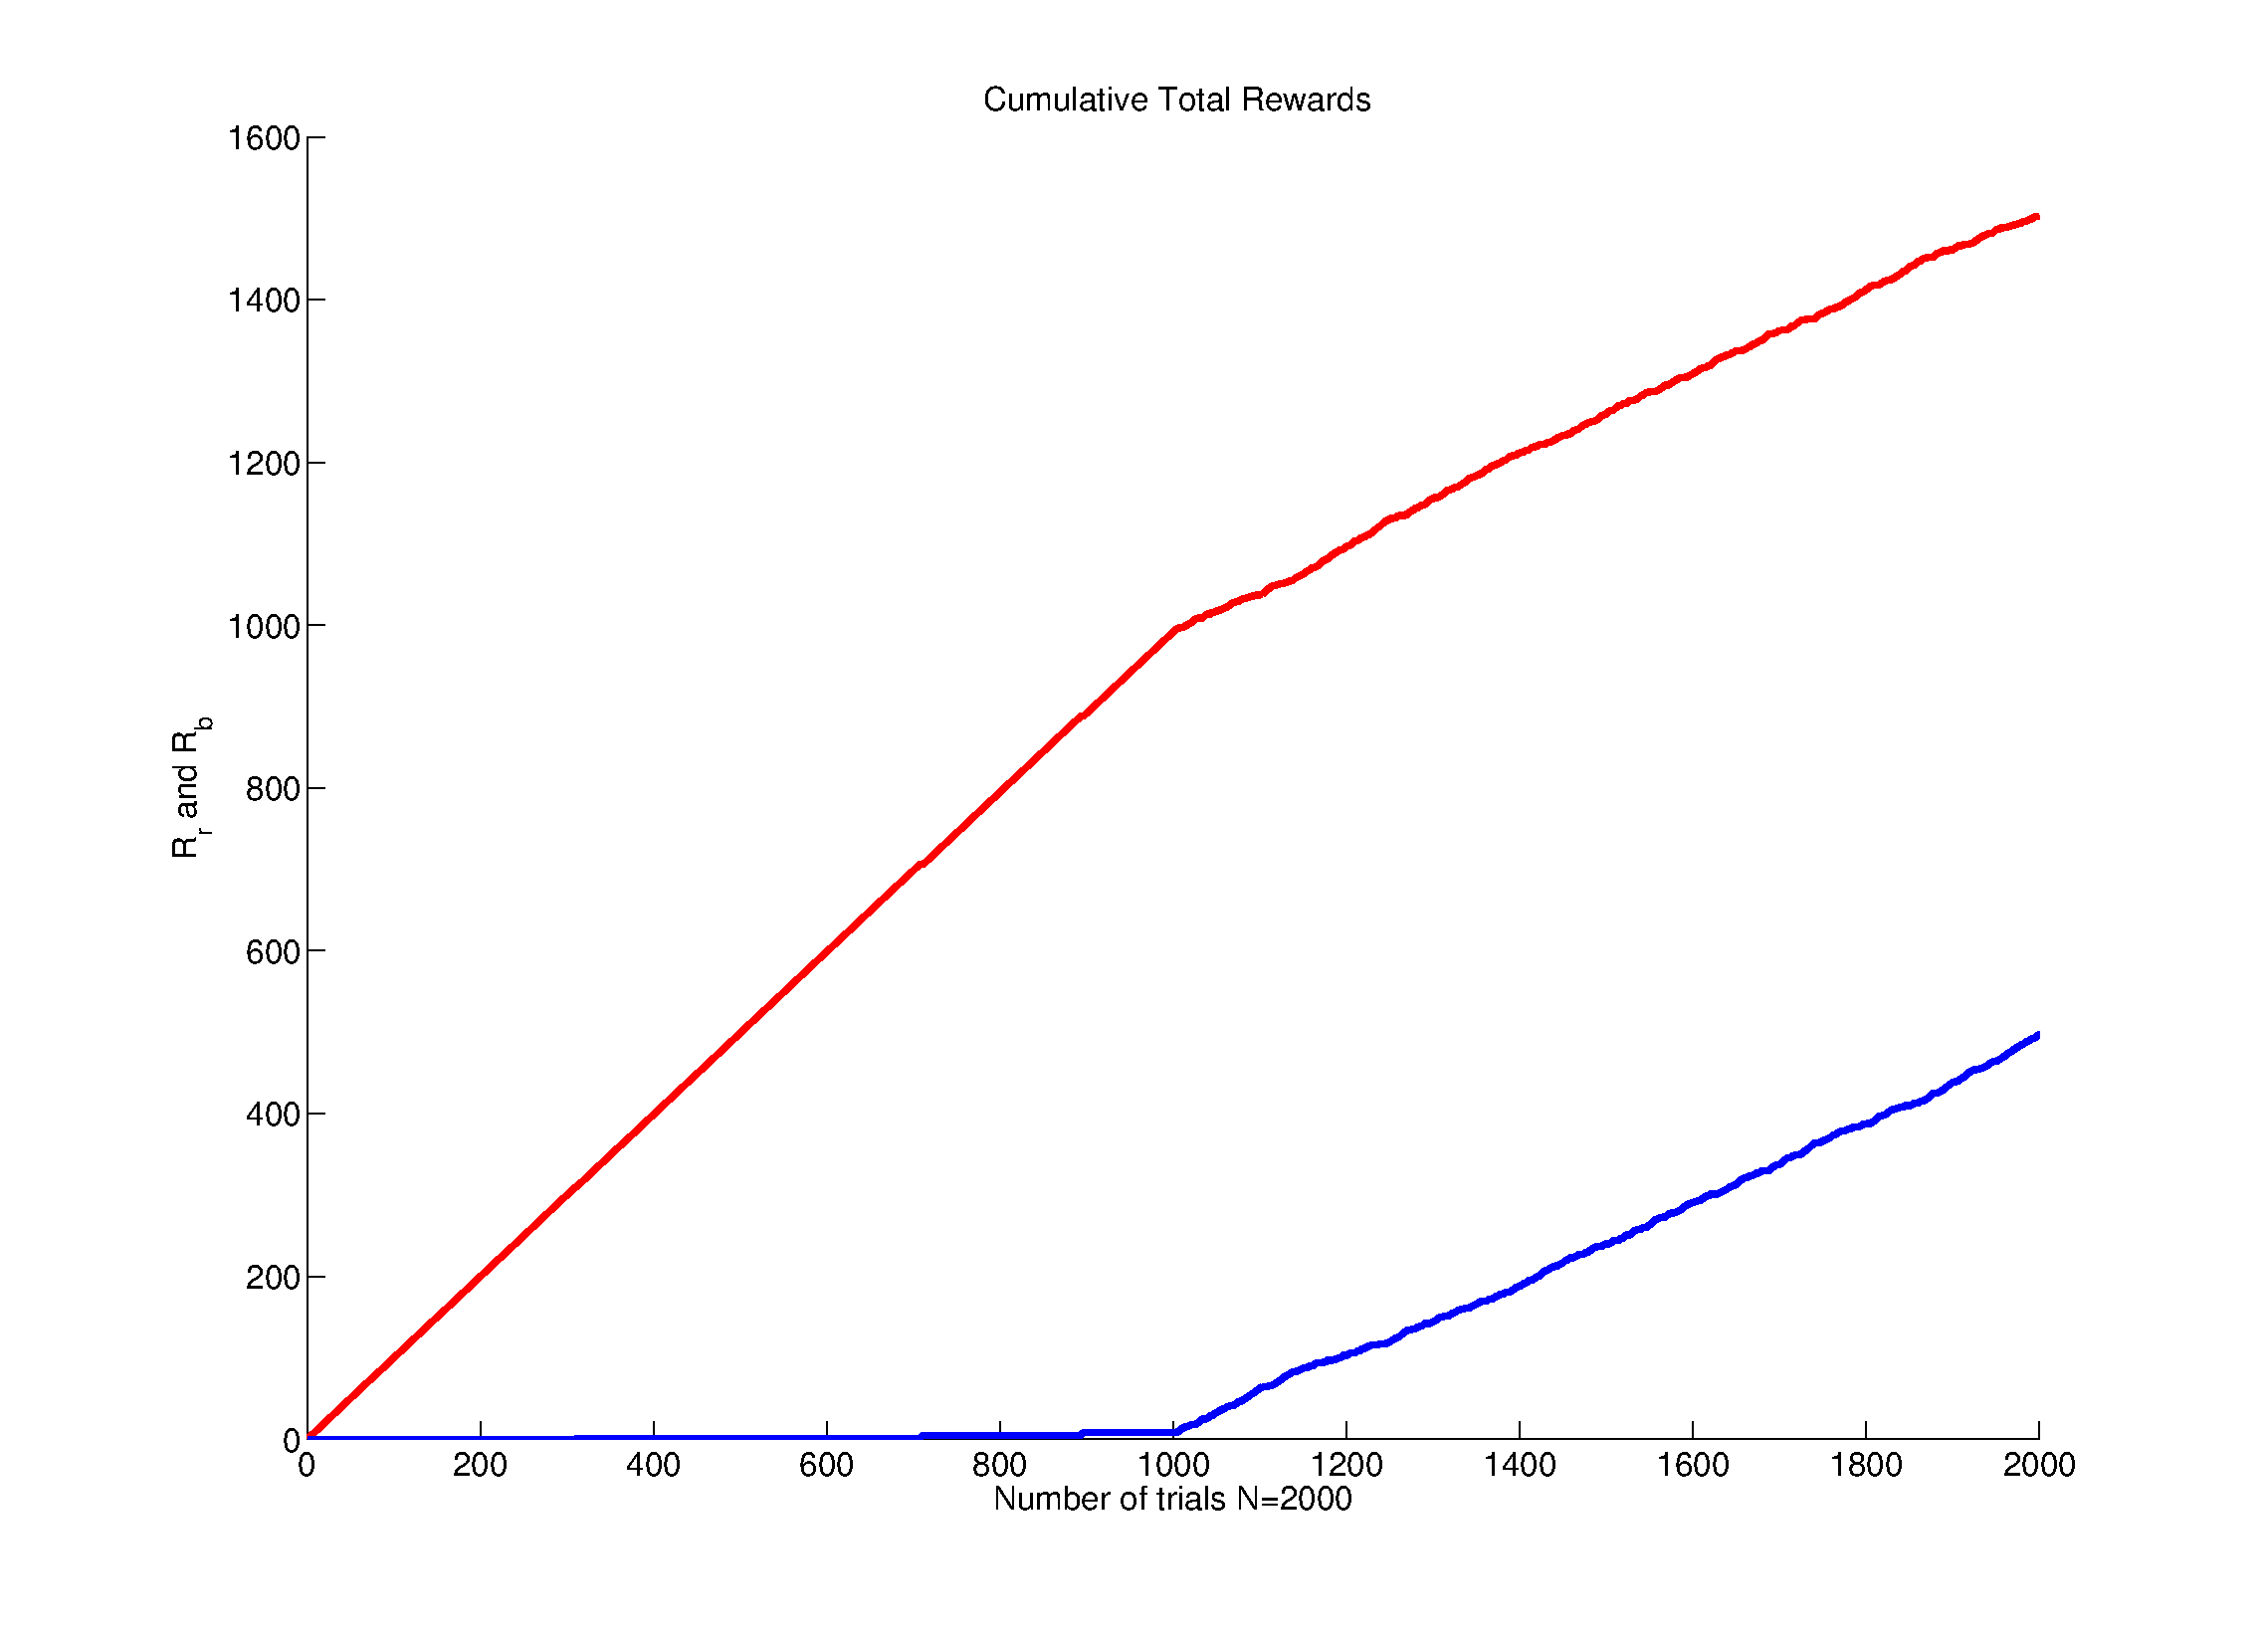
\includegraphics[width=\textwidth]{rew4.eps}
% tau4_M1.eps: 0x0 pixel, 300dpi, 0.00x0.00 cm, bb= -304   -42   918   834
\begin{footnotesize}
 Figure 12, $\beta=20$, $\epsilon=10$
\end{footnotesize}
\end{center}



\subsection{Discussion}
\begin{itemize}
 \item At first, the visits to the red flowers are rewarded more than the visits to the blue ones. Then this conditions was changed the other way around. The action values $m_r$ stays almost always above the $m_b$ in the first case for all $\beta$ values. However, the action value $m_b$ has been never observed as high as the $m_r$ in the second phase, even though the reward given to the blue flower was increased in the second phase. The system does not completely adjust itself to the newly assigned reward values in the second phase. It means that, the bee does not forget the previously learnt reward completely. 
\item When $\beta=2$, the learning is slow, when beta increases e.g. $\beta=20$, then the learning is well. Figure 6 shows that, a small $\beta$ value causes the bee to go to the blue flower more often in the first phase, even thought it is poorly rewarded. However, Figure 9 shows that, the bee learns faster to understand that the red flower is more awarded, so it goes almost all the time to the red one during the first phase. Whenever the reward is changed, the the bee starts also to go to the blue flower. The bee's visit to the blue flower in second phase is more in Figure 9 ($\beta=20$), in comparison to Figure 3 ($\beta=5$). The exploitation/exploration balance is controlled by $\beta$.
\item $\epsilon$ seems to play a role on controlling the fluctuation of visits or in other words the action values and also indirectly the probability values. The bigeer $\epsilon$ value brings more fluctuations to the action values and the probabilities as seen in Figure 11 and Figure 10. 
\item The probabilities always sum to 1; $P_r+P_b=1$. However, when $\beta$ is small, then the probability to visit the blue flower int the first phase seems to increase, Figure 5. In the second phase, $P_t$ seems to increase in comparison to the first phase, but this incremant is a constant, it never becomes as high as $P_b$ in the first phase.
\end{itemize}

\section{Direct Actor}

The initial values of $m_b$ and $m_r$ are again assigned to 0, but this time their evaluation are changed as the following:


\textbf{Chose Red:}
\begin{equation*}
 m_r\rightarrow m_r + \epsilon (1-P_r)(r_r-{\bar r})  \;\;\;\;\;\;\; m_b\rightarrow m_b - \epsilon P_b(r_r-{\bar r}) 
\end{equation*}

\textbf{Chose Blue:}
\begin{equation*}
 m_b\rightarrow m_b + \epsilon (1-P_b)(r_b-{\bar r})  \;\;\;\;\;\;\; m_r\rightarrow m_r - \epsilon P_r(r_b-{\bar r}) 
\end{equation*}
where ${\bar r}=\frac{1}{2}(\langle r_b\rangle + \langle r_r\rangle)$ is the mean collected reward.

\subsection{Programming Assignment for Direct Actor}

\begin{itemize}
 \item \textbf{ $\beta=2$, $\epsilon=0.1$}
\end{itemize}

\begin{center}
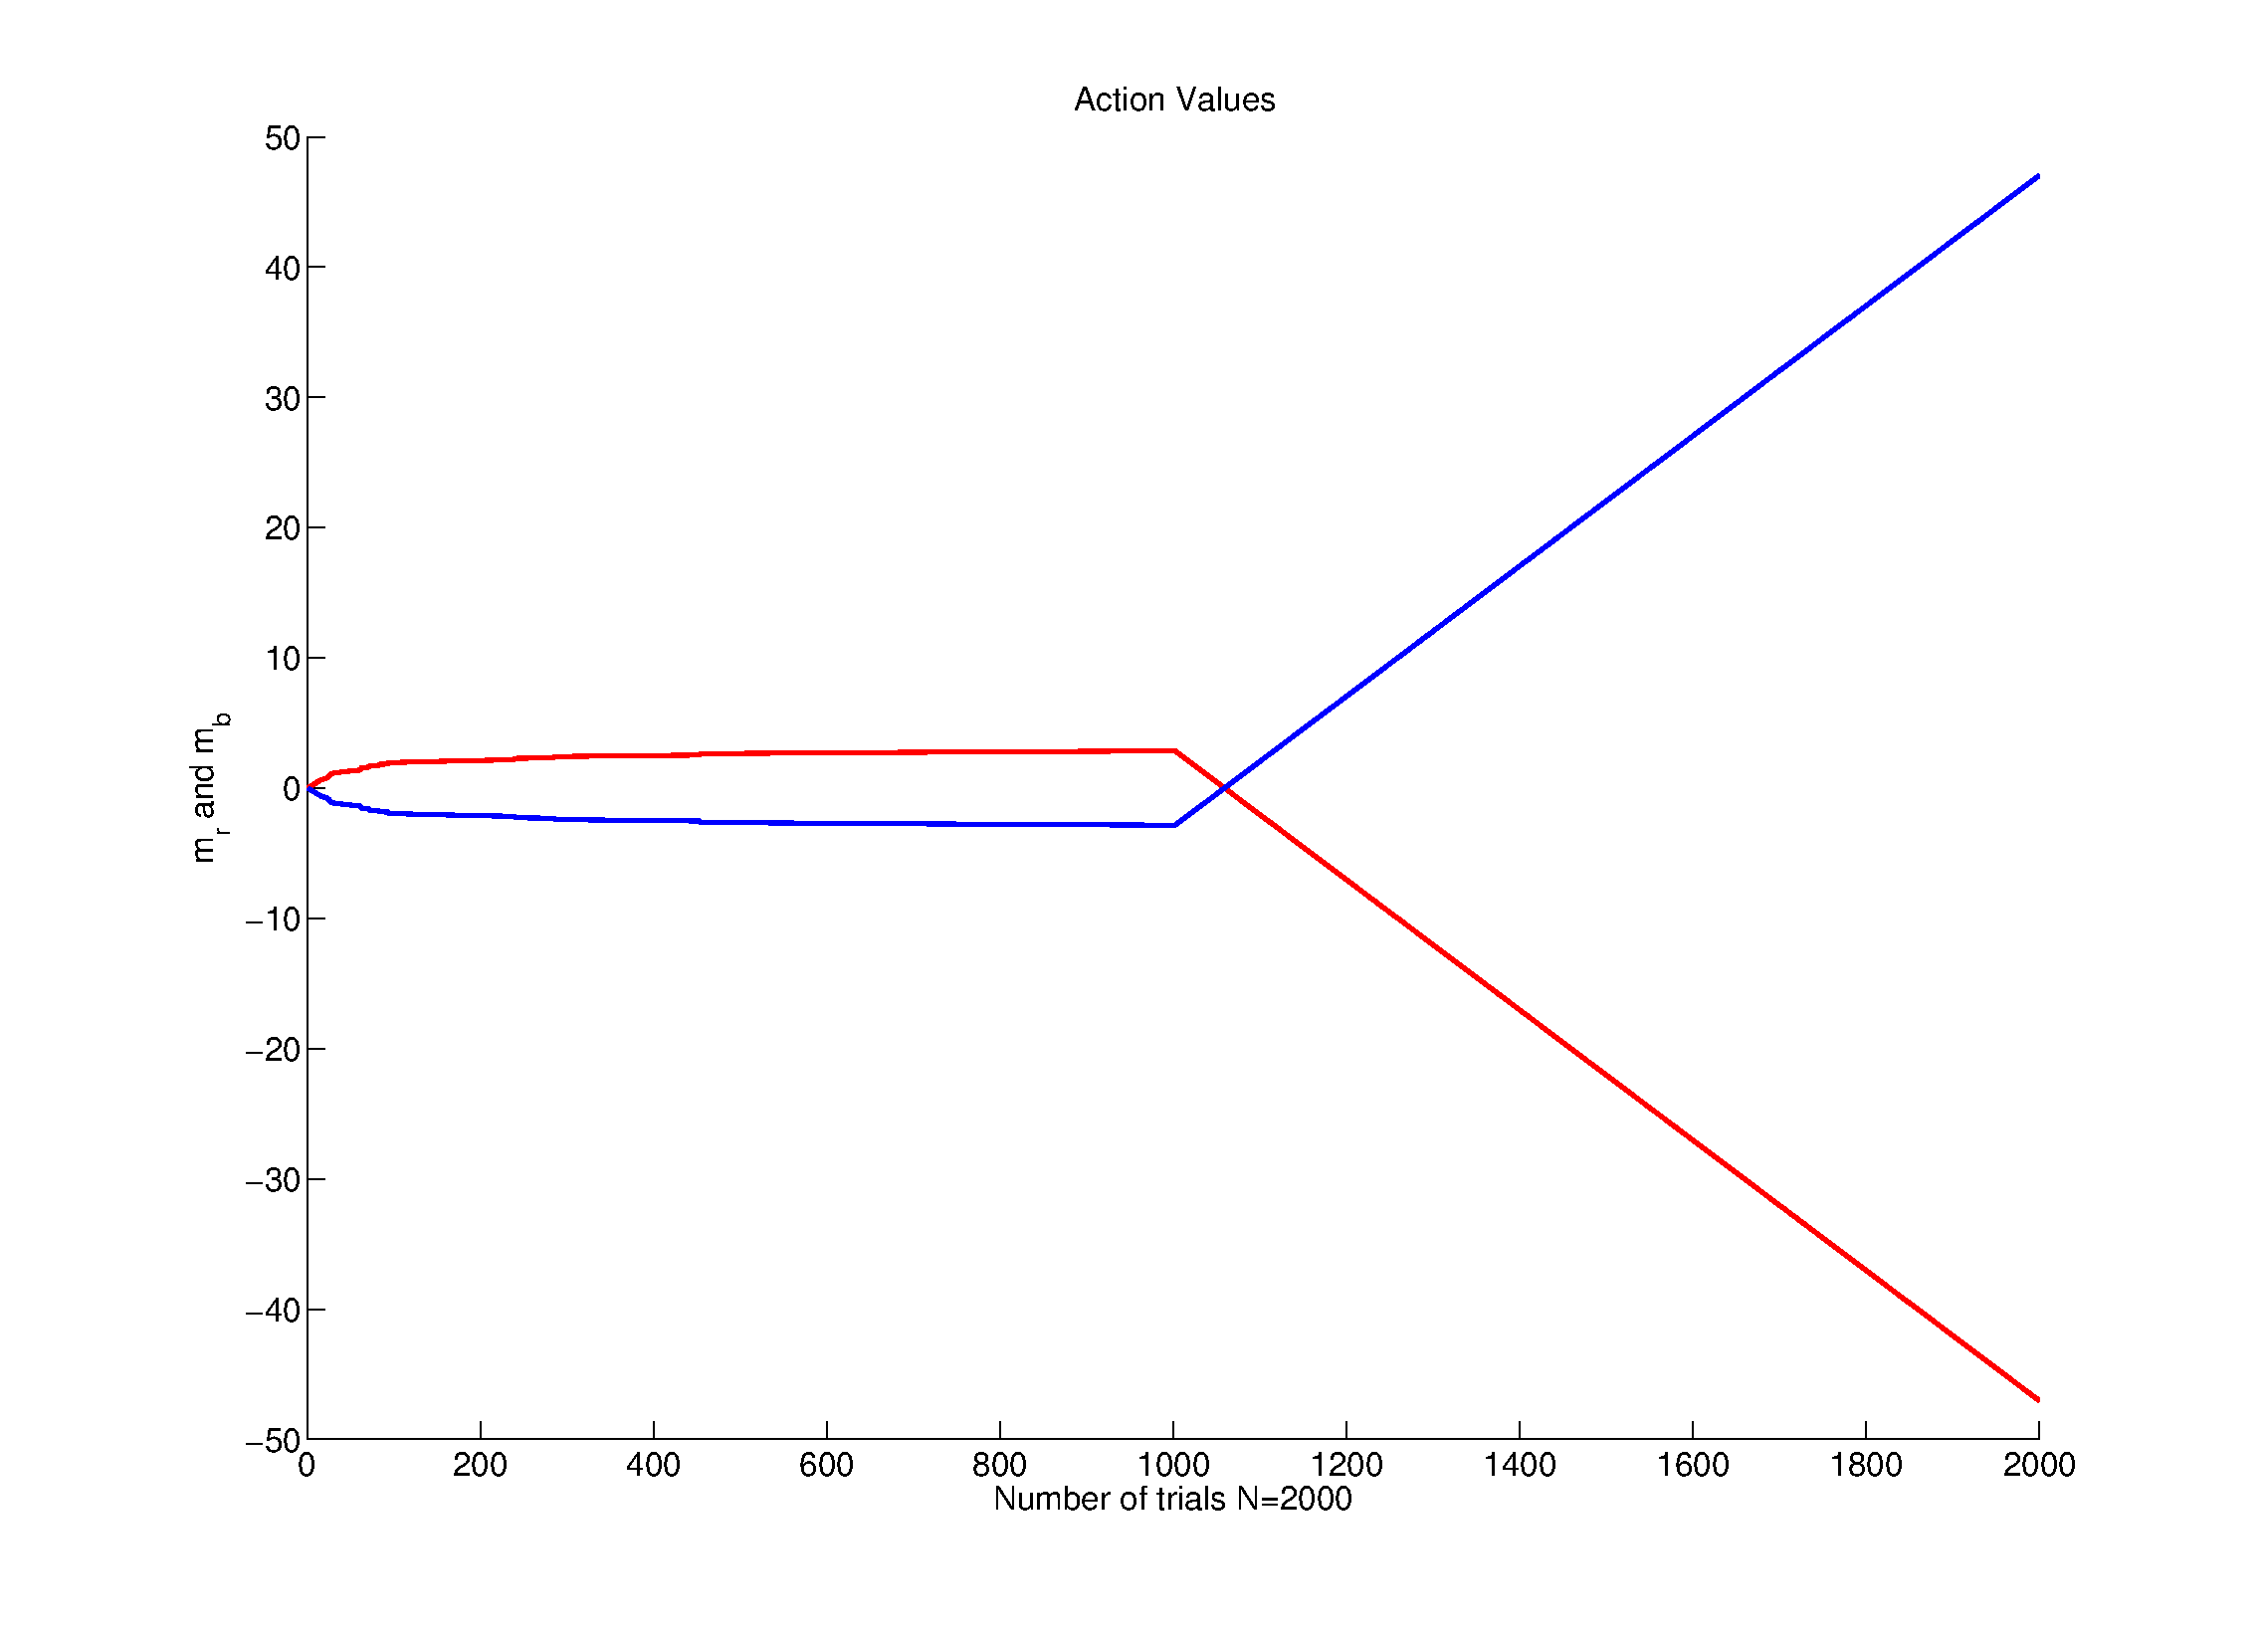
\includegraphics[width=\textwidth, height=80mm]{d_action1.eps}
% tau4_M1.eps: 0x0 pixel, 300dpi, 0.00x0.00 cm, bb= -304   -42   918   834
\begin{footnotesize}
 Figure 13, $\beta=2$, $\epsilon=0.1$
\end{footnotesize}
\end{center}

\begin{center}
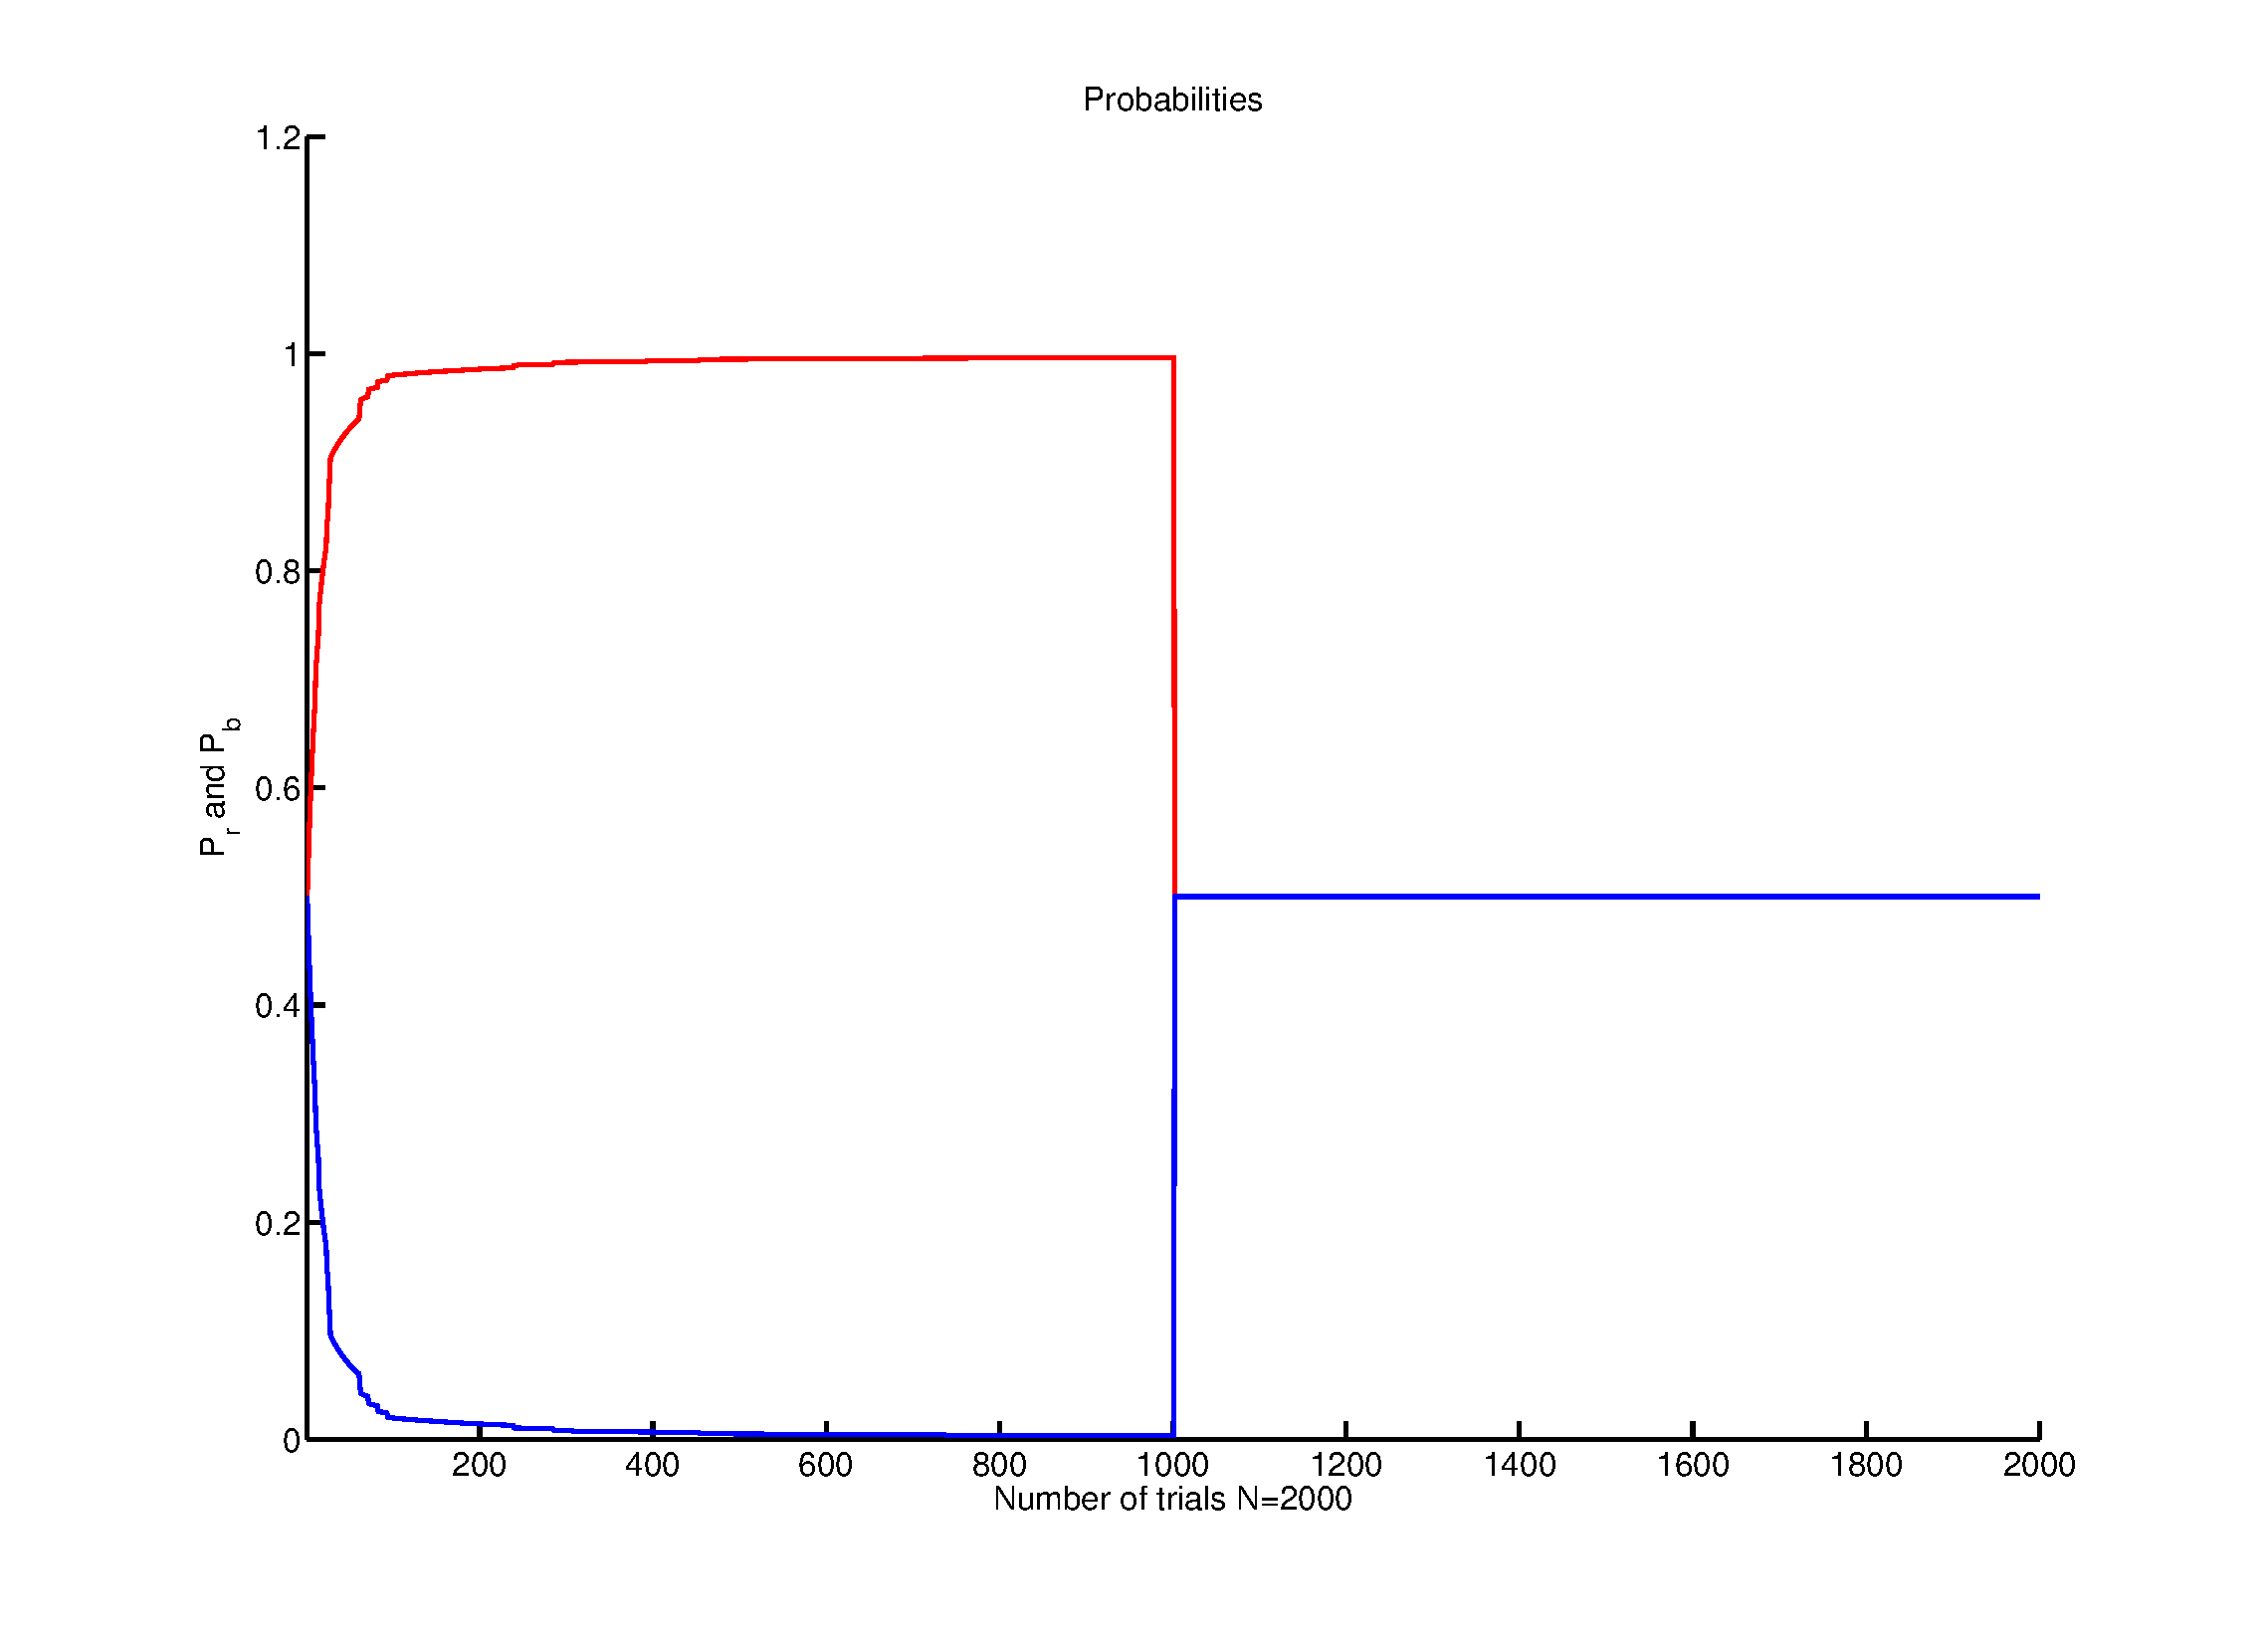
\includegraphics[width=\textwidth]{d_prob1.eps}
% tau4_M1.eps: 0x0 pixel, 300dpi, 0.00x0.00 cm, bb= -304   -42   918   834
\begin{footnotesize}
 Figure 14, $\beta=2$, $\epsilon=0.1$
\end{footnotesize}
\end{center}

\begin{center}
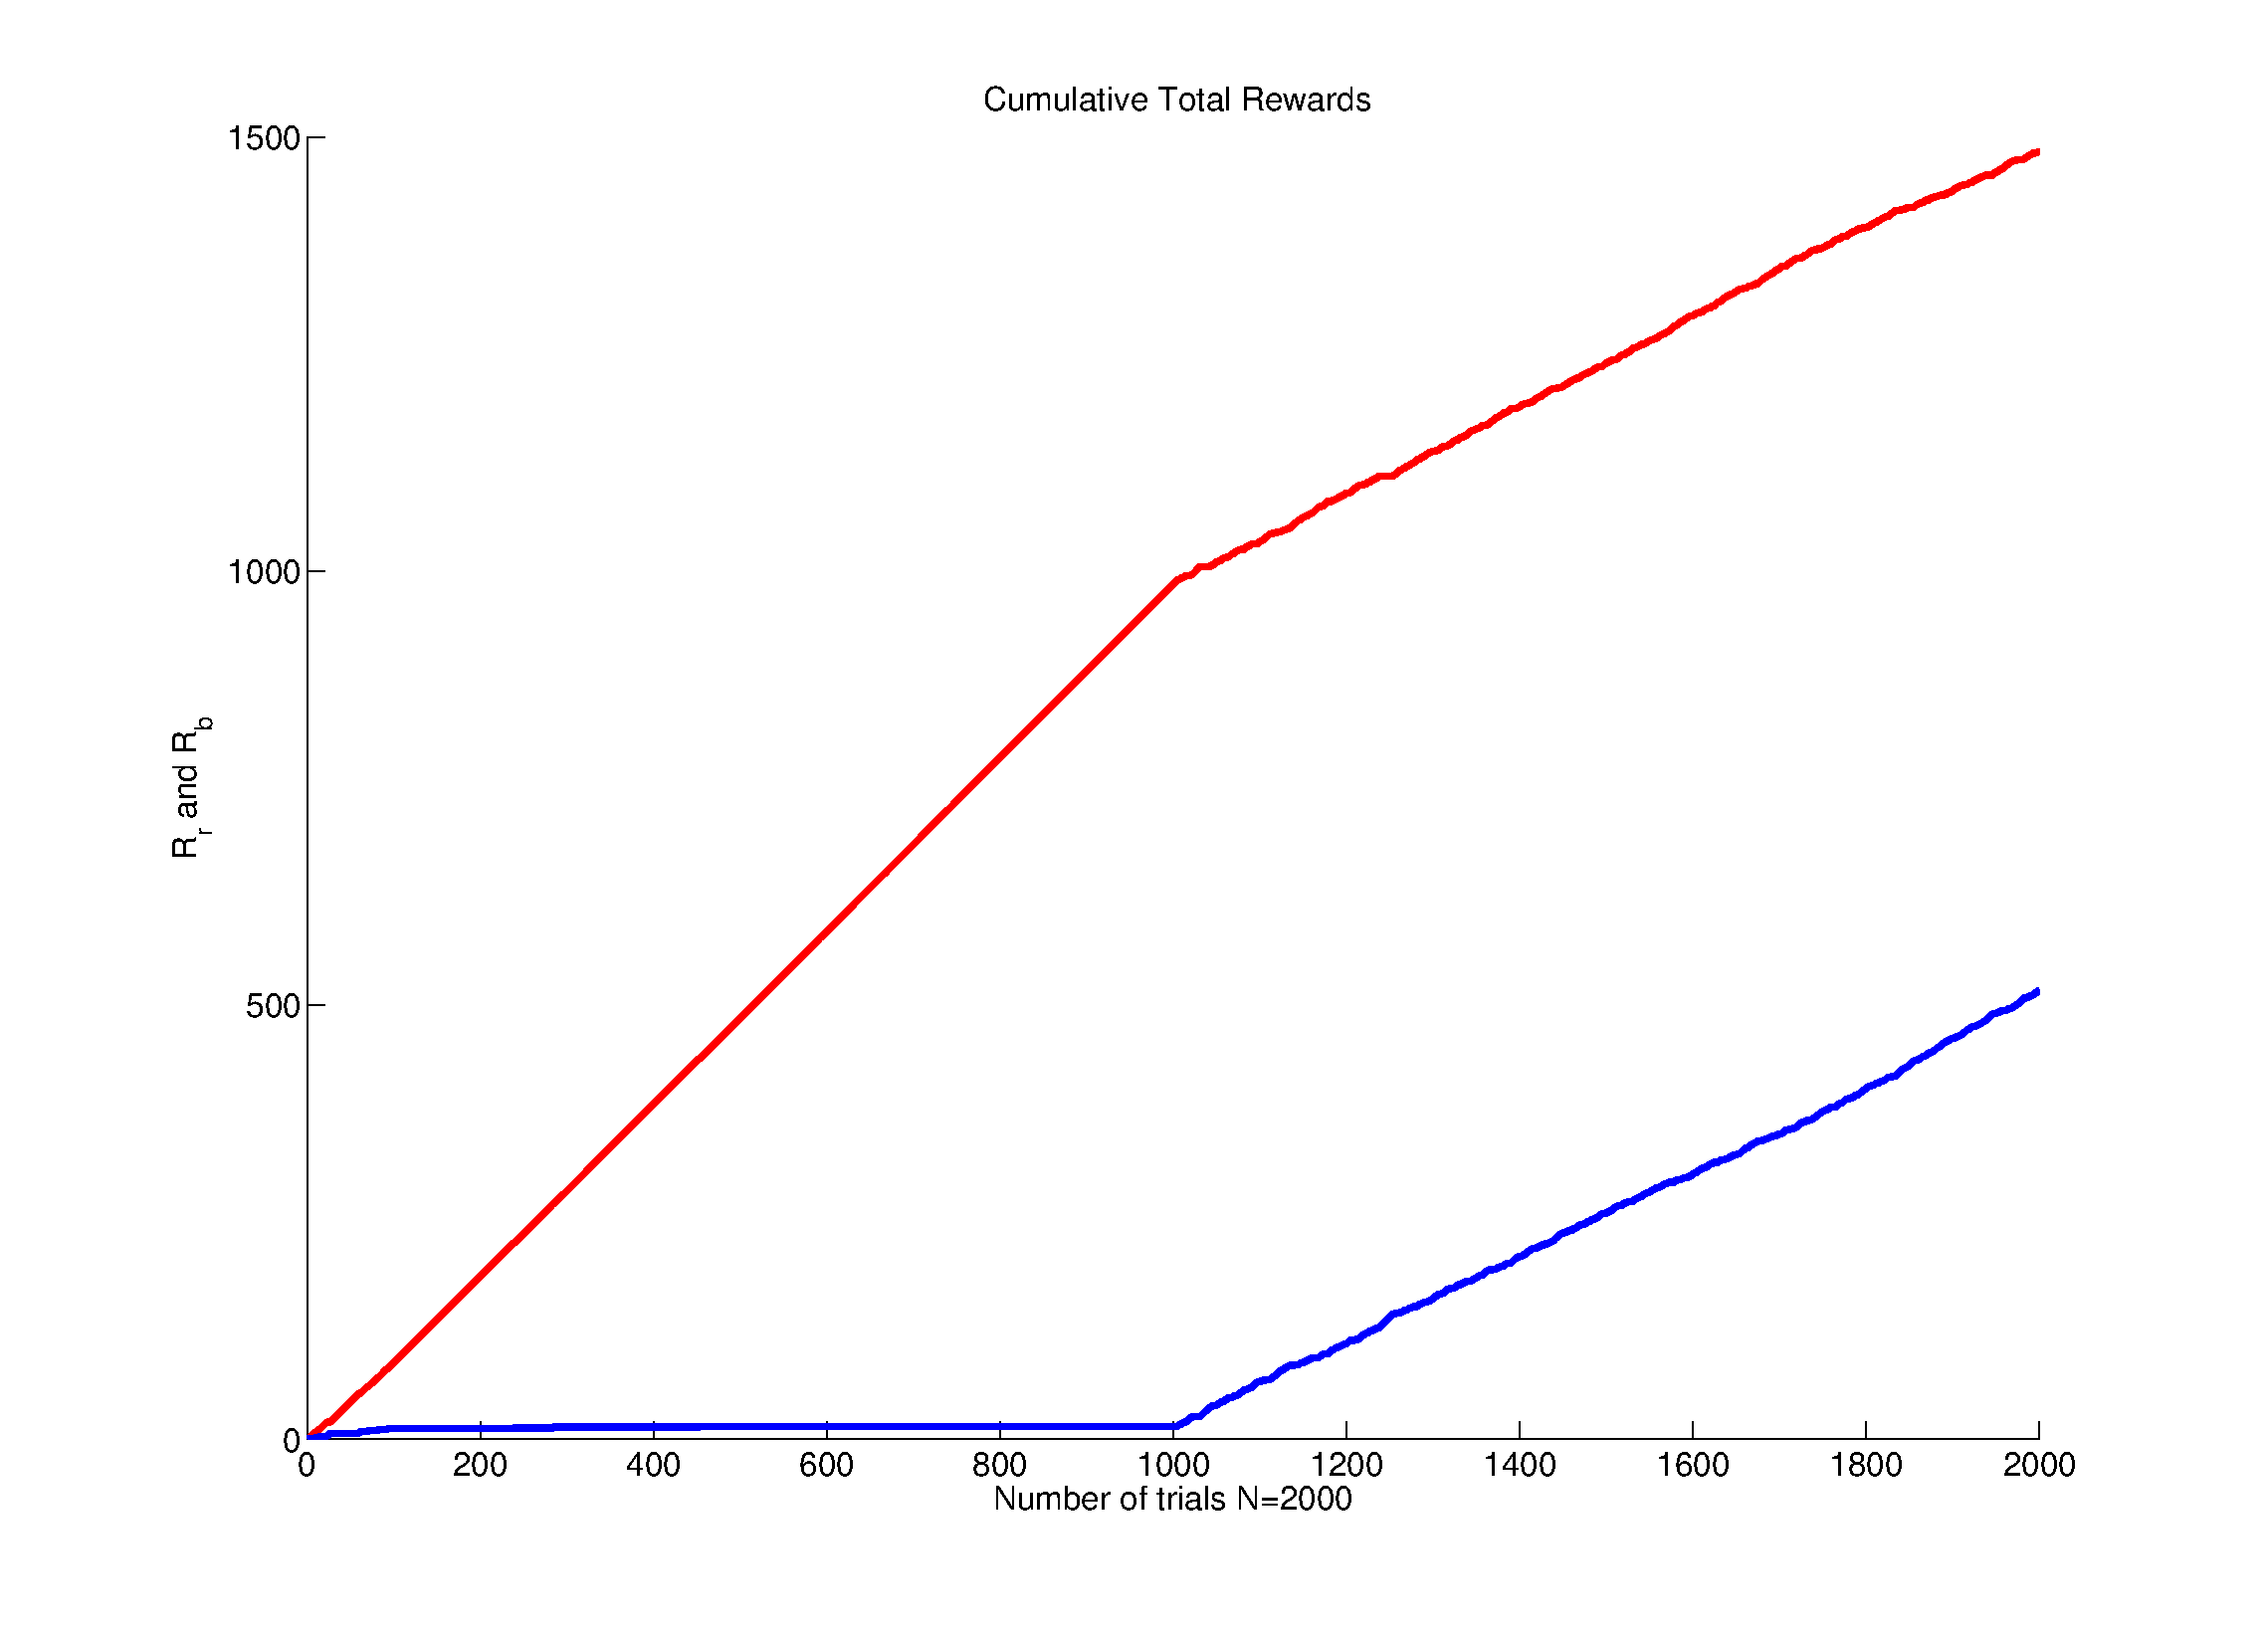
\includegraphics[width=\textwidth]{d_rew1.eps}
% tau4_M1.eps: 0x0 pixel, 300dpi, 0.00x0.00 cm, bb= -304   -42   918   834
\begin{footnotesize}
 Figure 15, $\beta=2$, $\epsilon=0.1$
\end{footnotesize}
\end{center}

\newpage
\begin{itemize}
 \item \textbf{ $\beta=20$, $\epsilon=0.1$}
\end{itemize}

\begin{center}
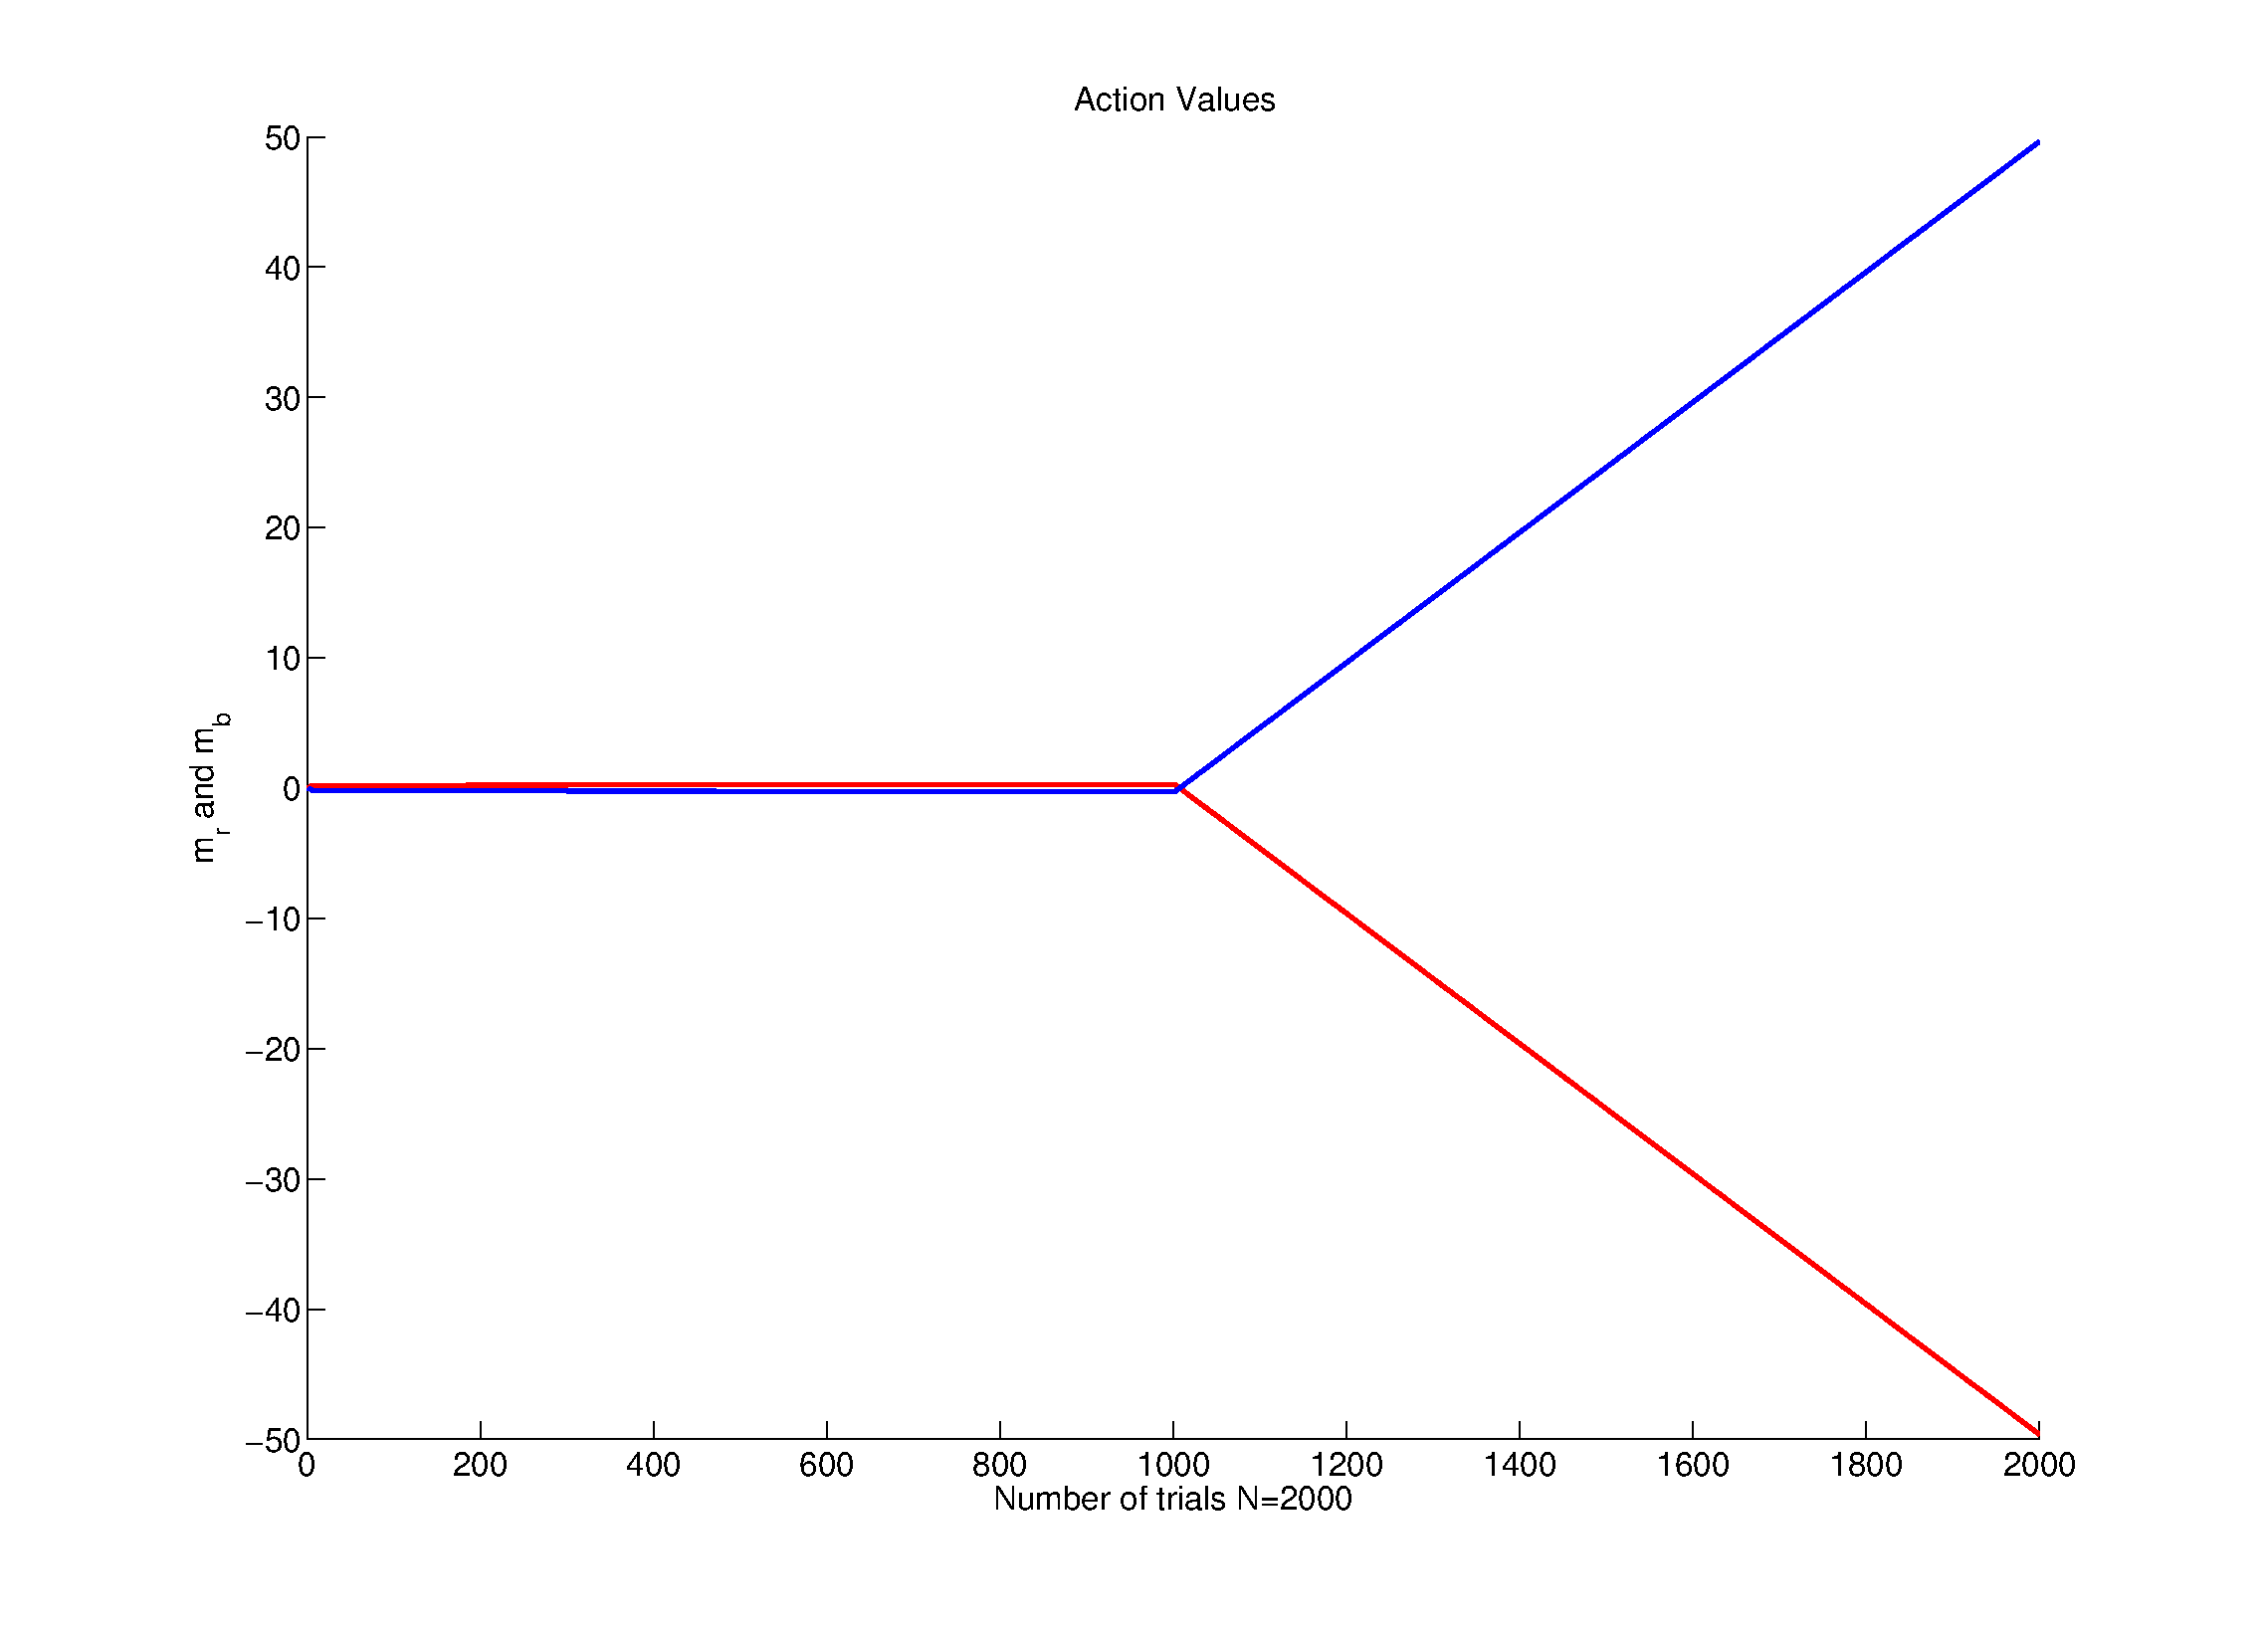
\includegraphics[width=\textwidth]{d_action2.eps}
% tau4_M1.eps: 0x0 pixel, 300dpi, 0.00x0.00 cm, bb= -304   -42   918   834
\begin{footnotesize}
 Figure 16, $\beta=20$, $\epsilon=0.1$
\end{footnotesize}
\end{center}

\begin{center}
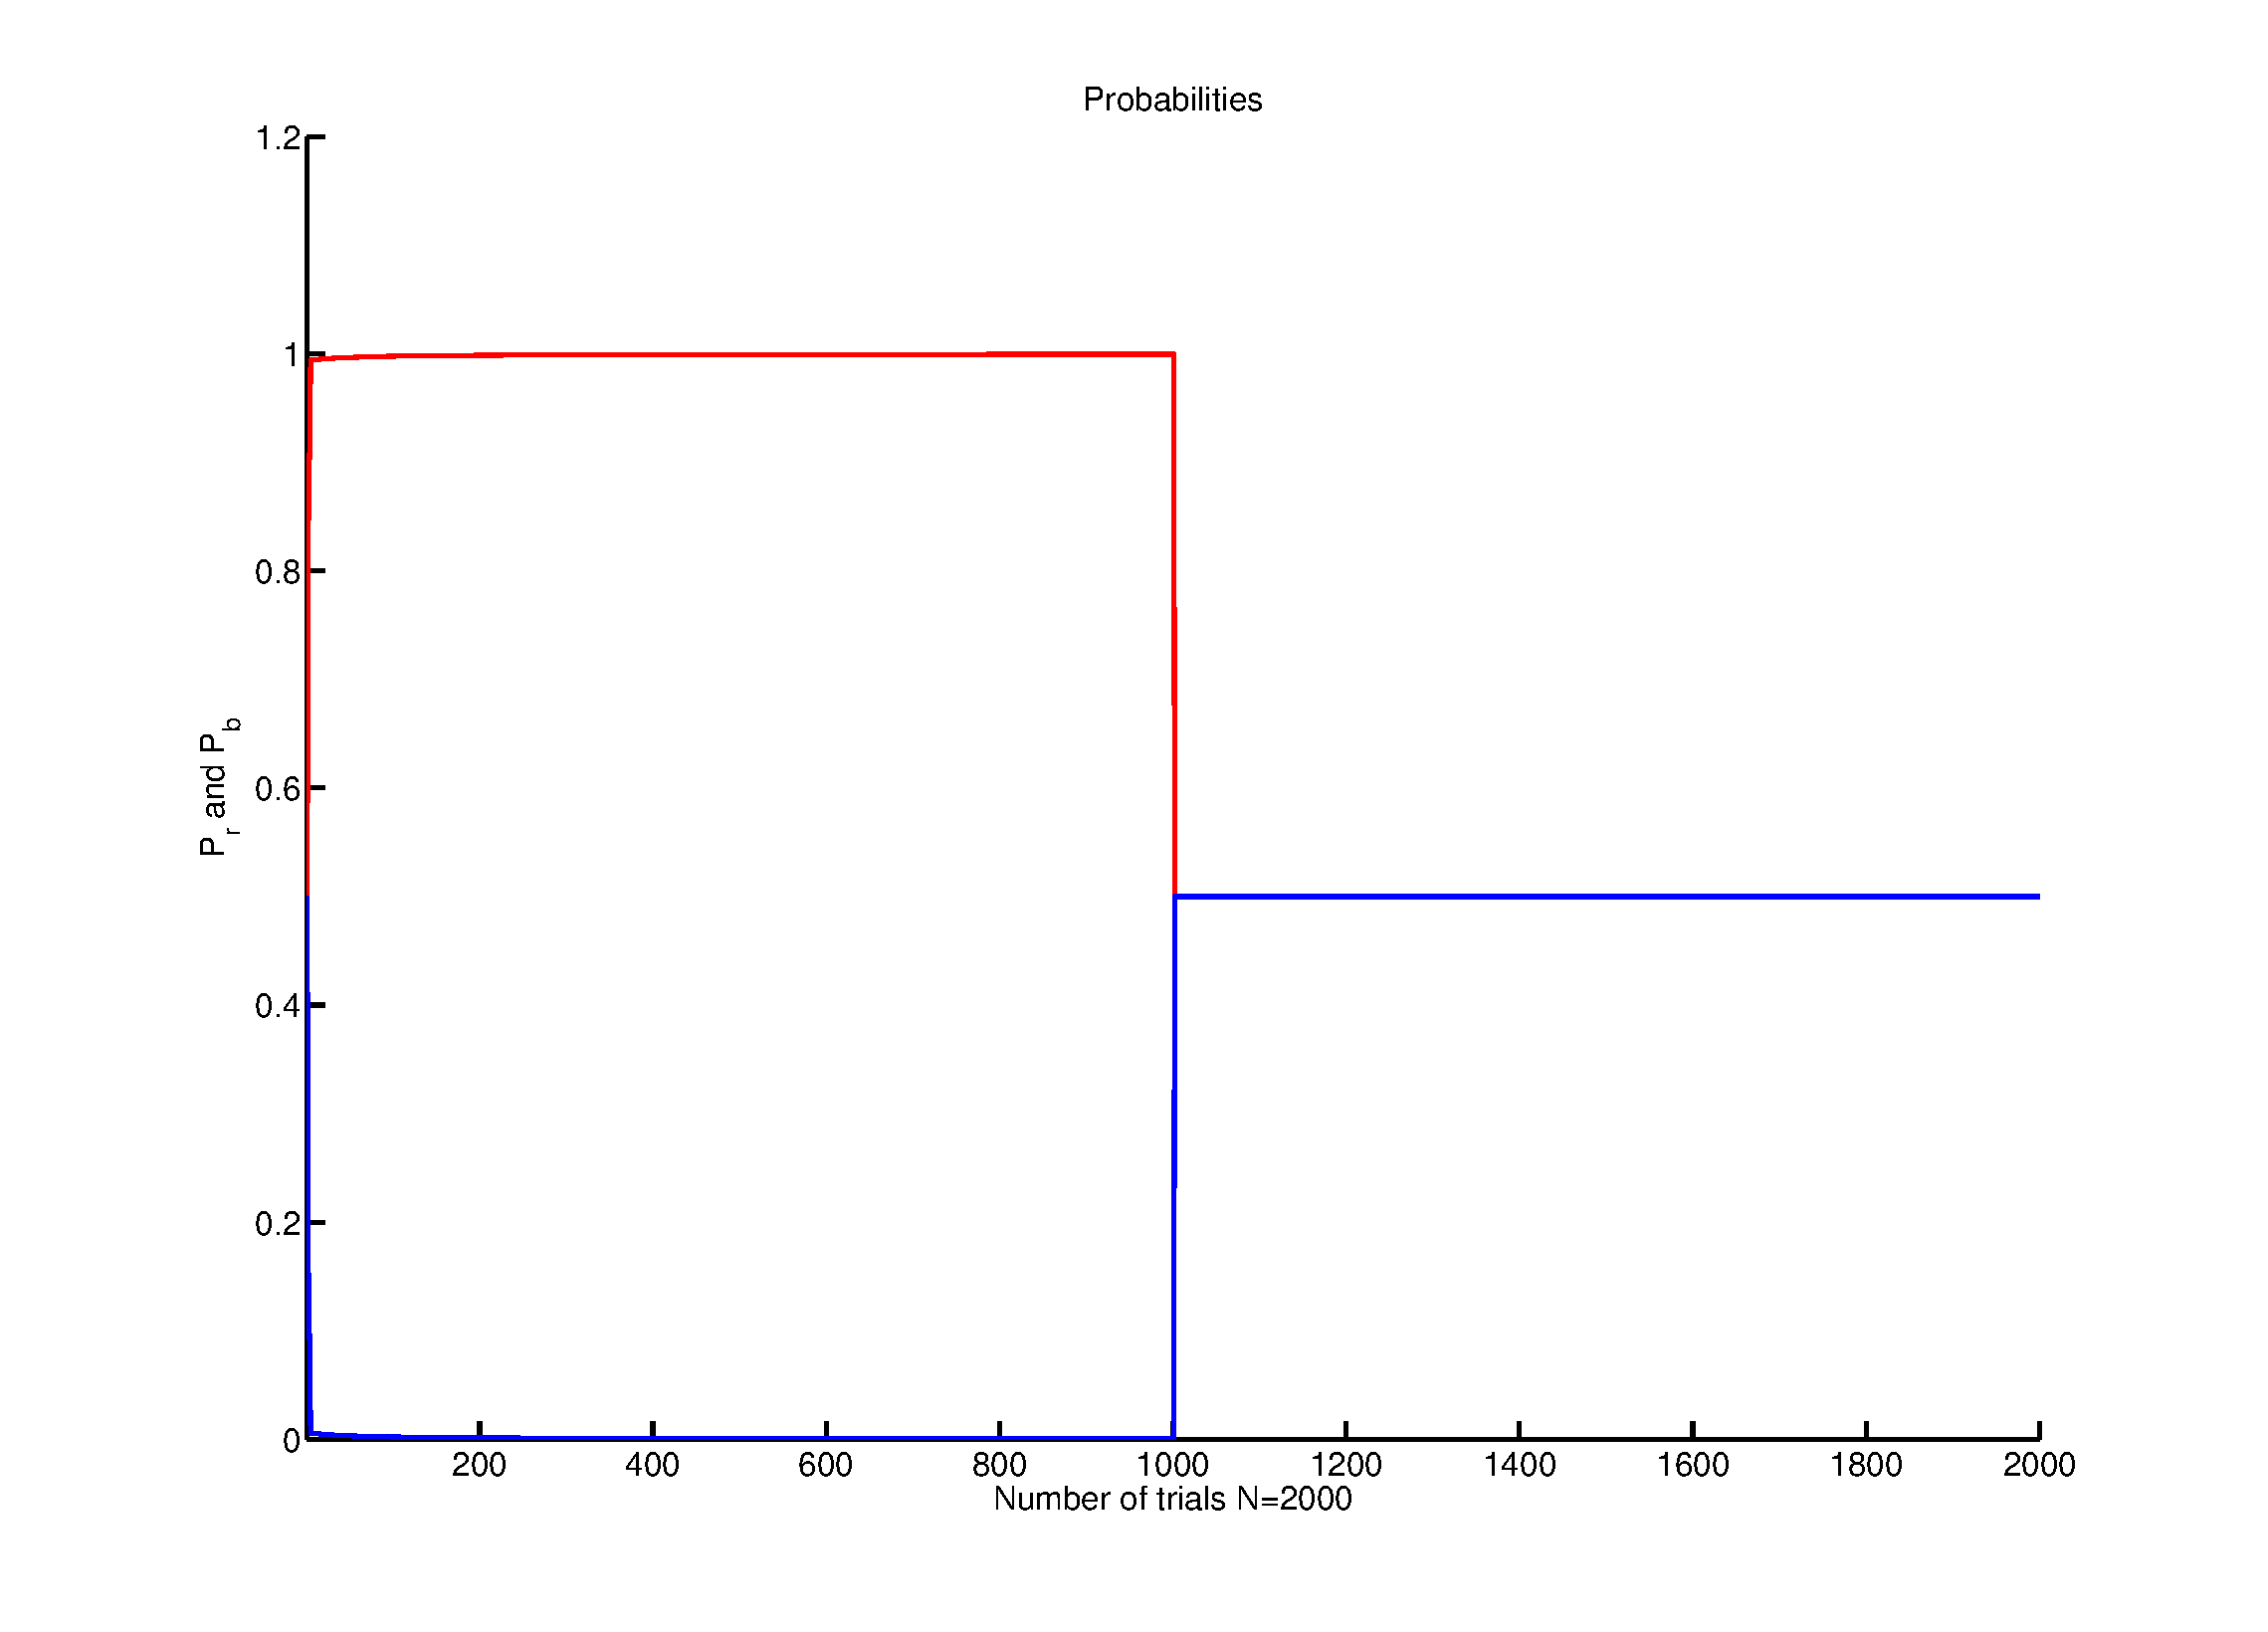
\includegraphics[width=\textwidth]{d_prob2.eps}
% tau4_M1.eps: 0x0 pixel, 300dpi, 0.00x0.00 cm, bb= -304   -42   918   834
\begin{footnotesize}
 Figure 17, $\beta=20$, $\epsilon=0.1$
\end{footnotesize}
\end{center}

\begin{center}
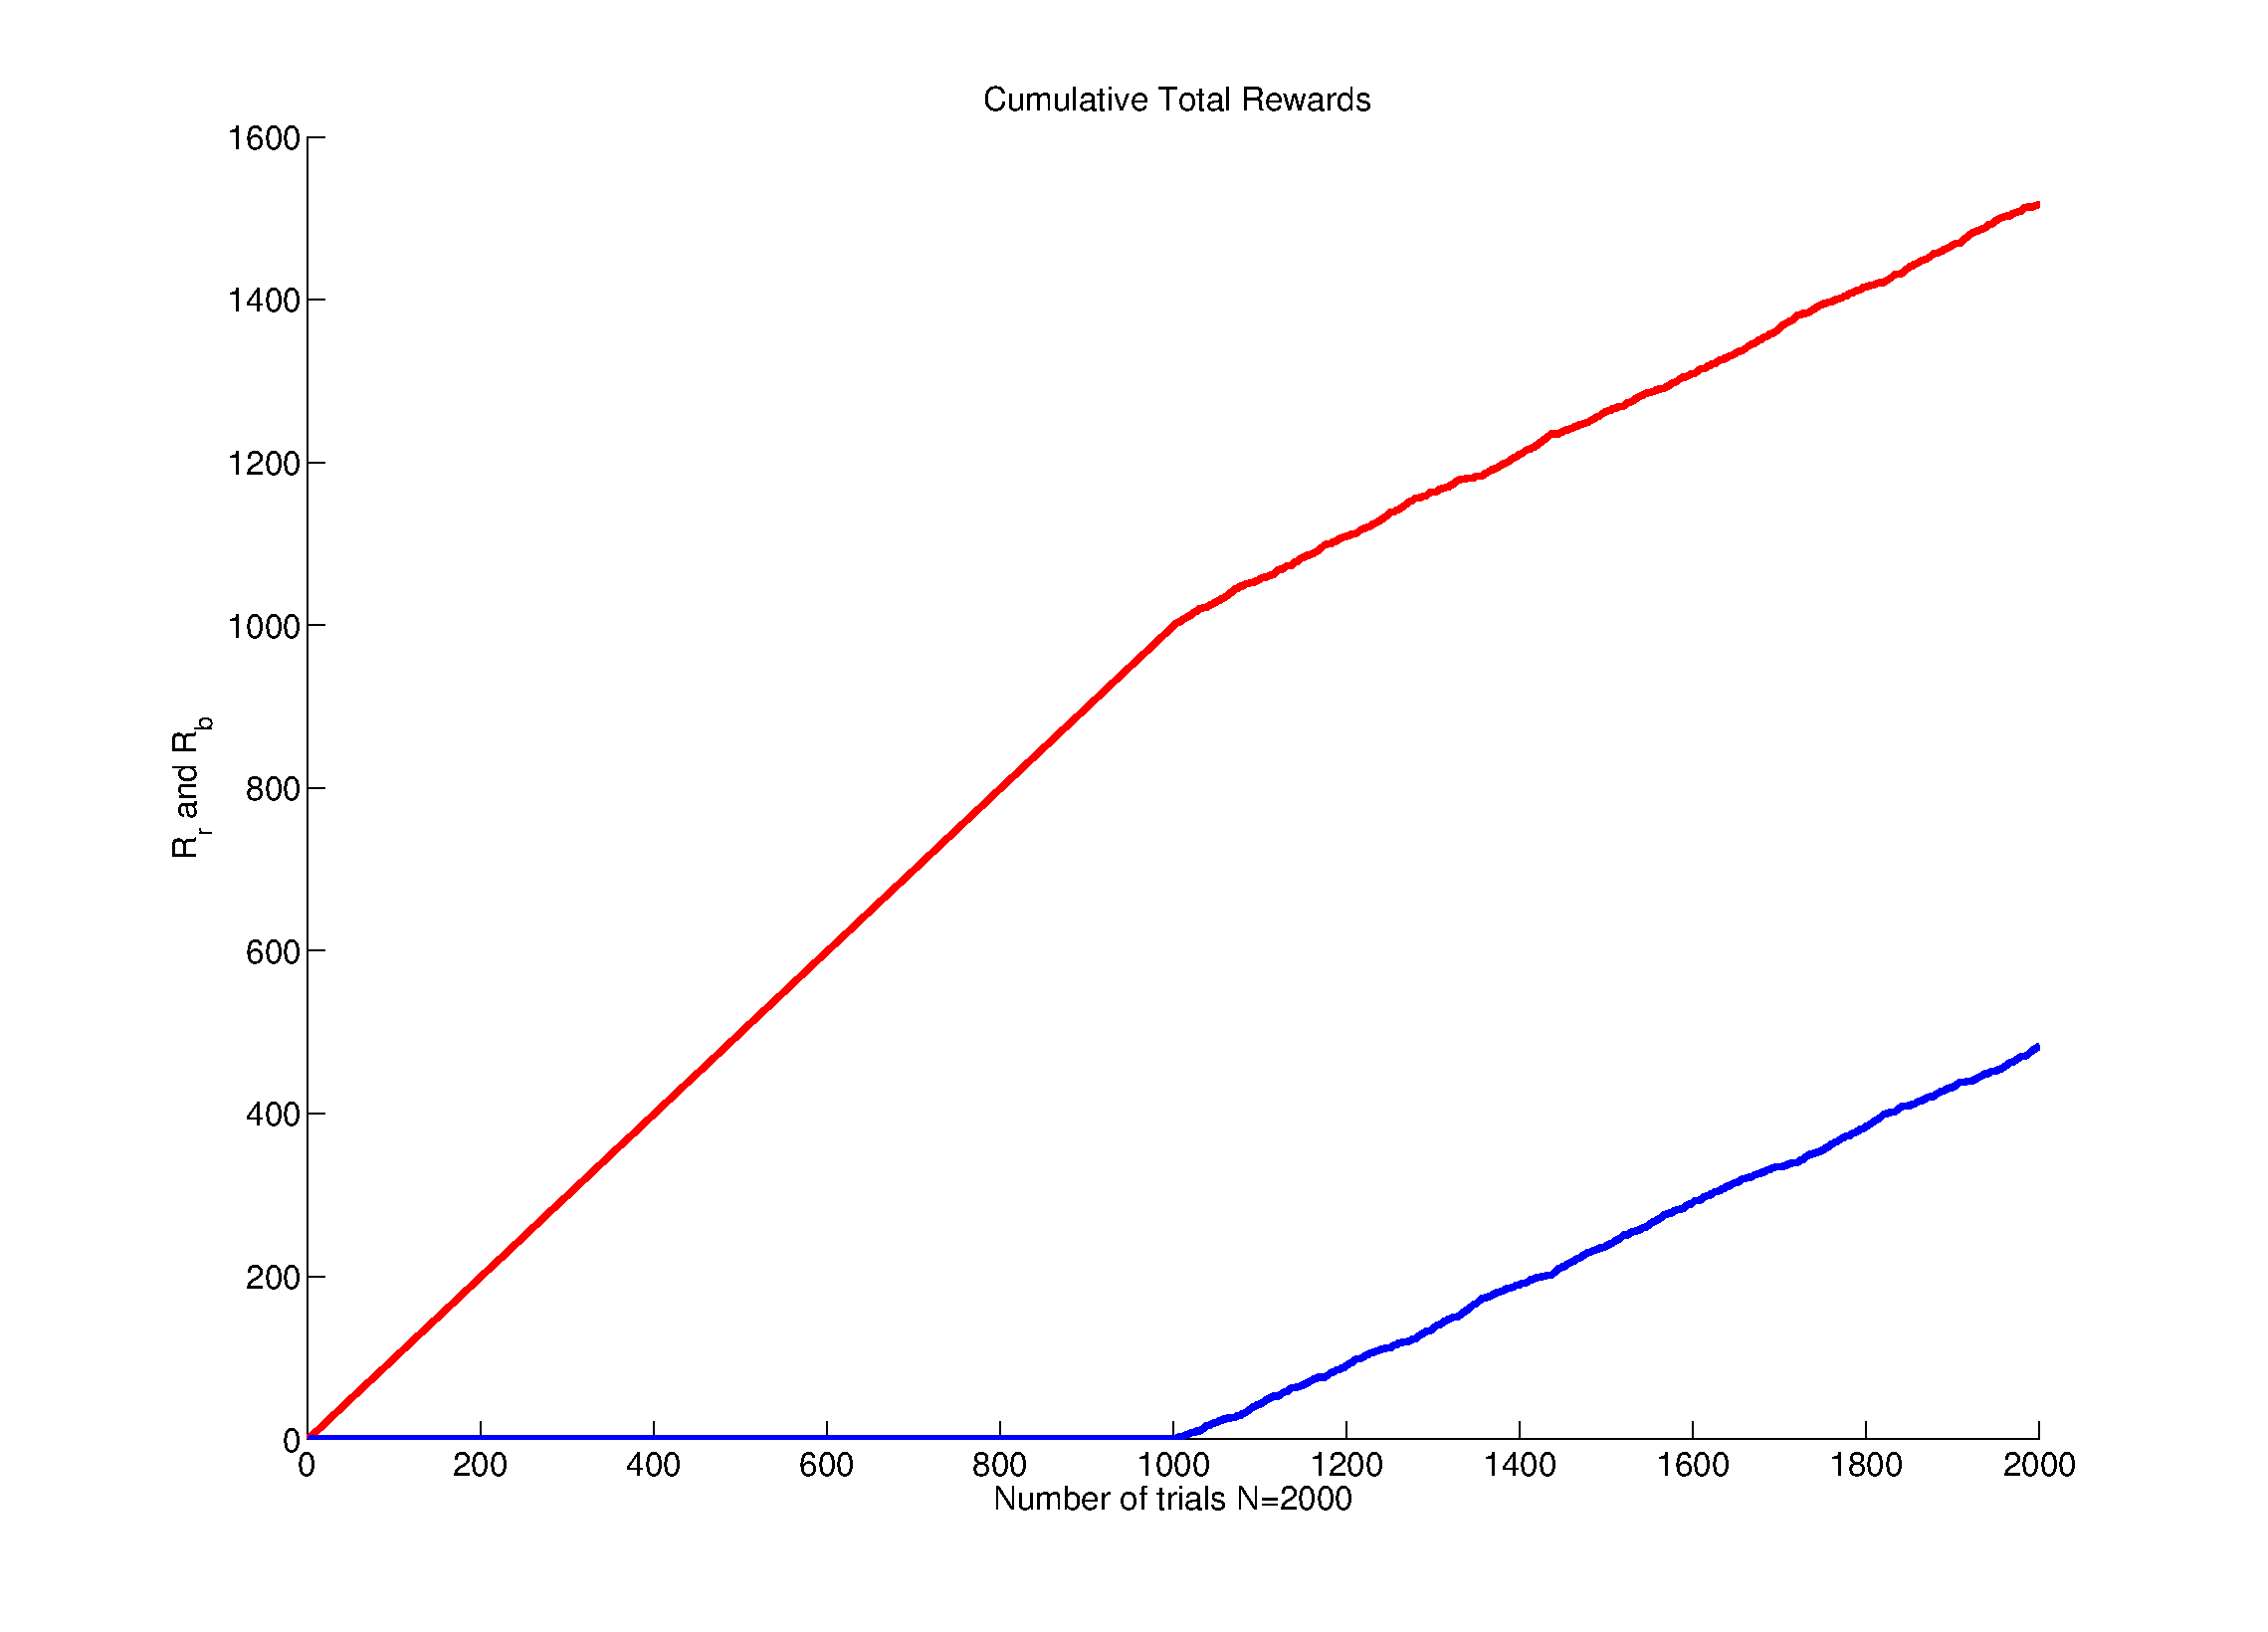
\includegraphics[width=\textwidth]{d_rew2.eps}
% tau4_M1.eps: 0x0 pixel, 300dpi, 0.00x0.00 cm, bb= -304   -42   918   834
\begin{footnotesize}
 Figure 18, $\beta=20$, $\epsilon=0.1$
\end{footnotesize}
\end{center}

\begin{itemize}
 \item \textbf{ $\beta=2$, $\epsilon=0.01$}
\end{itemize}

\begin{center}
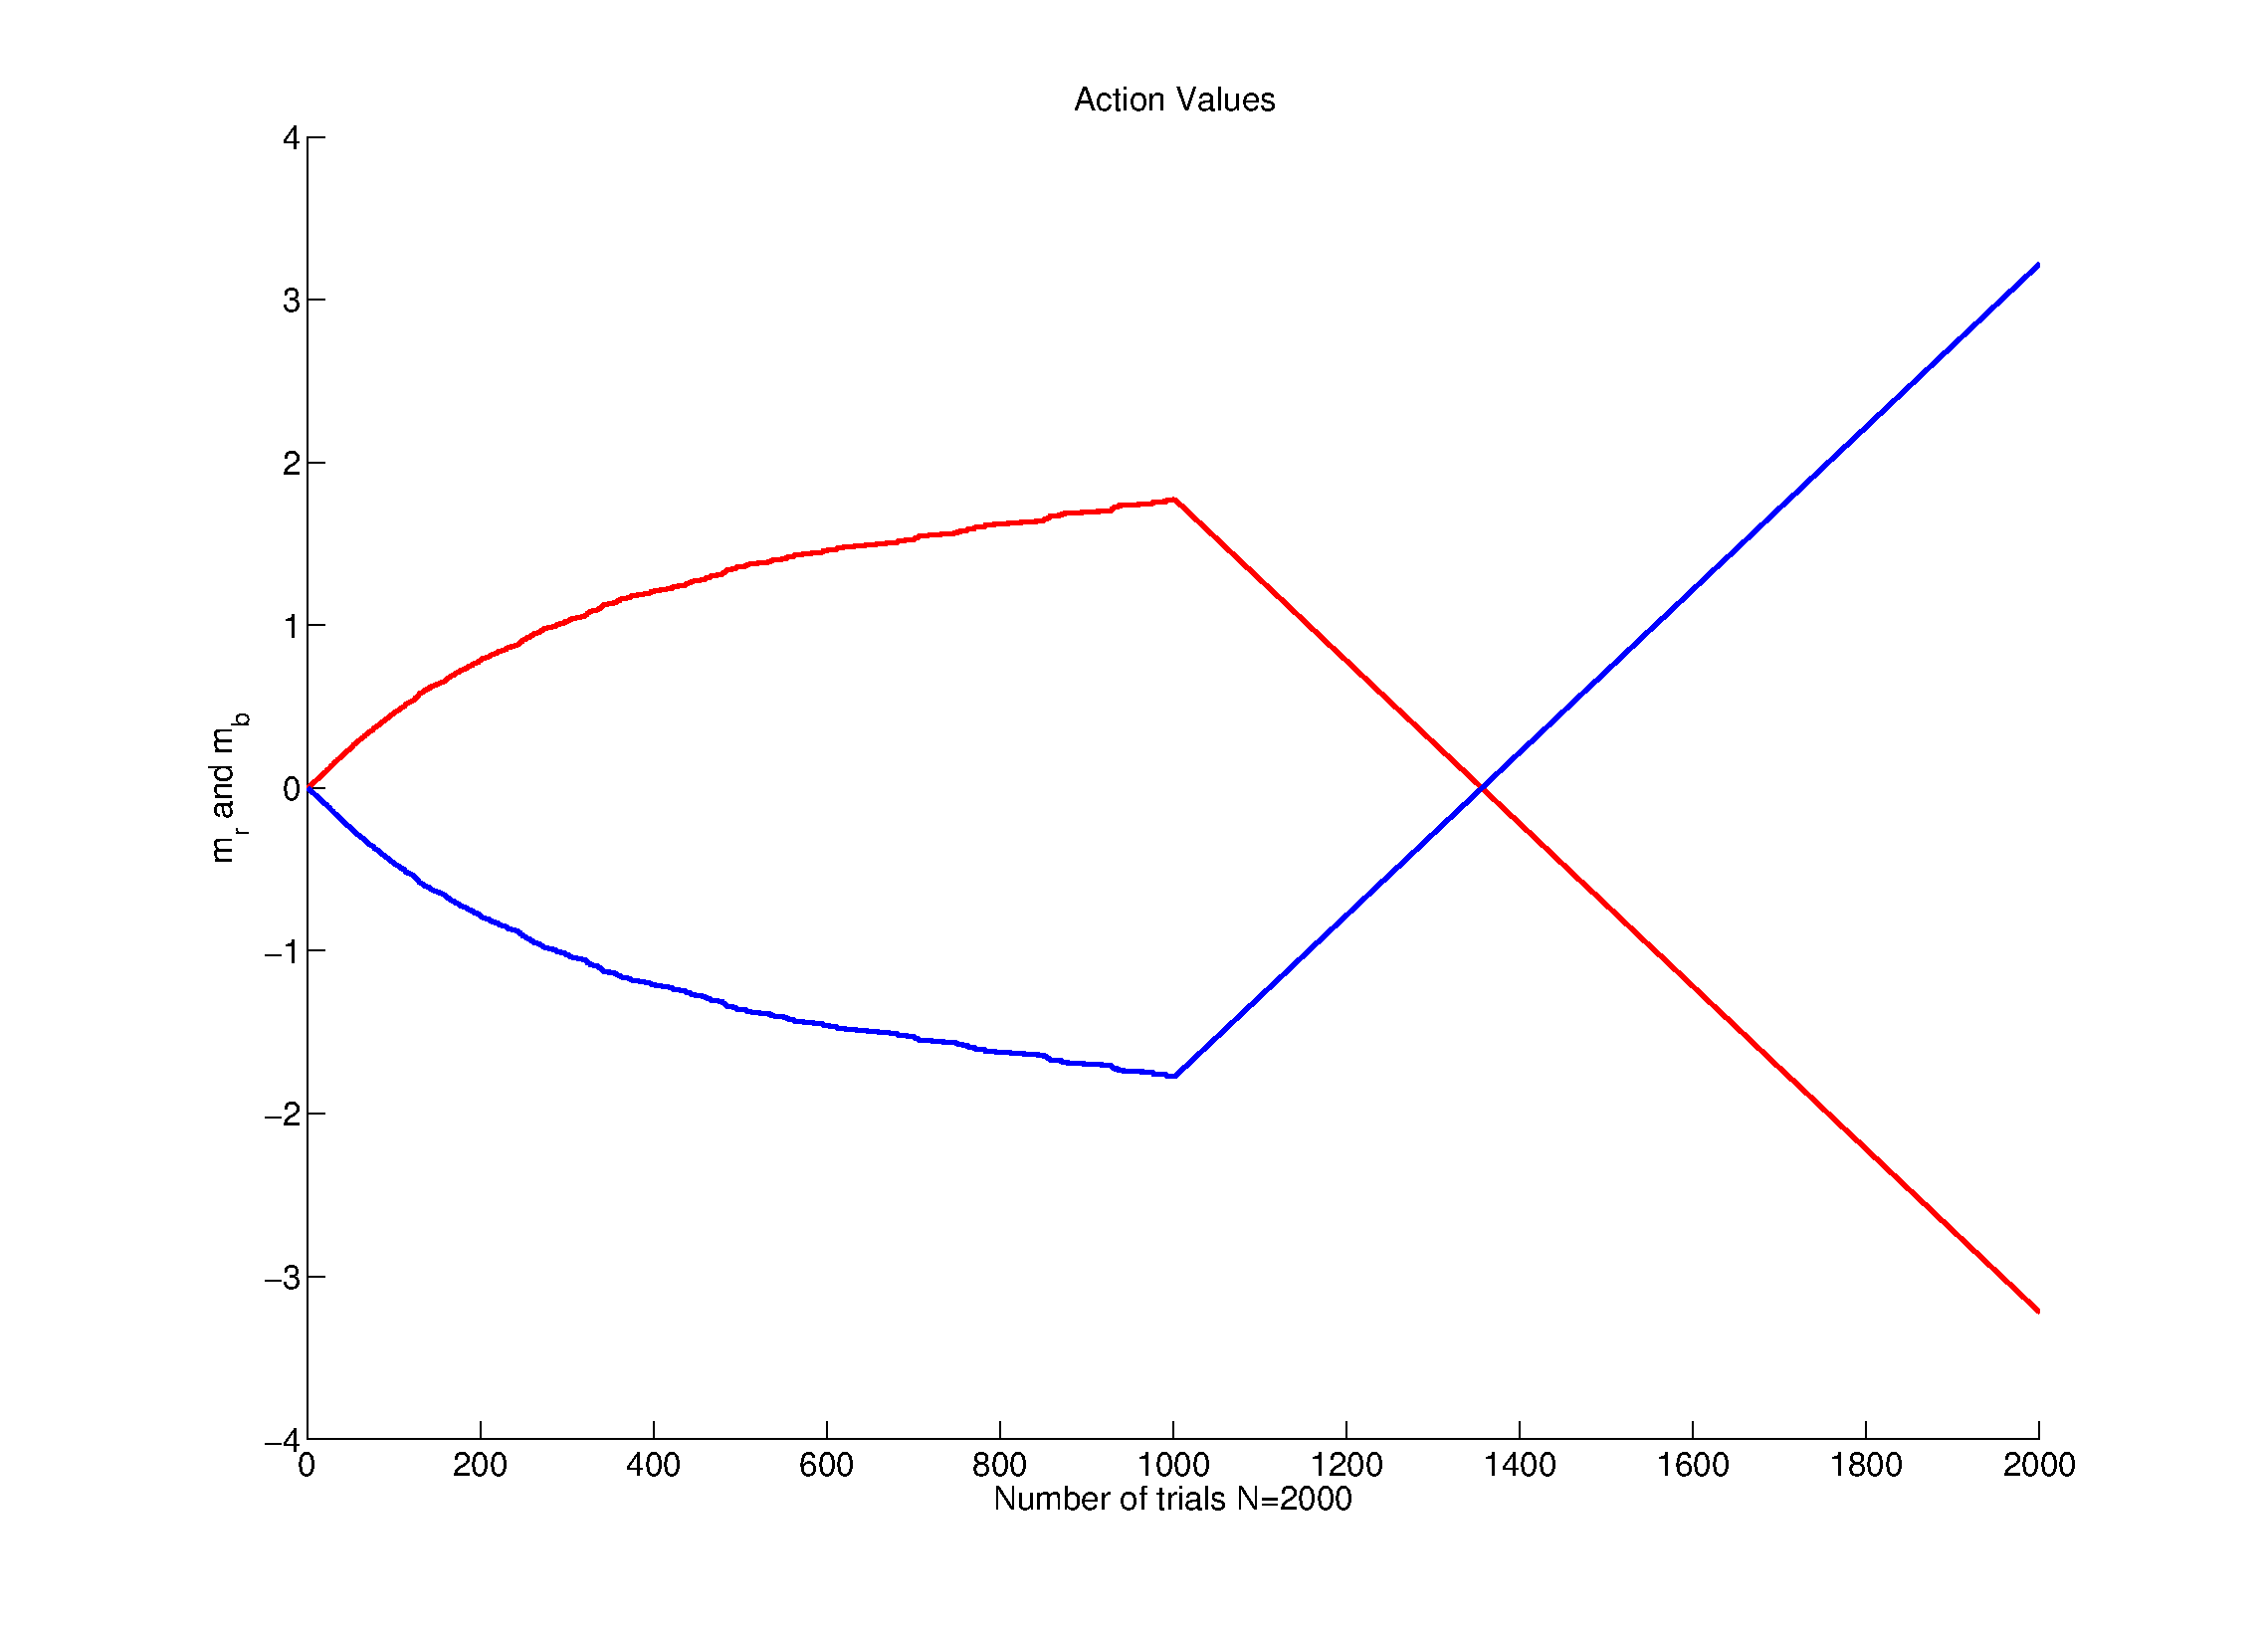
\includegraphics[width=\textwidth]{d_action3.eps}
% tau4_M1.eps: 0x0 pixel, 300dpi, 0.00x0.00 cm, bb= -304   -42   918   834
\begin{footnotesize}
 Figure 19, $\beta=2$, $\epsilon=0.01$
\end{footnotesize}
\end{center}

\begin{center}
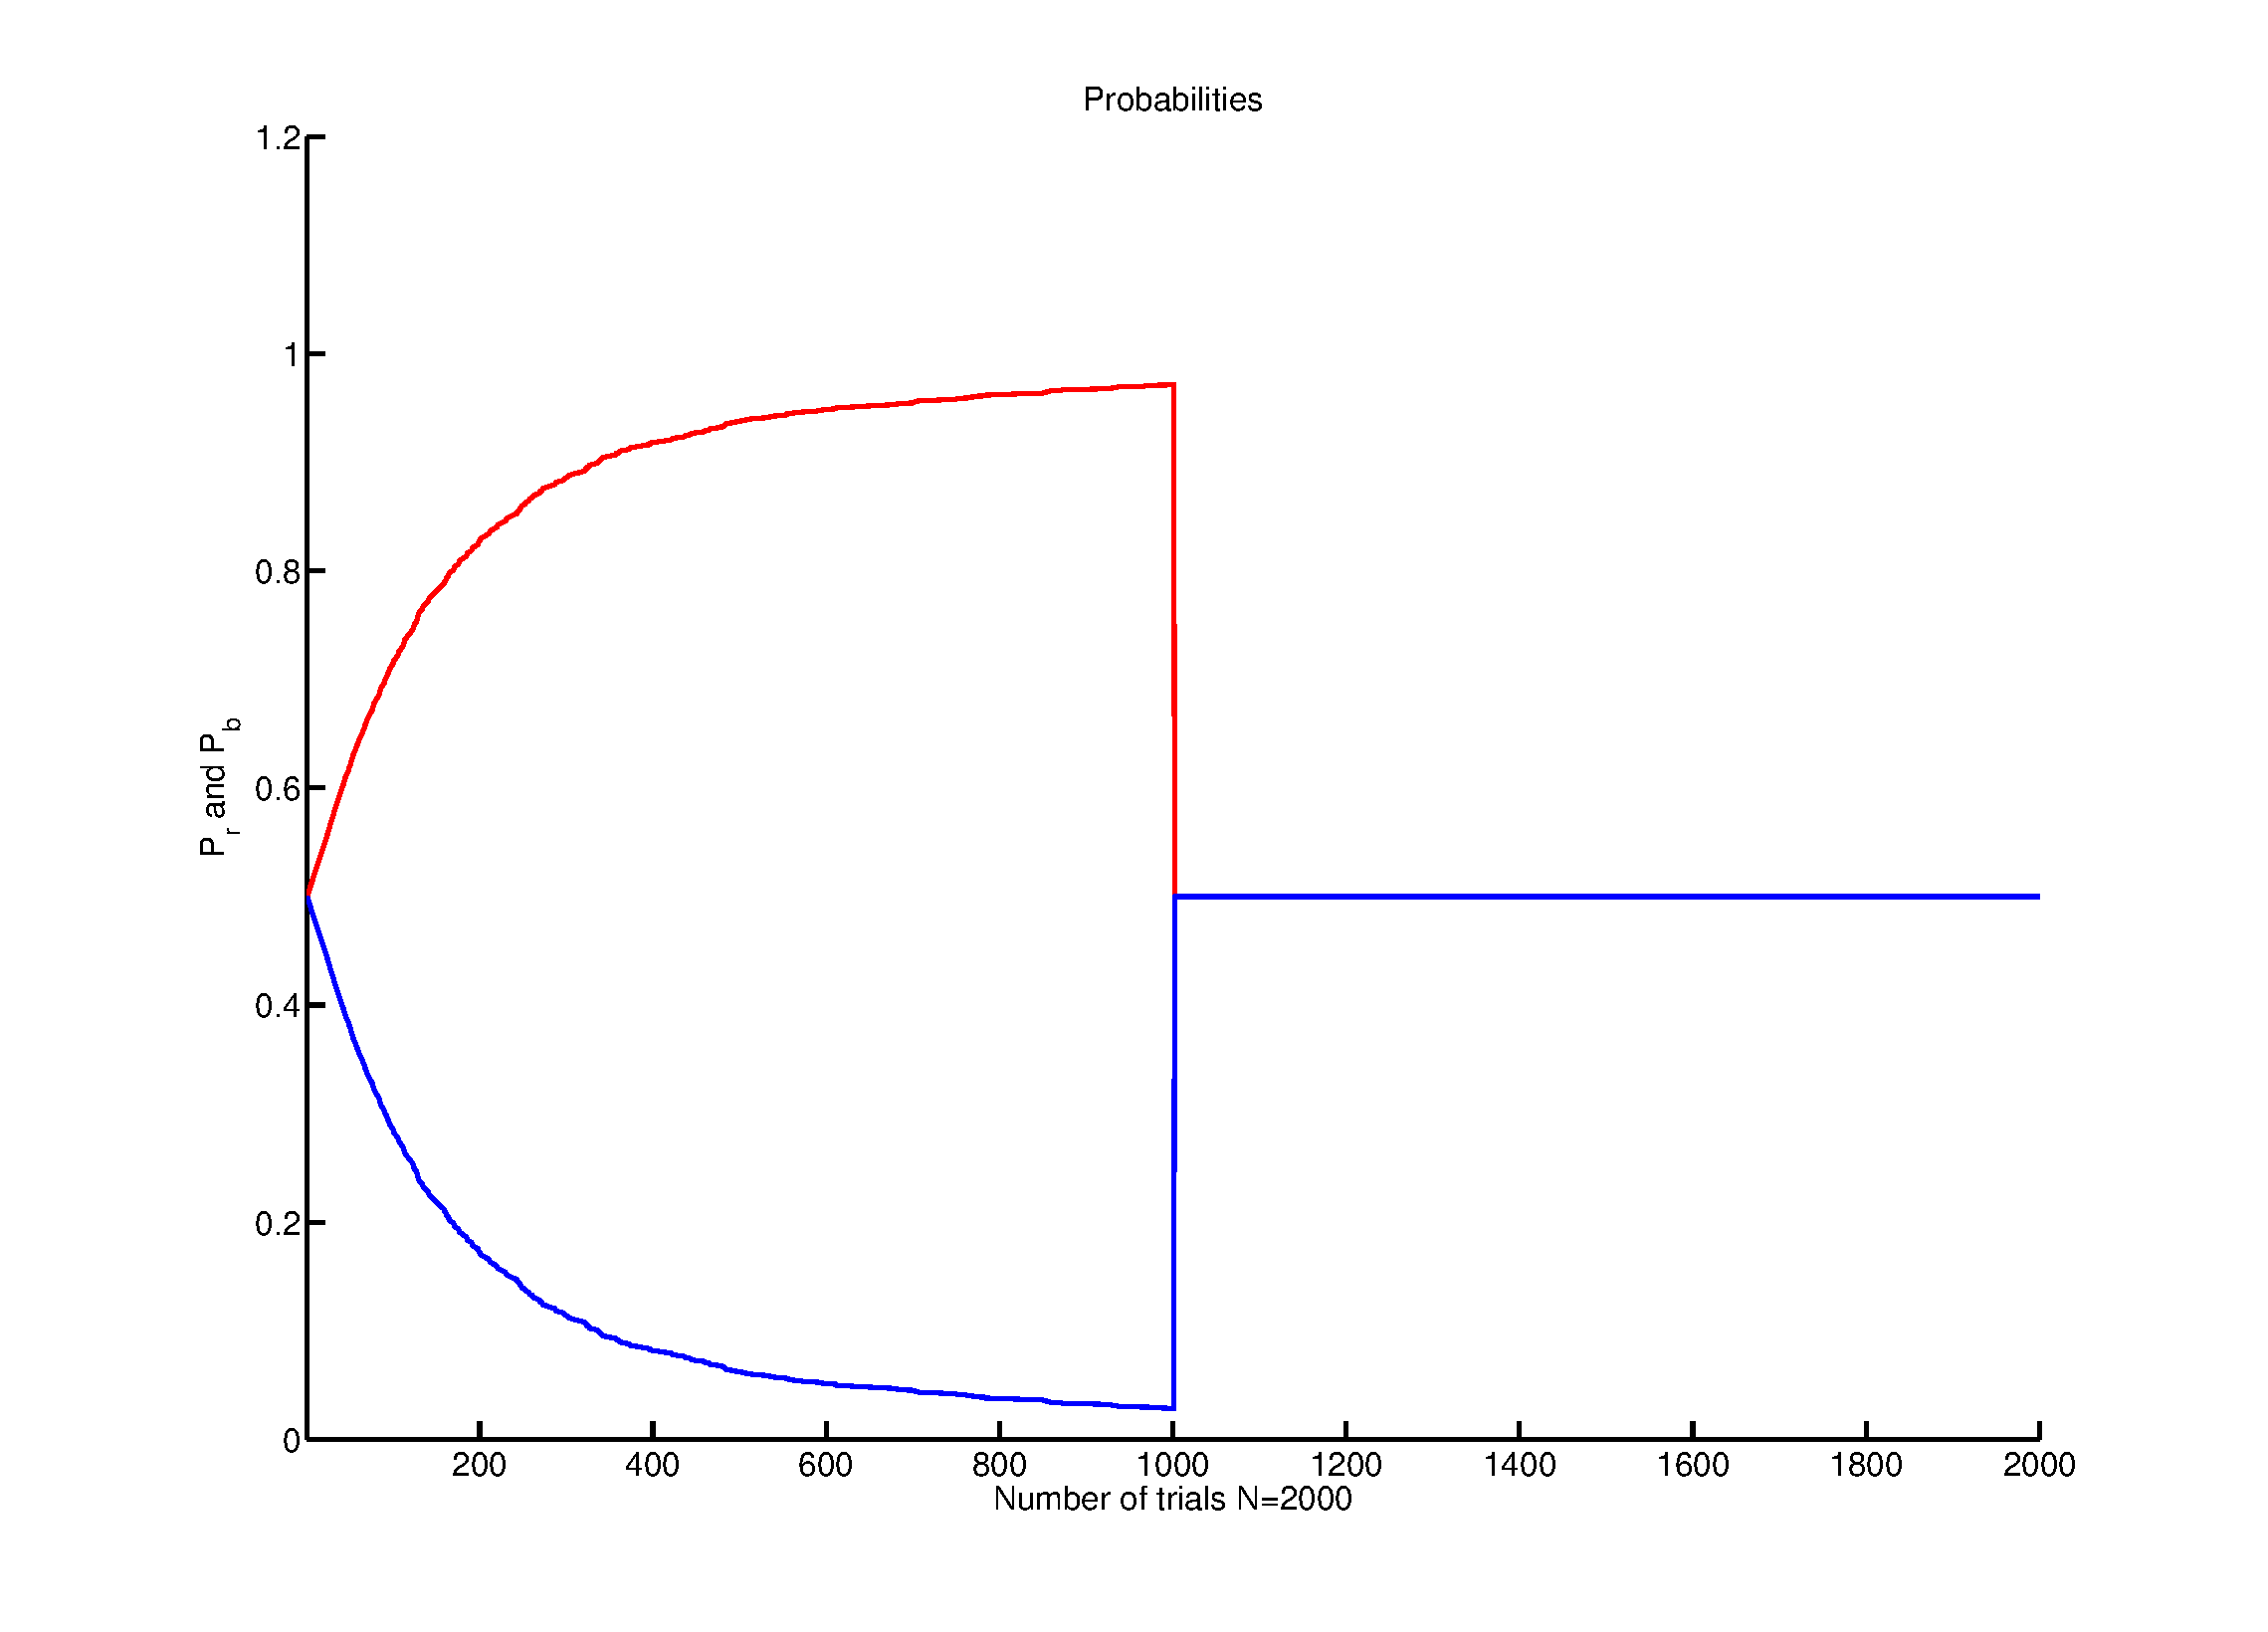
\includegraphics[width=\textwidth]{d_prob3.eps}
% tau4_M1.eps: 0x0 pixel, 300dpi, 0.00x0.00 cm, bb= -304   -42   918   834
\begin{footnotesize}
 Figure 20, $\beta=2$, $\epsilon=0.01$
\end{footnotesize}
\end{center}

\begin{center}
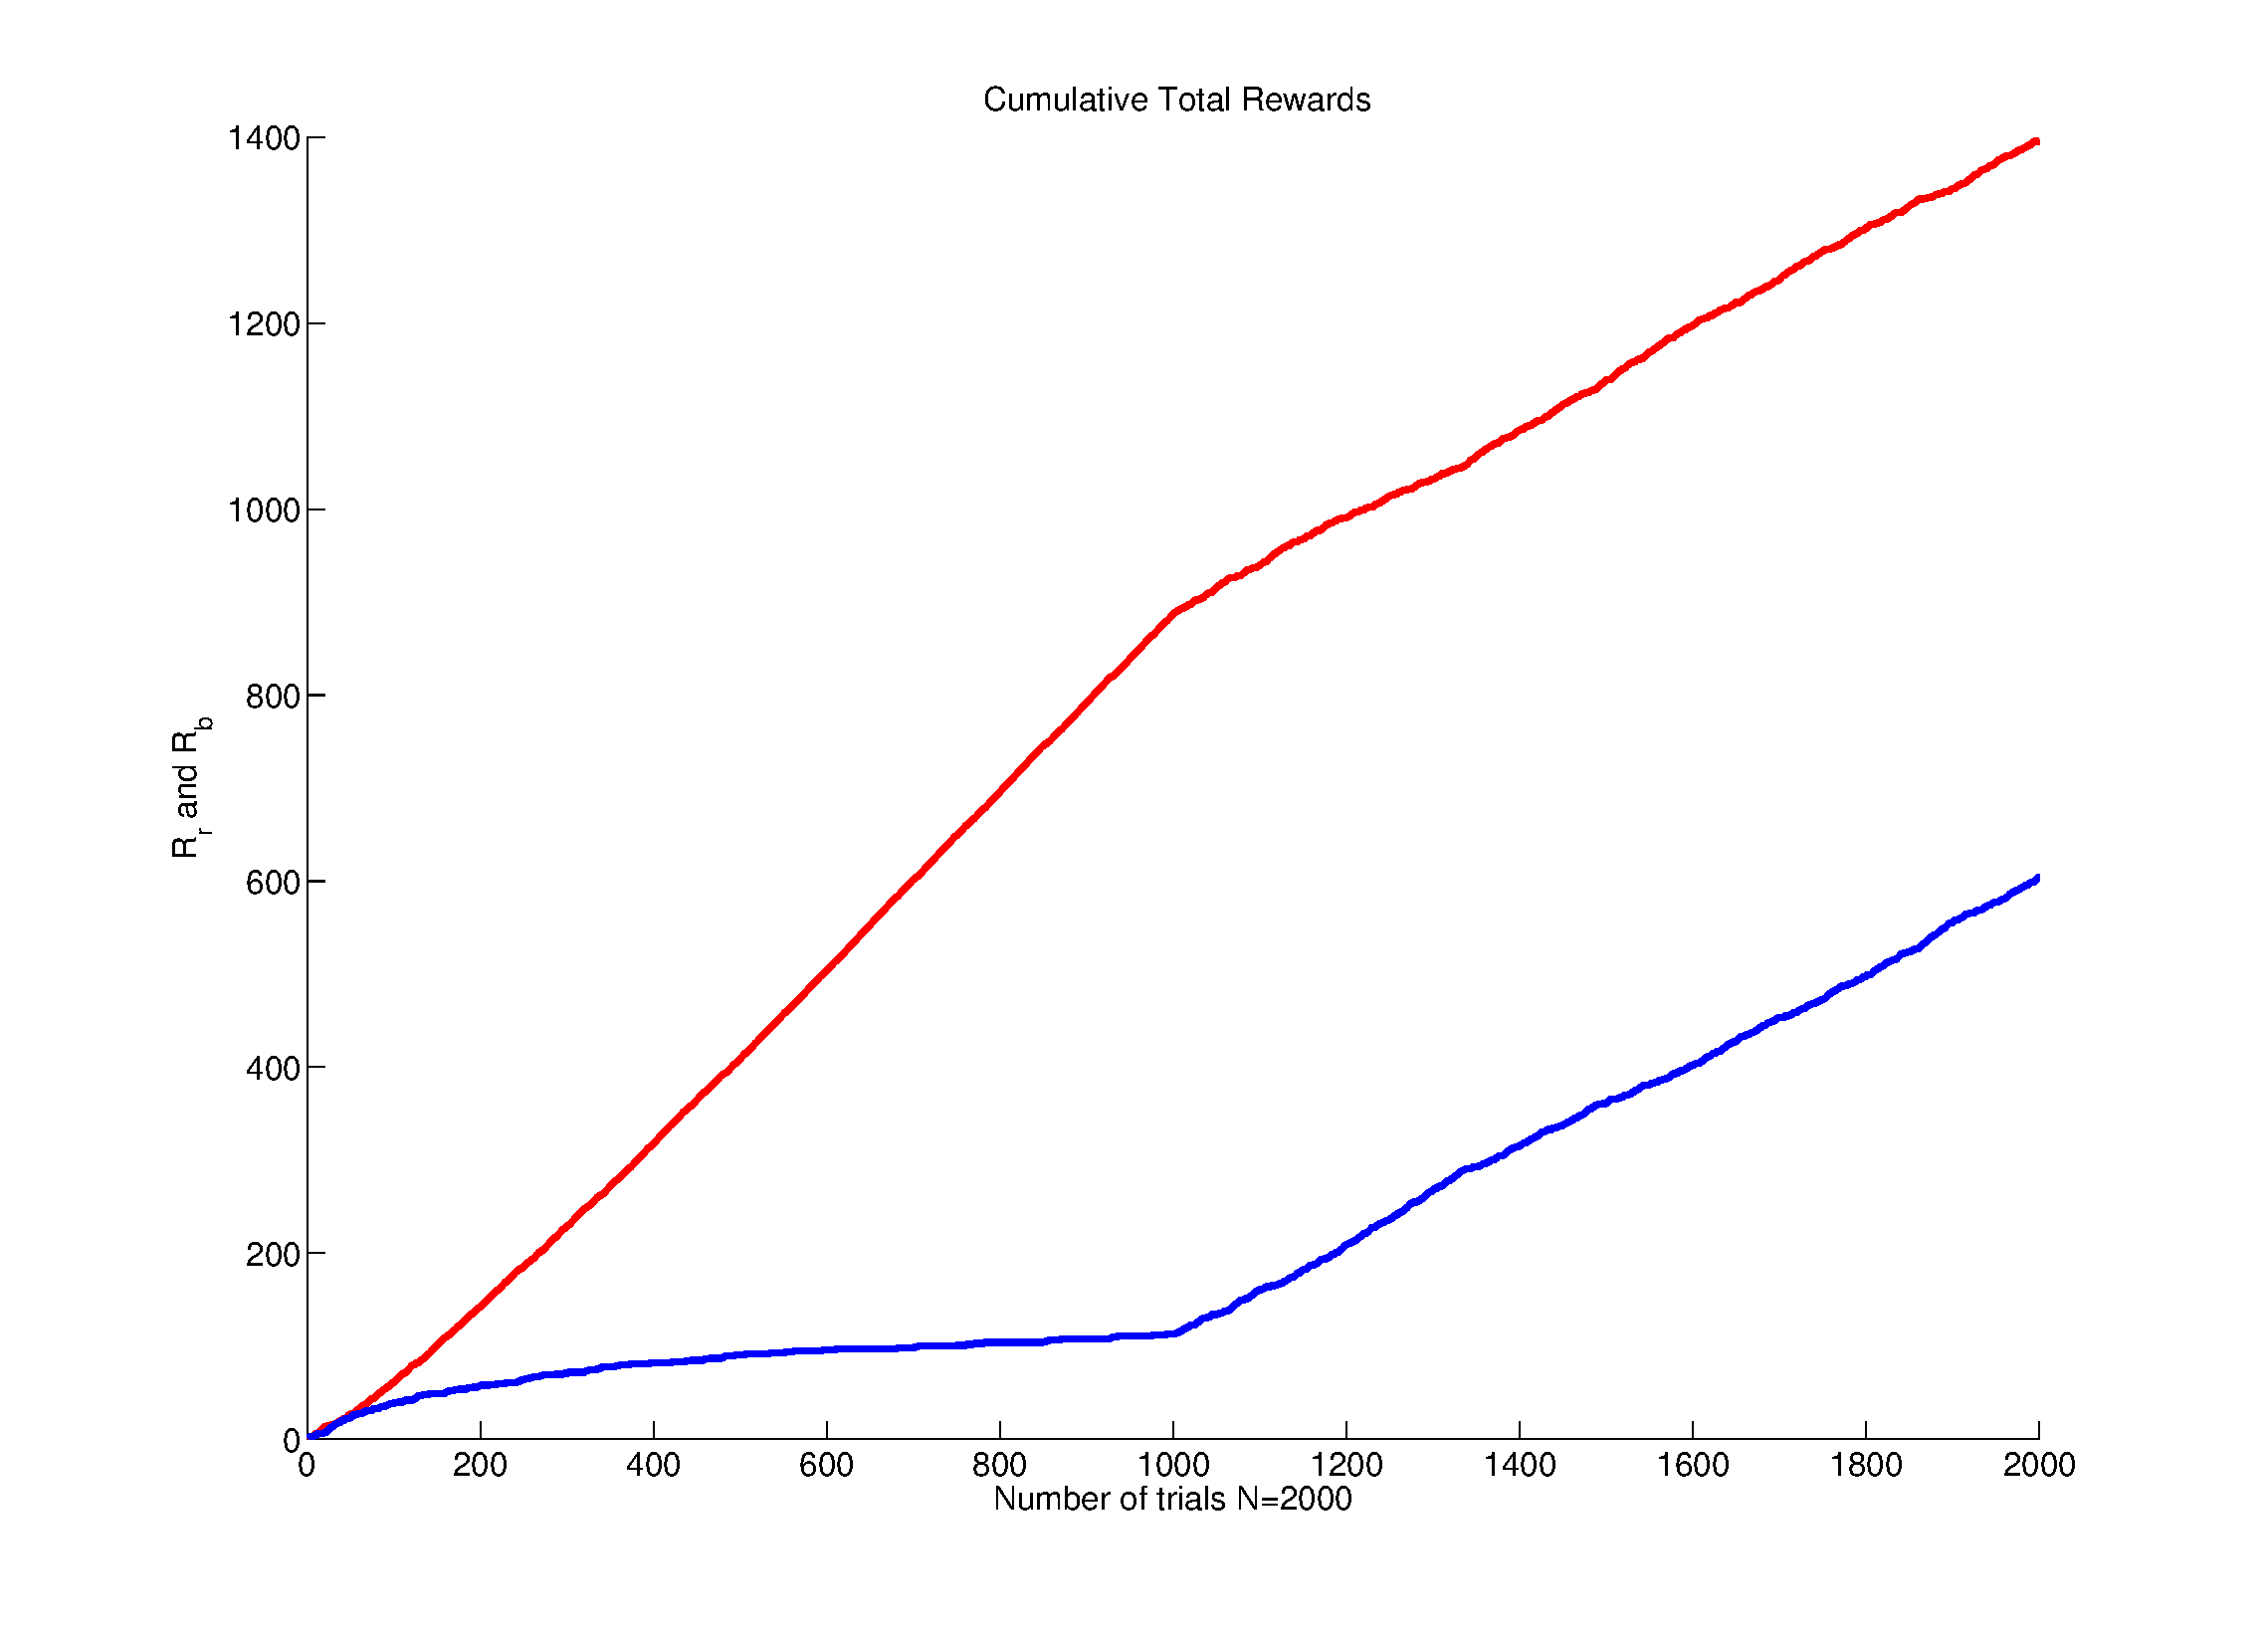
\includegraphics[width=\textwidth]{d_rew3.eps}
% tau4_M1.eps: 0x0 pixel, 300dpi, 0.00x0.00 cm, bb= -304   -42   918   834
\begin{footnotesize}
 Figure 21, $\beta=2$, $\epsilon=0.01$
\end{footnotesize}
\end{center}

\subsection{Discussion}
\begin{itemize}
 \item The $\beta$ value still determines the exploitation/exploration balance. When $\beta$ increases, learning capacity of bee performes well.
\item The action values in direct actor model are incremented for all actions, taken or not, and have arbitrary units. 
\item With a small $\epsilon$ value, the action values seem to be more separated at the first phase, Figure 19, in comparison to Figure 10. This reflects on the probabilities such that, the probability to choose the blue flower in first phase does not drop immediately to 0, instead it converges to zero exponentially, Figure 20. Additionally, the smaller the $\epsilon$ is, the poorer to learning performance is, Figure 21.
\item In all casesm the action values converge at one point to the average action value ${\bar m}$. The duration how long it takes to converge to ${\bar m}$ is decided by $\beta$ and $\epsilon$ values. For instance, for a smaller $\epsilon=0.01$ value, it takes more trials to converge $m_r$ and $m_b$ to ${\bar m}$, Figure 19, in comparison to Figure 13 ($\epsilon=0.1$). Additionally, $\epsilon$ seems to affect the incline of sigmoidal probability functions e.g Figure 14 and Figure 20.
\item Indirect model brings us more complexity, but sometimes with more efficiency. The direct actor moder seems to be simpler, but with less efficieny. 
\end{itemize}



\end{document}
